\documentclass{tufte-handout}

\title{MATH 27300 Lecture Notes}

\author{Marcus Kuo}

\date{\today} % without \date command, current date is supplied

%\geometry{showframe} % display margins for debugging page layout

\usepackage{lastpage} % Required to determine the last page number for the footer
\usepackage{enumerate}
\usepackage{amssymb}
\usepackage{verbatim}
\usepackage{mathrsfs}
\usepackage[most]{tcolorbox} % Required for boxes that split across pages
\usepackage{booktabs} % Required for better horizontal rules in tables
\usepackage{listings} % Required for insertion of code
\usepackage{etoolbox} % Required for if statements
\usepackage{mathrsfs}
\usepackage{amssymb}
\usepackage{capt-of}
\usepackage{soul}
\usepackage{pdfpages}
\usepackage{xcolor}
\usepackage{hyperref}
\usepackage{graphicx} % allow embedded images
\setkeys{Gin}{width=\linewidth,totalheight=\textheight,keepaspectratio}
\graphicspath{{}} % set of paths to search for images
\usepackage{amsmath}  % extended mathematics
\usepackage{booktabs} % book-quality tables
\usepackage{units}    % non-stacked fractions and better unit spacing
\usepackage{multicol} % multiple column layout facilities
\usepackage{lipsum}   % filler text
\usepackage{fancyvrb} % extended verbatim environments
\fvset{fontsize=\normalsize}% default font size for fancy-verbatim environments
\usepackage{amsthm}
\usepackage{mathtools}
\usepackage{comment}
\usetikzlibrary{decorations.pathreplacing}

% Standardize command font styles and environments
\newcommand{\doccmd}[1]{\texttt{\textbackslash#1}}% command name -- adds backslash automatically
\newcommand{\docopt}[1]{\ensuremath{\langle}\textrm{\textit{#1}}\ensuremath{\rangle}}% optional command argument
\newcommand{\docarg}[1]{\textrm{\textit{#1}}}% (required) command argument
\newcommand{\docenv}[1]{\textsf{#1}}% environment name
\newcommand{\docpkg}[1]{\texttt{#1}}% package name
\newcommand{\doccls}[1]{\texttt{#1}}% document class name
\newcommand{\docclsopt}[1]{\texttt{#1}}% document class option name

\newcommand*\N{\mathbb{N}}
\newcommand*\R{\mathbb{R}}
\newcommand*\Q{\mathbb{Q}}
\newcommand*\Z{\mathbb{Z}}
\newcommand*\E{\mathbb{E}}
\renewcommand*\P{\mathbb{P}}
\let\O\varnothing
\let\oldemptyset\emptyset
\let\emptyset\varnothing

\DeclareMathOperator*{\argmax}{arg\,max} % thin space, limits underneath in displays
\DeclareMathOperator*{\argmin}{arg\,min} % thin space, limits underneath in displays

\newenvironment{docspec}{\begin{quote}\noindent}{\end{quote}}% command specification environment

\newtheorem{thm}{Theorem}[subsection]
\newtheorem{lemma}[thm]{Lemma}
\newtheorem{cor}[thm]{Corollary}
\newtheorem{rmk}[thm]{Remark}
\newtheorem{conj}[thm]{Conjecture}
\newtheorem{ex}[thm]{Example}
\newtheorem{aside}[thm]{Aside}
\newtheorem{notation}[thm]{Notation}
\newtheorem{prop}[thm]{Proposition}

\theoremstyle{definition}
\newtheorem{defn}[thm]{Definition}

\setcounter{secnumdepth}{2}
\setcounter{tocdepth}{1}

\begin{document}

\maketitle
\tableofcontents

\newpage

\section{Tuesday, September 30}\label{}
\subsection{Background}
\begin{defn}[Differential equation]
	A differential equation takes the form $F\left[ x,y, \partial_i y, \partial_i \partial_j y, \ldots, \partial^{(n)}y \right]$.
\end{defn}

Some examples are the heat equation ($\partial_t u = \sum\limits_{i=1}^{n} \partial^2_i u$, a PDE) and $\frac{d^2}{dt^2}u + \frac{d}{dt}u = u$, an ODE.

\begin{defn}[Ordinary, partial differential equation]
	An ODE contains one derivative, while a PDE contains at least 2 different partial derivatives.
\end{defn}

\begin{defn}[Order]
	The order of an ODE is the number of its highest-order derivative.
\end{defn}

\begin{defn}[(Non)linear]
	An ODE is linear if $F\left[ x,y,y'(x),\ldots,y^{(n)}(x) \right]$ depends on $y, y', \ldots, y^{(n)}$ linearly. It is nonlinear otherwise. The ODE is linear even if it depends on $x$ nonlinearly. 
	A linear ODE is in the form $a_n(X) y^{(n)} (x) + \ldots + a_0(x)y = b(x)$.
\end{defn}

\subsection{Linear Differential Equations}

Consider the linear first-order ODE in the form \[
	\frac{d}{dt}y = C
.\] $C$ is a constant; we have the solution of a family $y = Ct + B$ for $B \in \R$.

If we are given $\frac{d^2}{dt^2}y = 0$, our solution is $y = Ct + B$ for $C,B \in \R$. These are called general solutions.

The solutions are not unique equations. If we impose an initial condition in the first-order case of $y(t_0) = y_0$ with a given $t_0, y_0$, then the solution is unique. In the second-order case, we generally need two initial conditions of $y(t_0) = y_0$ and $y'(t_0) = y_0'$. 

Consider the general first-order linear ODE $a_1(t)y'(t) + a_0(t)y(t) = b(t)$.

(First case)
\begin{align*}
	\frac{d}{dt}\left[ y(t) \right] &= g(t) \\
	y(t) &= \int_{}^{} g(t)dt 
.\end{align*} 

(Second case) If we drop the $b(t)$ term and want to solve $\frac{d}{dt} y(t) = a(t) y(t)$, we separate into unknowns and givens:
\begin{align*}
	\frac{\frac{d}{dt}y(t)}{y(t)} &=  a(t) \\
	\frac{d}{dt}\underbrace{\left[ \ln{|y|} \right]}_{z(t)} &= a(t), \quad \text{ if } y(t) \ne 0 \\
	\implies \ln\left[ |y| \right]  &= \int_{}^{} a(t)dt + C  \\
	\left| y \right| &=  \text{exp}\left[ \int_{}^{} a(t)dt  \right] \cdot e^{C} \\
	y &= K \cdot \text{exp}\left[ \int_{}^{} a(t)dt  \right] 
,\end{align*}
where $K \in \R$ ($K = 0$ covers the case when $y(t) = 0$).

(General case) In the general case, we cannot just divide by $y(t)$ because $\frac{b(t)}{y(t)}$ remains. But for $\mu(t) \ne 0$,\marginnote{Try finding $a(t)$ such that $\frac{d}{dt}\left[ a(t)y(t) \right] = \mu y'(t) + \mu p(t) y(t)$.} 
\begin{align*}
	\mu(t) y'(t) + \mu(t) p(t) y(t) &= \mu(t) g(t) \\
	\text{tells us } \frac{d}{dt} \mu(t) &= \mu(t) p(t) \text{ by the product rule, so} \\ \mu(t) &= \text{exp}\left[ \int_{t_0}^{t} p(s)ds  \right]  \quad \text{(Second case)} \\
	\text{Hence, } \frac{d}{dt} \left[\text{exp}\left[ \int_{t_0}^{t} p(s)ds  \right] y(t) \right] &= \frac{d}{dt}\left[ \mu(t) y(t) \right] = \mu(t) g(t).
\end{align*}
We have $\frac{d}{dt}\left[ \mu y \right] = \mu g$ and are in the first case, so
\begin{align*}
	\mu(t) y(t) &= \int_{t_0}^{t} \mu(s) g(s)ds + C  \\
	y(t) &= \frac{1}{\mu(t)} \int_{t_0}^{t} \mu(s) g(s)ds + C
.\end{align*}

\begin{ex}
	Suppose we want to solve $y' + y = e^{t}$. We want to find a suitable $\mu$ for $\mu(t)y' + \mu(t) y = \mu(t) e^t$.

	This resembles the result of the product rule, so we need $\frac{d}{dt} \left[ \mu y \right] = \mu y' + \mu' y$, so $\mu' = \mu, \mu(t) = e^t.$ So 
	\begin{align*}
		\frac{d}{dt}\left[ \mu y \right] = \frac{d}{dt}\left[ e^{t}y \right]  &= e^{2t} \\
		y &= \frac{1}{2} e^t + C \cdot e^{-t}
	.\end{align*} 
	To determine $C$, we put $y(t_0) = y_0$ from an initial condition and know $\mu y(t) = \int_{t_0}^{t} \mu g(s)ds + C$. Taking $t=t_0$ and putting $\mu(t) = \text{exp}\left[ \int_{t_0}^{t} g(s)ds  \right] $ to make integration easier, 
	\begin{align*}
		\mu y(t_0) &= C \\
		\mu(t_0) &= 1 \implies C = y(t_0) = 1
	.\end{align*}
	Hence, \[
		y(t) = \frac{1}{\mu(t)} \left[ \int_{t_0}^{t} \mu(t) g(s)ds + y_0  \right] 
	.\] 
\end{ex}

\section{Thursday, October 2}

\subsection{Review}
Recall that for a first-order linear ODE $y'(t) + p(t)y = g(t)$, we can write $F\left[ x,y,,y'(x)  \right] = 0$. By the Implicit Function Theorem, we can write $y'(x) = f(x,y).$

\subsection{Separation of Variables}
Put $N=1$ and $m=-f$, so we have
\[
	M(x,y) + N(x,y) \frac{dy}{dx} = 0.
\]
If we can write $M = M(x)$ and $N = N(y)$, then call the ODE separable, so we can formally separate into \[
	N(y)dy = -M(x)dx
\] and integrate if $N$ and $M$ have primitives. We end with $n(y) = m(x) + C$ and can solve for $y$.

Rigorously,
\begin{align*}
	M(x) + N(y) \frac{dy}{dx} &= 0 \\
	\int_{}^{}  M(x)dx + \int_{}^{}[ N(y) \frac{dy}{dx}] dx &=  0 \\
	\int_{}^{} M(x)dx + \int N(y) dy &= 0  
.\end{align*}

\begin{ex}
	We want to solve $x + y \frac{dy}{dx} = 0$. Then $M = x, N= y$.
	\begin{align*}
		\frac{x^2}{2} + C + \int_{} y \frac{dy}{dx} dx &=  0 \\
		\frac{x^2}{2} + C + \frac{y^2}{2} &= 0
	.\end{align*}
	From this quadratic, we will get two solutions, where $y(x) = y_1(x), y_2(x)$. With an initial condition, we get one solution.
\end{ex}

We can manipulate the starting ODE to make it separable.
\begin{ex}
	Consider $y + e^{x}\frac{dy}{dx} = 0$. We want $M$ to be a function of just $x$, so divide everything by $ye^x$.
	\begin{align*}
		e^{-x} + \frac{1}{y} \frac{dy}{dx} &= 0 \\
		-e^{-x} + C + \ln{|y|} &= 0
	.\end{align*}
\end{ex}

More generally, suppose we have $M_1(x)M_2(y) + N_1(x) N_2(y)\frac{dy}{dx} = 0$. We can divide by $M_2N_{1}$ to get \[
	\frac{M_1}{N_1}(x) + \frac{N_2}{M_2}(y) \frac{dy}{dx} = 0
.\] 

\begin{ex}
	Consider \[
		e^{x+y} + xy \frac{dy}{dx} = 0
	.\] Then divide by $e^{y}x$ to get
	\begin{align*}
		\frac{e^x}{x} + \frac{y}{e^y} \frac{dy}{dx} = 0
	.\end{align*}
\end{ex}

This seems to be a solution method for a large class of functions, but consider when we have a larger sum \[
	M_1(x)M_2(y) + Z_1(x)Z_2(y) + N_1(x)N_2(y) \frac{dy}{dx} = 0
.\] 

Let's return to trying to manipulate our ODE into the form \[
	\frac{d}{dx}\left[\underbrace{ \phi(x,y(x))}_{\text{unknown}} \right] = \underbrace{g(x)}_{\text{known}}
.\] \marginnote{\texthl{This is supposed to be the most general functional form we want to solve?}}

Then
\begin{align*}
\frac{d}{dx} \left[ \phi(x, y(x)) - \int_{}^{} g(x)dx \right] &= 0 \\
		\frac{d}{dx} \tilde{\phi}(x,y(x)) &= 0
.\end{align*}

WLOG, take $g=0$.
\begin{align*}
	\frac{d}{dx} \phi(x,y(x)) &= 0 \\
	\partial_1 \phi + \partial_2 \phi \frac{dy}{dx} &= 0 \\
	\implies M(x,y) = \partial_1 \phi(x,y), & N = \partial_2 \phi(x,y)
.\end{align*}
This motivates the following because\ldots

\begin{defn}[Exact]
	An ODE is exact if it is in the form $M(x,y) + N(x,y)\frac{dy}{dx} = 0$ and there exists a function $\phi$ such that $M(x,y) = \partial_1 \phi(x,y), N(x,y) = \partial_2 \phi(x,y)$.
\end{defn}

For the ODE to be exact, $\partial_2 M = \partial_1 N = \partial_1\partial_2 \phi$ must hold.

\begin{thm}
	Suppose $M,N, \partial_2 M, \partial_1 N$ are continuous in $B = [a,b] \times [c,d]$. The ODE $M(x,y) + N(x,y) \frac{dy}{dx} = 0$ is exact if and only if \[
		\partial_2 M = \partial_1 N
	,\] i.e. if we can find a function $\phi$ such that $\partial_1 \phi = M$ and $N =\partial_2 \phi$.
\end{thm}

\begin{rmk}
	Separable ODEs are exact, so this theorem is more powerful than our previous solution methods. 

	If we have a separable ODE, $\partial_2 M(x,y) = 0 = \partial_1 N(x,y)$, so it is exact.
\end{rmk}

\begin{proof}
	\texthl{necessity?} For sufficiently, suppose that $\partial_2 M(x,y) = \partial_1N(x,y)$. We want to construct $\phi$ such that $\partial_1\phi = M$ and $\partial_2 \phi = N$.

	If $\phi$ satisfies $\partial_1 \phi = M$, the following holds for any $h$ such that $\partial_1 h(x,y) = 0$:
	\begin{align*}
		\partial_1 \phi(x,y) &= M(x,y), \quad \text{and integrating over $x$} \\
		\phi(x,y) &= \int_{} M(x,y)dx + h(y) \text{ since we only integrated over } x \\
		\phi(x,y) &= \int_{x_0}^{x} M(s,y)ds + h(y)
	.\end{align*}

	Now we want $\partial_2 \phi = N$. 
	\begin{align*}
		\partial_2 \phi(x,y) &= \int_{x_0}^{x} \partial_2 M(s,y)ds + h'(y) \\
		&= \int_{x_0}^{x} \partial_1 N(s,y)ds + h'(y)  \\
		&= N(x,y) - N(x_0,y) + h'(y)
	.\end{align*}
	We get $\partial_2 \phi = N$ if we can find $h$ such that $h'(y) = N(x_0,y)$. \[
		h(y) = \int_{y_0}^{y} N(x_0,t)dt 
	\] works.

	So, \[
		\phi(x,y) = \int_{x_0}^{x} M(s,y)ds + \int_{y_0}^{y} N(x_0,t)dt  
	.\] 
\end{proof}

\begin{ex}
	Consider $y^2x + (1+x^2y) \frac{dy}{dx} = 0$.
	Put $M(x,y) = y^2x$ and $N(x,y) = 1+x^2y$. Then $\partial_2 M = 2xy = \partial_1 N$, so this ODE is exact.

	Following the theorem's steps, we have
	\begin{align*}
		\phi(x,y) &= \int_{}^{} y^2xdx = \frac{x^2y^2}{2} + h(y)
	.\end{align*}
	We want $\partial_2 \phi = N$, so
	\begin{align*}
		x^2 y + h'(y) &= 1+ x^2 y \\
		h'(y) &=  1 \implies h(y) \\
		\phi(x,y) &= \frac{x^2y^2}{2}+y, \frac{d}{dx} \phi(x,y(x))=0		
	.\end{align*}\marginnote{ where the does the last equation come from}

	Hence $\frac{x^2y^2}{2} + y = C$ and we have two solutions $y_1(x;C), y_2(x;C)$ and use an initial condition to pick one, either plugging the IC into the solution (more natural) or solving $y(x_0) = y_0$ for $C$.
\end{ex}

The following will not be tested.

Multiplying by a function $\mu$ may result in $\mu M + \mu N \frac{dy}{dx} = 0$ is exact ($\partial_2 (\mu M) = \partial_1 (\mu N)$), even if $M + N \frac{dy}{dx} = 0$ is not. If $\mu$ depends on both $x,y$ then we end up with PDEs, so consider $\mu$ only depending on $x$ or $y$.

In the former case, 
\begin{align*}
	\mu \partial_2 M &= \frac{d}{dx} \mu(x) N + \mu \partial_1 N \\
	N \frac{d}{dx}\mu(x) &= \mu \left[ \partial_2 M - \partial_1 N \right] \\
	\underbrace{\frac{\frac{d}{dx}\mu(x)}{\mu(x)}}_{\text{unknown}} &= \underbrace{\frac{\partial_2 M - \partial_1 N}{N}}_{\text{known}}.
\end{align*}
The LHS is a function of $x$ and the RHS is generally a function of $x,y$. This is solvable iff the RHS is a function of $x$ only.

\section{Tuesday, October 7: Second-Order Linear ODEs}

\subsection{General Second-Order Linear ODEs}

If we have a second-order ODE $F(t,y,y',y'') = 0$ and $F$ depends on its arguments linearly, then we can write
\begin{align}
	P(t) y'' + Q(t) y' + R(t) y &= G(t) \\ 
	y'' + p(t) y' + q(t)y &= g(t) \label{eq:10-7-1}
,\end{align} 
where the second form is more common (so long as $P(t) \ne 0$).\marginnote{If $y'' = 0$, then our solution is linear: $y(t) = c_1 t + c_2$.} The initial conditions take on the form $y(t_0) = y_0, y'(t_0) = y_0'$.

We call the ODE homogeneous if $g = 0$. This is because if $y$ solves the ODE, then $ay$ also solves it for any $a \in \mathbb{C}$. The ODE is nonhomogeneous if $g \ne 0$.

\subsection{The simplest case}
For now, assume we have a second-order constant-coefficient homogeneous ODE in the form \[
	ay'' + by' + cy = 0
\] for $a,b,c \in \R$.

\textbf{(Case 1: $a = 0$)} Our equation becomes $by' + cy = 0$, so $y = C e^{-\frac{c}{b}}$.

\textbf{(Case 2: $a \ne 0$)} We try an exponential function, since taking a derivative leads to a very similar function. Starting with the guess $y(t) = c_0 e^{\lambda(t)}$, we plug in $y,y',y''$ to get
\begin{equation}
	c_0\left[ a \lambda^2 e^{\lambda t} + b\lambda e^{\lambda t} + c e^{\lambda t} \right] = 0 \label{eq:10-7-2}
.\end{equation} Dividing by $c_0$, if $\lambda$ is a root of $a\lambda^2 + b\lambda + c = 0$, then $y$ is a solution of the ODE.

We get two roots to the quadratic, $\lambda_1$ and $\lambda_2$, which lead to two solutions for the ODE: $y_1(t) = c_1 e^{\lambda_1 t}, y_2(t) = c_2 e^{\lambda_2 t}$.

Denote the differential operator $L[\cdot]$ where \[
	L[y] = P(t) y'' + Q(t) y' + R(t)y = 0
.\] We can show that for constants $c_1,c_2$ and functions $y_1,y_2$, \[
L[c_1y_1 + c_2y_2] = c_1 L[y_1] + c_2 L[y_2]
\] with a short computation.

\begin{rmk}
	(Principle of Linear Superposition) 
	Note that $y$ solves equation \ref{eq:10-7-1} iff $Ly = 0$. Hence, if both $y_1$ and $y_2$ solve equation \ref{eq:10-7-1}, then for any constants $c_1,c_2$, $y(t) = c_1 y_1(t) + c_2 y_2(t)$ also solves equation \ref{eq:10-7-1}.

	We call $y$ is the general solution because it incorporates both specific solutions $y_1, y_2$.
\end{rmk}

We call the specific solutions $y_1,y_2$ "different" if they are linearly independent: $y_2(t) \ne c y_1(t)$.\marginnote{Note that the solutions are different iff the quadratic in equation \ref{eq:10-7-2} has two unique roots.}

\begin{ex}
	Consider $y'' - 5y' + 6y = 0$. Writing $\lambda^2 - 5\lambda + 6 = 0$, we get the two roots of $\lambda_1 = 3$ and $\lambda_2 = 2$. Then our solutions are different:
	\begin{align*}
		y_1(t) &= e^{2t} \\
		y_2(t) &= e^{3t}
	.\end{align*}

	Our general solution is \[
		y(t) = c_1 e^{2t} + c_2 e^{3t}
	.\] 
\end{ex}

We are interested in getting two \emph{real} solutions to \ref{eq:10-7-2}, since this implies that we can scale by any real $c_1,c_2$ and obtain a real-valued solution. However, this is not the only possibility:
\begin{itemize}
	\item There are two different real roots $\lambda_1, \lambda_2 \in \R$.
	\item $\lambda_2 = \overline{\lambda_1}$. In this case, the solution $e^{\lambda_1 t}$ is not real.
	\item $\lambda_1 = \lambda_2$. The previous case implies that $\lambda$ must be real.
\end{itemize}

\subsection{Complex Roots of the Characteristic Equation}

Ideally, we could transform the second case so that $y(t)$ is actually real by choosing $c_1,c_2$ intelligently. 
Suppose we have a solution $y(t) = c_1e^{\lambda_1 t} + c_2 e^{\lambda_2 t}$ with complex $\lambda_1, \lambda_2$. Then 
\begin{align*}
	e^{\lambda_1 t} = e^{\left( \lambda + i \mu \right)t} &= e^{\lambda t} e^{i \mu t} \\
	&= e^{\lambda t} \left[ \cos{(\mu t)} + i \sin{(\mu t)} \right]  \\
	e^{\lambda_2 t} &= e^{\lambda t } \left[ \cos{(\mu t)} - i \sin{(\mu t)} \right] 
.\end{align*}
How do we choose $c_1, c_2$ such that $y(t) \in R$? Choosing $c_1 = c_2$, we get \[
	y_1(t) = 2c_1 e^{\lambda t} \cos{(\mu t)}	
.\] The easy choice is $c_1 = \frac{1}{2}$, making $y_1(t) = e^{\lambda t} \cos{(\mu t)}$

If we pick $c_1 = -c_2$, then we get \[
	y_2(t) = 2i c_1 e^{\lambda t} \sin{(\mu t)}
.\] Then the easy choice is $c_1 = \frac{1}{2i}$, making $y_2(t) = e^{\lambda t} \sin{(\mu t)}$

Putting these together, we get the general solution \[
	y(t) = \left(\tilde{c_1} \cos{(\mu t)} + \tilde{c_2} \sin{(\mu t)}\right) e^{\lambda t}
,\] where any $c_1,c_2 \in \R$ keep $y(t) \in \R$!

\begin{ex}
	Consider $y'' + y = 0$. Then solving $\lambda^2 + 1 = 0$, we get $\lambda_1 = i$, $\lambda_2 = -i$. Hence $\lambda = 0$, $\mu = 1$. Then the general solution is 
	\[
		y(t) = c_1 y_1(t) + c_2 y_2(t) = c_1 \cos{(t)} + c_2 \sin{(t)}
	.\] 
\end{ex}

\subsection{Repeated Roots; Reduction of Order}

\marginnote{\texthl{review this section in the book.}}Now consider the third case, where we a unique real solution (that is repeated in the quadratic).
We know in $a \lambda^2 + b\lambda  +c = 0$, $4ac = b^2$, so $\lambda_1 = \lambda_2 = -\frac{b}{2a}$. $y_1(t) = e^{\lambda_1 t}$, and now we want to find another solution. To do so, we will apply a reduction of order -- going from an $n$th order ODE to an $n-1$th order ODE.

We conjecture the form $y_2(t) = \mu(t) y_1(t)$ because $\mu'$ solves the first order ODE.\texthl{??}

Suppose $y_1$ solves \[
	p(t) y_1'' + q(t) y_1' + r(t)y_1 = 0
.\] Expanding, we see that
\begin{align*}
	0 &= P (\mu y_1)'' + Q (\mu y_1)' + R(\mu y_1) \\
	0 &= P \left[ \cdot \right] + Q \left[ \dot{c} \right] + R \left[ \dot{c} \right] \\
	\text{and combining, the $\mu$-term gives } &\mu \left[ Py_1'' + Qy_1'  + Ry \right] = 0
.\end{align*}
Hence, we get something like $A(t)\mu'' + B(t) \mu' = 0$, which is actually a first-order linear ODE for $z(t) := \mu'(t)$.

$\mu'' p y_1 + \mu' \left[ 2Py_1' + Qy_1 \right] =0$ can be solved for $\mu'(t)$, then further integrated to recover $\mu$.

\begin{ex}
	Suppose $P = a, Q = b, R = c$, $y_1 = e^{\lambda_1 t}, \lambda_1 = -\frac{b}{2a}$.

	Then $y_2(t) = (c_1t + c_2) e^{\lambda_1 t} = t e^{\lambda_1 t}$.
	So the general solution is \[
		y(t) = \left( c_1 t + c_2\right) e^{\lambda_1 t}
	.\] 
\end{ex}

\section{Thursday, October 9: Series Solutions of Second-Order Linear ODEs}
\subsection{Series Solutions Near an Ordinary Point}

Last time, we assumed that $ay'' + by' + cy = 0$ had constants $a,b,c$, so $y = c_1e^{\lambda_1 t} + c_2e^{\lambda_2 t}$. Now, we will replace these constants with functions $P, Q, R$ of $x$ and find solutions to
\begin{equation}
	P(x) y'' + Q(x)y' + R(x)y = 0 \label{10-9-2}
\end{equation}
in the form \begin{equation}
	y(x) = \sum\limits_{n=0}^{\infty} a_n (x-x_0)^{n} \label{10-9-1}
.\end{equation} We will introduce the notion of convergence, where $\mu := \limsup\limits_{n \to \infty} \left| a_n \right|^{\frac{1}{n}}$ dictates that if $\left| x-x_0 \right| < \mu^{-1}$, equation (\ref{10-9-1}) converges.

Convergence is important because where $y$ is analytic,\footnote{$x \in B(x_0, \mu^{-1})$} \[
	y'(x) = \sum\limits_{n \ge 1} a_n n \left( x-x_0 \right)^{n-1}
\] and \[
	y^{(k)}(x) = \sum\limits_{n \ge k}^{} a_n n \cdots \left( n-k+1 \right) \left( x-x_0 \right)^{n-k}
.\] 

We will want to plug in these values of $y^{(k)}$ to equation \ref{10-9-2} and match the coefficients on each term of $x^n$ so that they sum to zero and match the right hand side.

\begin{ex}
	Consider Airy's equation: $y'' - xy = 0$ near $x_0 = 0$. 

	Since we have 
	\begin{align*}
		y &= \sum\limits_{n \ge 0}^{} a_n x^n \\ 
	y'' &= \sum\limits_{n \ge 2}^{} a_n n (n-1)x^{n-2} = \sum\limits_{n\ge_0}^{} a_{n+2} (n+2)(n+1)x^{n} \\
		xy &= \sum\limits_{n \ge 0}^{} a_n x^{n+1} = \sum\limits_{n\ge 1}^{} a_{n-1} x^{n}
	,\end{align*}
	we can find the coefficients of $y''$ and $xy$ on $x^{n}$ and make them add to $0$.
	\begin{align*}
		x^{0}:& \quad a_2 \cdot 2 \cdot 1 = 0 \implies a_2 = 0 \\
		x^{n}, n \ge 1:& \quad  a_{n+2}(n+2)(n+1) - a_{n-1} = 0 \\ 
					   & \qquad \implies a_{n+2} = \frac{a_{n-1}}{\left( n+2 \right)\left( n-1 \right)}, n \ge 1 \\
					   &\qquad \implies a_{m+3} = \frac{a_m}{(m+3)(m+2)}, m = n- 1 \ge 0
	.\end{align*}
	Hence, for any $i \in \{0,1,2\}$ and putting $m+ 3 = 3k + i$, we have that \[
		a_{3k + 1} = \frac{a_{3k + i - 3}}{\left( 3k+i \right)\left( 3k+i-1 \right)}
	.\] 

	Suppose we are given $c_k$ and $b_0$ and know that $b_k = c_k b_{k-1}$ for every $k \ge 1$. We get the relation that 
	\begin{align*}
		b_k &= ck \left[ c_{k-1} b_{k-2} \right]  \\
		&= c_k c_{k-1} c_{k-2} b_{k=3} \\
		&= c_k \cdots c_1b_0
	,\end{align*}
	so we have the explicit formula \[
		b_k = b_0 \prod_{i=1}^{k} c_i 
	.\] 

	Put $b_k = a_{3k + i}$. Then \[
		b_{k-1} = a_{3(k-1)+i} = a_{3k+ i -3}
	.\] Putting $c_k = \frac{1}{\left( 3k+i \right)\left( 3k+i-1 \right)}$, we get that \[
		b_k = b_{k-1} c_k
	.\] Using the product relation from above, \[
	a_{3k+i} = a_i \cdot \underbrace{\prod_{j=1}^{k} \frac{1}{\left( 3j+1 \right)\left( 3j+i-1 \right)}}_{A_k: \text{ }i = 0, \text{ }B_k: \text{ } i = 1} 
	.\] 

	We found earlier that $a_2 = 0$, so $a_{3k + 2} = 0$. We now know that $a_{3k} = a_0 \cdot A_k$ and $a_{3k + 1} = a_1 \cdot B_k$, where $A_k$, $B_k$ are determined by the product.

	Finally, we get the result
	\begin{align*}
		y(x) &= \sum\limits_{i \ge 0}^{} a_i x^i  \\
			 &= a_0 \left( \sum\limits_{k \ge 0}^{} \underbrace{A_k x^{3k}}_{y_1(x)} \right) + a_1\left( \sum\limits_{k\ge 0}^{} \underbrace{B_k x^{3k+1}}_{y_2(x)} \right),
	\end{align*}
	which is the general solution to Airy's equation ($a_0, a_1$ are free and modify $y_1,y_2$, which are different).

	Note that $\left| A_k \right|, \left| B_k \right| \le 1$, so $\mu = \limsup\limits_{n \to \infty} a_k^{\frac{1}{k}} \le 1$. Thus, the power series converges if $\left| x - x_0 \right| \le \mu^{-1}$ and our computations are valid.

\end{ex}

\begin{ex}
	Now suppose we have $x_0 = 1$ and the same equation of $y'' - xy = 0$. 
	Then
	\begin{align*}
		y &= \sum\limits_{n\ge 0}^{} a_n (x-1)^{n} \\ 
		y'' &=  \sum\limits_{n\ge 0}^{} a_{n+2} (n+2) (x+11)^{n} \\
		xy &= \sum\limits_{n \ge 0}^{} a_n (x-1)^{n} + \sum\limits_{n \ge 1}^{} a_{n-1} (x-1)^{n}
	.\end{align*}

	Examine
	\begin{align*}
		(x-1)^{0}: \quad a_2 \cdot 2 \cdot 1 - a_0 &= 0 \\
		(x-1)^{n}, \text{ } n \ge 1: \quad a_{n+2} (n+2)(n+1) - a_n - a_{n-1} &= 0 \\
		\implies a_{n+2} &= \frac{a_n + a_{n-1}}{(n+2)(n+1)} \\
		a_2 &= \frac{a_0}{2} \\
		a_3 &= \frac{a_0 + a_1}{3 \cdot 2} \\
		a_4 &= \frac{a_2 + a_1}{4 \cdot 3} = \frac{a_0}{2 \cdot 3 \cdot 4} + \frac{a_1}{3\cdot 4}
	\end{align*}
	and so on --- there is no clean solution for $a_n$ in the form $a_n = A_n a_0 + B_N a_1$\footnote{\texthl{I don't get this line}}.
\end{ex}

\begin{thm}
	Consider
	\begin{equation}
		P(x) y''(x) + Q(x) y'(x) + R(x) y(x) = 0 \label{10-9-4}
	\end{equation}
	with $P(x_0) \ne 0$, so we can write 
	\begin{equation}
		y'' + \frac{Q}{P} y' + \frac{R}{P} = 0 \label{10-9-4'}.
	\end{equation}

	If $P,Q,R$ in (\ref{10-9-4}) are analytic near $x_0$ with convergence radius $R$ (respectively, $\frac{Q}{P}$, $\frac{R}{P}$ from (\ref{10-9-4'})), then there exist power series solutions \[
		y(x) = \sum\limits_{n\ge 0}^{} a_n (x-x_0)^{n} = a_0 y_1 + a_1 y_2
	\] with convergence radius at least $R$.
\end{thm}

\begin{rmk}
	We say $P,Q,R$ have radius of convergence $R$ where $R$ is the minimum $R$ such that \[
		P(x) = \sum\limits_{i\ge 0}^{} p_i (x-x_0)^{i}, Q(x) = \sum\limits_{i\ge 0} q_i (x-x_0)^{i}, R(x) = \sum\limits_{i \ge 0}^{} r_i (x-x_0)^{i}
	\] for all $x$ such that $\left| x - x_0 \right| < R$. 

	Polynomials and exponential functions have $R = \infty$. $\ln$ and trigonometric functions are anlaytic (at least somewhere).

	Nonsmooth functions like $Q = \left| x \right|^{\frac{1}{2}}$ are not analytic --- requiring the coefficients in the ODE to be analytic is a very strong imposition.
\end{rmk}

\subsection{Non-homogeneous Equations; Variation of Parameters}
 So far, we considered the right hand side of the ODE being zero, but now suppose we want to find the general solution to
 \begin{equation}
	 Py'' + Q y' + Ry = g(x)	.			\label{10-9-5}
 \end{equation}

 The key observation is that if $\phi, \psi$ solve (\ref{10-9-5}), $\phi - \psi$ solves (\ref{10-9-4}), so we can subtract to get \[
 	P(\phi - \psi)'' + Q(\phi - \psi)' + R(\phi - \psi) = 0
 ,\] which is a homogeneous equation.

 \begin{thm}
	 Suppose that $y_0$ solves (\ref{10-9-5}) and $y_1,y_2$ are two different solutions to (\ref{10-9-4}). Then a general solution of (\ref{10-9-5}) can be written as \[
	 	y(x) = y_0(x) + c_1y_1 + c_2y_2
	 ,\] where $c_1,c_2$ are any real numbers. 
 \end{thm}
 
\begin{proof}
	Assume that $y_1,y_2$ are different solutions to (\ref{10-9-4'}), which normalizes our problem to \[
		y'' + py' + qy = 0
	.\] We want to find one solution to solve \[
		y'' + py' + qy = g
	.\] 
	We conjecture the solution takes the form \[
		y(x) = \mu_1(x) y_1 + \mu_2(x)
	.\] We introduced more unknowns to give ourselves more degrees of freedom.
	Computing, we find
	\begin{align*}
		y' &= y_1'y_1 + \mu_1y_1' + \mu_2'y_2 + \mu_2y_2' \\
		y' &= \mu_1y_1' + \mu_2y_2'
	,\end{align*} if we impose a constraint that 
	\begin{equation}
		\mu_1' y_1 + \mu_2'y_2 = 0. \label{10-9-1.1}
	\end{equation}
	Continuing,
	\begin{align*}
		y'' &= \mu_1'y_1' + \mu_2'y_2' + \mu_1y_1'' + \mu_2y_2'' \\
		py' &= p\mu_1y_1' + p\mu_2y_2'  \\
		qy &= q\mu_1y_1 + q\mu_2y_2 \\
		\implies g = y'' +py' + qy &= \mu_1'y_1' +\mu_2'y_2' + \mu_1 \cdot 0 + \mu_2 \cdot 0
	,\end{align*} where the $0$s in the last line come from $y_1,y_2$ being solutions to (\ref{10-9-4'}).

	Hence, referring to our constraint (\ref{10-9-1.1}) and the last line, we have the system 
	\begin{align*}
		\mu_1'y_1 + \mu_2'y_2 &= 0 \\
		\mu_1'y_1' + \mu_2'y_2' &= g \\
		\implies \underbrace{\begin{pmatrix}
		y_1 & y_2 \\
		y_1' & y_2'
	\end{pmatrix}}_{A} \begin{pmatrix}
		\mu_1'  \\
		\mu_2'
		\end{pmatrix} &= \begin{pmatrix}
		0 \\
		g
		\end{pmatrix}  \\
		\implies \det(A) \ne 0 &\text{ iff } y_1 \ne cy_2 \text{ or } y_2 \ne cy_1 \\
		\implies \begin{pmatrix}
		 \mu_1' \\
		\mu_2'
	\end{pmatrix} &= A^{-1}\begin{pmatrix}
	0 \\
	g
	\end{pmatrix} 
	.\end{align*}
\end{proof}

\section{Tuesday, October 14: Systems of First-Order Linear Equations}
\subsection{Basic Form}


Suppose we have $a_n y^{(n)}(t) + a_{n-1} y^{(n-1)}(t) + \ldots+ a_1y'(t) + a_0y(t) = g(t)$.
Rewriting this into a first-order system, we can put $x_1(t) = y(t)$, $x_2(t) = y'(t)$, and so on, so $y^{(n)} = \frac{d}{dt} x_n$. 

We have \[
	\frac{d}{dt} x_n = -\frac{a_{n-1}}{a_n}x_n - \frac{a_{n-2}}{a_n}x_{n-1} - \ldots - \frac{a_0}{a_n} x_1 + \frac{g(t)}{a_n}
\] \[
	\frac{d}{dt} \begin{pmatrix}
	x_1 \\
	x_2 \\
	\vdots \\
	\vdots \\
	x_n
	\end{pmatrix} = \begin{pmatrix}
	0 & 1 & 0 & \ldots \\
	0 & 0 & 1 & \ldots \\
	\vdots & & \ddots & \\
	0 & 0 & 0 & \ldots \\
	-\frac{a_0}{a_n} & \ldots & \ldots & - \frac{a_{n-1}}{a_n}
	\end{pmatrix} \begin{pmatrix}
	x_1  \\
	x_2 \\
	\vdots \\
	\vdots \\
	x_1
	\end{pmatrix} + \begin{pmatrix}
	0  \\
	0 \\
	\vdots \\
	\vdots \\
	\frac{g(t)}{a_n}
	\end{pmatrix} 
.\]

In general, we have the unknowns $x_1(t),\ldots,x)n(t)$ given $F_1,\ldots,F_n$: \[
	\frac{d}{dt} \begin{pmatrix}
	x_1  \\
	x_2 \\
	\vdots \\
	x_n
	\end{pmatrix} = \begin{pmatrix}
	F_1(t,x_1,\ldots,x_n) \\
	\vdots \\
	\vdots \\
	F_n(t,x,\ldots,x_n)
	\end{pmatrix} 
.\] 

Putting $x(t) = \begin{pmatrix}
x_1 \\
\vdots \\
x_n
\end{pmatrix} $ and $F = \begin{pmatrix}
F_1 \\
\vdots \\
F_n
\end{pmatrix} $, we have the general form 
\begin{equation}
	\frac{d}{dt} x(t) = F(t,x) \label{eq:10-14-2}.
\end{equation}

Note that (\ref{eq:10-14-2}) is linear iff \[
	F(t,x) = A(t)x(t) + b(t)
\] for some matrix $A \in \R^{n \times n}$ and vector $b(t) \in \R^{n \times 1}$. 

We get a first order linear system
\begin{equation}
	\frac{d}{dt}x(t) = A(t) x(t) + b(t) \label{eq:10-14-3}.
\end{equation}

Recall that (\ref{eq:10-14-3}) is homogeneous if $b(t) = 0$ and nonhomogeneous otherwise. We will first investigate thee homogeneous case.

\begin{ex}
	Consider the ODE $y'' + py' + qy = g(t)$. 

	Put
	\begin{align*}
		x_1 &=  1 \\
		x_2 &= y'
	,\end{align*}	so
	\begin{align*}
		\frac{d}{dt} x_1 &= x_2 \\
		\frac{d}{dt}x_2 &= -py'-qy+g = -px_2 - qx_1 + g
	.\end{align*}
	Hence \[
		\frac{d}{dt} \begin{pmatrix}
		x_1  \\
		x_2
		\end{pmatrix} = \begin{pmatrix}
		0 & 1 \\
		-q &-p
		\end{pmatrix} \begin{pmatrix}
		x_1 \\
		x_2
		\end{pmatrix} + \begin{pmatrix}
		0  \\
		g
		\end{pmatrix} 
	.\] 
\end{ex}

Given a general first order linear system as in (\ref{eq:10-14-3}), we are usually given an initial condition of $x(t_0) = x_0 \in \R^{n \times 1}$.

We will prove the following theorem next week.
\begin{thm}
	(Existence and Uniqueness) Suppose we have a first-order linear system as in (\ref{eq:10-14-2}) with an initial condition and $\left| \frac{\partial F_j}{\partial x_i}  \right| \le M$ and $F_j$ is continuous for $t \in (a_0,b_0) = I_0$ and $x_i \in (a_i, b_i) = I_i$. In a certain range, $F$ is Lipschitz continuous and continuous.

	For any $t_0 \in I_0$ and $x_{0,i} \in I_i$, there exists $\delta > 0$ and a unique solution $x(t)$ for $t \in \left( t_0 - \delta, t_0 + \delta \right)$ with $\left| x(t) = x_0 \right| < \delta$.
\end{thm}

The conditions of the theorem \texthl{are roughly equivalent to}
\begin{align}
	&\left| \nabla_x F \right| = \left| A(t) \right| \le C \\
	\implies &A(t), b(t) \text{ are continuous}.
\end{align}
In particular, the partial derivatives of $F$ need not be continuous.

\subsection{The simplest case}

Consider the linear and homogeneous system 
\begin{equation}
	\frac{d}{dx}x(t) = A(t) x(t) \label{eq:10-14-5}.
\end{equation}

What does a general solution look like? How many solutions do we have?

\begin{lemma}
	Suppose we have the "first" solution $x^{(1)}(t) = \begin{pmatrix}
	x_1^{(1)} \\
	\vdots \\
	x_n^{(1)}
	\end{pmatrix} $ and the "second" solution $x^{(2)}(t)$.

	Then for any $c_1,c_2$, $c_1 x^{(1)} + c_2 x^{(2)}$ solves (\ref{eq:10-14-5}).

	Iterating, if $x^{(1)}, \ldots, x^{(m)}$ solve the equation, then any $\sum_{i=1}^{m} c_i x^{(i)}$ solves (\ref{eq:10-14-5}) as well.
\end{lemma}

How do we distinguish different solutions?

\begin{defn}[Linearly independent, Wronskian]
	\marginnote{This definition of linear independence is motivated by the previous lemma, since the redundant solution can be absorbed into the other solutions.}Suppose that $x^{(1)},\ldots,x^{(m)}$ solve (\ref{eq:10-14-5}). We call $x^{(1)},\ldots,x^{(m)}$ linearly independent if the Wronskain (determinant) is nonzero; i.e., \[
		W(t) = \det \left( X^{(1)},\ldots,X^{(n)} \right) \ne 0
	\] for all $t$.
\end{defn}

\begin{thm}
	The derivative of the Wronskain is the trace of the coefficient matrix times the Wronskian: \[
		\frac{d}{dt}W(t) = tr (A(t)) W(t)
	.\] 
\end{thm}

\begin{proof}
	Write the matrix 
	\begin{align*}
		M(t) &= \begin{pmatrix}
			x^{(1)} & \ldots & x^{(n)}
		\end{pmatrix} \\
&= \begin{pmatrix}
			x_1^{(1)} & \ldots & x_1^{(n)} \\
			\vdots & & \vdots \\
			x_n^{(1)} & \ldots & x_n^{(n)}
		\end{pmatrix}  = \begin{pmatrix}
		b_1 \\
		\vdots \\
		b_n
		\end{pmatrix}
	.\end{align*}

	(Step 1) We have the following result:
	\begin{align*}
		\frac{d}{dt} \det \begin{pmatrix}
		b_1 \\
		\vdots \\
		b_n
		\end{pmatrix}  = \det \begin{pmatrix}
		b_1' \\
		\vdots \\
		b_n
		\end{pmatrix} + \ldots + \begin{pmatrix}
		b_1 \\
		\vdots \\
		b_n'
		\end{pmatrix} 
	.\end{align*} This is because of the following two equations: 
	\begin{align*}
		\frac{d}{dt} (c_1(t) \cdots c_n(t)) &= \sum\limits_{k=1}^{n} c_1 \cdots c_{k-1} c_k' c_{k+1} c_n \\
		\det \begin{pmatrix}
			a_{1,1} & \cdots & a_{1,n} \\
			\vdots & & \vdots \\
			a_{n,1} & \cdots & a_{n,n}
		\end{pmatrix} &= \sum\limits_{i_1,\ldots,i_n}^{} a_{1,i_1}a_{2,i_2} \ldots a_{n, i_n} (-1)^{\sigma(i_1,\ldots, i_n}
	.\end{align*}

	(Step 2) Using (\ref{eq:10-14-5}), we know \[
		\frac{d}{dt}x^{(i) = Ax^{(i)}}
	,\] so we select one row and write \[
		\frac{d}{dt}x^{(i)}_k = \left[ Ax^{(i)} \right]_k = \sum\limits_{j=1}^{n} A_{k,j} x_j^{(i)}
	.\] Fixing a $k$, this is true for any $i$.

	Then 
	\begin{align*}
		\frac{d}{dt}(x_k^{(1)}, \ldots, x_k^{(n)}) &= \sum\limits_{j=1}^{n} A_{k,j} \left( x_j^{(1)},\ldots,x_j^{(n)} \right) \\
		\frac{d}{dt}b_k = \sum\limits_{j=1}^{n} A_{k,j}b_j
	.\end{align*}

	(Step 3) Combining the previous two steps, 
	\begin{align*}
		\frac{d}{dt}W(t) &= \sum\limits_{k=1}^{n} \det\begin{pmatrix}
		b_1  \\
		\vdots \\
		b_k' \\
		\vdots \\
		b_n
		\end{pmatrix} \\
						 &= \sum\limits_{k=1}^{n} \det\begin{pmatrix}
						 b_1 \\
						 \vdots \\
						 b_{k-1} \\
						 A_{k,1} b_1 + A_{k_2}b_2 + \ldots + A_{k,n}b_n \\
						 \vdots \\
						 b_n
						 \end{pmatrix}   \\
						 &= \sum\limits_{k=1}^{n} \det\begin{pmatrix}
						 b_1 \\
						 \vdots \\
						 A_{k,k}b_k \\
						 \vdots \\
						 b_n
						 \end{pmatrix}  \\
						 &= \sum\limits_{k=1}^{n} A_{k,k} \det \begin{pmatrix}
						 b_1 \\
						 \vdots \\
						 b_n
						 \end{pmatrix}  \\
						 &= \sum\limits_{k=1}^{n} A_{k,k} W(t) \\
						 &= tr(A) W(t)
	.\end{align*}

\end{proof}

\begin{cor}
	If $W(t_0) = 0$ for some $t_0 \in I$, then $W(t) = 0$ for every $t \in I$. Hence, if $W(t_0) \ne 0$ for some $t_0 \in I$, then $W(t) \ne 0$ for all $t \in I$.
\end{cor}

\begin{proof}
	Note that
	\begin{align*}
		W(t) &= W(t_0) \underbrace{exp\left[ \int_{t_0}^{t} tr(A(s))ds\right]}_{\mu(t)}   \\
		\implies &W(t_0) = 0 \iff W(t) = 0,\quad \forall t \in I
	.\end{align*}
\end{proof}

Hence, to check that solutions are linearly independent, we just need to check the value of the Wronskain at any point $t_0$.

\begin{thm}
	Suppose that $X^{(1)},\ldots,X^{(n)}$ are linearly independent. Then any solution $x(t)$ to \ref{eq:10-14-5} can be uniquely written as \[
		x(t) = \sum\limits_{i=1}^{n} c_i x^{(i)}
	.\] In particular, once we have $n$ linearly independent solutions, any other solution can be written as a linear combination of the already-found solutions.
\end{thm}

\begin{proof}
	For a given $c \in \R^n$, write a potential solution \[
		y_c(t) = x(t) - \sum\limits_{i=1}^{n} c_i x^{(i)}(t)
	.\] By linearity, $y_c(t)$ solves (\ref{eq:10-14-5}).

	Fix $t_0$. We want to find $c_i$ such that \[
		\underbrace{(x^{(1)}(t_0) \cdots x^{(n)}(t_0))}_{M(t_0)} \begin{pmatrix}
		c_1 \\
		\vdots \\
		c_n
\end{pmatrix}  = x(t_0)
	.\] Since $x^{(1)},\ldots,x^{(n)}$ are assumed to be linearly independent, the matrix on the left, $M(t_0)$, is invertible, so  
	\begin{align*}
		\begin{pmatrix}
		c_1 \\
		\vdots \\
		c_n
		\end{pmatrix} &= M(t_0)^{-1} x(t_0) \\
		\implies y_c(t_0) &= 0
	.\end{align*}

	Now that we know $y_c(t)$ solves (\ref{eq:10-14-5}) and that $y_c(t_0) = 0$, $0$ is a solution to (\ref{eq:10-14-5}). By uniqueness, $y_c(t) = 0$. Going to the definition of $y$, \[
		x(t) = \sum\limits_{i=1}^{n} c_1 x^{(i)}
	.\] 
\end{proof}

\section{Thursday, October 16: Systems of First Order Linear Equations, Cont'd}
\subsection{Dimension of the Solution Space, Linear Independence}

Suppose we have the system
\begin{equation}
	\frac{d}{dt} x(t) = A(t) x(t) \label{eq:10161}
\end{equation}


Recall from last time that for an $n$th order ODE, the solution space is spanned by an $n$-dimensional basis of solutions. If we find $n$ linearly independent solutions, any real solution can be written as a linear combination of these solutions.

\begin{thm}
	Suppose that $X^{(i)}$ solves \[
		\frac{d}{dt} X^{(i)} = A(t) X^{(i)}
	\] and the initial condition satisfies $X^{(i)}(t_0) = e_i$ for each $i \in \{1,\ldots,n\}$. Then $X^{(1)},\ldots,X^{(n)}$ are linearly independent real-valued solutions.
\end{thm}

\begin{proof}
	By the existence-uniqueness theorem, we know that $X^{(i)}(t)$ exists. Furthermore, for $W(t) = \det (X^{(1)} \cdots X^{(n)} \ne 0$ for every $t \in I$, since $(X^{(1)} \cdots X^{(n)})$ is just the $n$-dimension identity matrix,
	\begin{align*}
		\frac{d}{dt}W(t) &= tr(A) W(t) \\
		W(t_0) \ne 0 &\iff W(t) \ne 0 \quad \text{for every } t \in I
	.\end{align*}

	At $t_0$, $W(t_0) = \det\left( I_n \right) \ne 0$, so the solutions are linearly independent.
\end{proof}

The last theorem from last class says that the dimension of the solution space is at most $n$. Today's theorem says that the dimension is at least $n$.
\begin{ex}
	($n=2$) Suppose we have $y'' + py' +qy = 0$. We can turn this into a $2 \times 2$ first-order linear system. We know that the dimension of the solution space is 2.
\end{ex}

\subsection{Finding Linearly Independent Solutions}

For intuition, consider that when $n=1$, we have $\frac{d}{dt} x(t) = a(t)x(t)$. The solution is $x(t) = x(t_0) e^{\int_{t_0}^{t} a(s)ds }$

For $n \ge 2$, in a special case when $A(t)$ is diagonal, 
\begin{align*}
	\frac{d}{dt}x &= Ax \\
	\frac{d}{dt}\begin{pmatrix}
	x_1 \\
	\vdots \\
	x_n
	\end{pmatrix} &= \begin{pmatrix}
	\ddots & & \\
		   & \ddots & \\
		   & & \ddots
	\end{pmatrix} \begin{pmatrix}
	x_1 \\
	\vdots \\
	x_n
	\end{pmatrix} = \begin{pmatrix}
	A_{11}x_1 \\
	\vdots \\
	A_{nn} x_n
	\end{pmatrix}
.\end{align*}
We get $n$ ODEs, where $\frac{d}{dt}x_i = A_{ii}x_i$ for $i \in \{1,\ldots,n\}$. This is only simple when $A$ is constant.\marginnote{As an analog, $y'' + p(t)y' + q(t)y = 0$ must be solved using power series (complicated) when $p,q$ are not constant. Even when $p,q$ are constant, the solution can still be difficult to find.}

Suppose $A \in \R^{n \times  n}$ is constant and we want to solve \[
	\frac{d}{dt} x = A x
.\] We conjecture the solution takes the form $x(t) = e^{\lambda t} v$ for $v \in \R^{n \times 1}$.
Differentiating,
\begin{align*}
	\frac{d}{dt} \left( e^{\lambda t}v \right) &= \lambda e^{\lambda t}v \\
											   &= t e^{\lambda t}v =  \\ e^{\lambda t} A v
.\end{align*} This equality is true iff $\lambda v = A v$.

In this $n$-dimensional space, we can project into the eigendirection and we get $1 \times 1$ ODEs (we have one first-order ODE).

Our goal is to find $n$ different real solutions. There are several cases to examine:
\begin{enumerate}[(i)]
	\item There are $n$ distinct real eigenvalues $\lambda_i$.
	\item There are some complex eigenvalues.
	\item There are repeated eigenvalues.
	\item (There are $n$ real linearly independent eigenvectors)\marginnote{The fourth case is contained in the others.}
\end{enumerate}

(Case 1) Suppose we have $n$ distinct real eigenvalues $\lambda_i$. Then \[
	\det(A-\lambda_i I) = 0
,\] so \[
	A v_i = \lambda_i v_i
\] for some $v_i \in \R^{n \times 1}$.

For any $i \in \{1,\ldots,n\}$, we can put $x^{(i)} = e^{\lambda_i t}v_i$ to generate $n$ solutions\footnote{\texthl{find reference}}. There is an associated results that if $\lambda_1,\ldots,\lambda_n$ are different, then $v_1,\ldots,v_n$ are linearly independent.

Linear independence gives us $W(0) = \det(v_1 \cdots v_n) \ne 0$, so we have found $n$ solutions. This implies that case 1 is a strict subset of case 4. 

(Case 4) If we assume that $v_i$ are real, $Av_i = \lambda_i v_i$ implies that $\lambda_i$ is real.
\begin{align*}
	Av &= (\lambda_1 v_1, \ldots,\lambda_n v_n) \\
	   &= \underbrace{(v_1,\ldots,v_n)}_{P} \begin{pmatrix}
		\lambda_1 & & \\
				  & \ddots & \\
				  & & \lambda_n
	\end{pmatrix}
.\end{align*}
$v_i$ being linearly independent gives us that $P$ is invertible where
\begin{align*}
	AP &= P \Lambda, \quad \Lambda = \begin{pmatrix}
		\lambda_1 & & \\
				  & \ddots & \\
				  & & \lambda_n
	\end{pmatrix} \\
		\iff A &= P \Lambda P^{-1}
.\end{align*}
So $A$ is diagonalizable in case 4.

\begin{thm}
	(Symmetric) If $A = A^T \in \R^{n \times  n}$, then $A = Q \Lambda Q^T$ for $Q Q^T = Q^T Q = I_n$, so $Q^{-1} = Q^T$. Furthermore, $\lambda_i \in \R$ for $i \in \{1,\ldots,n\}$.

\end{thm}

In other words, if we have a symmetric matrix, then the ODE can be solved in the way of case 4, with $x^{(i)}(t) = e^{\lambda_i t}v_i$. 
Since $W(0) = \det(v_1 \cdots v_n) \ne 0$, we are done.

(Case 2) Since $A$ is real, we have that
\begin{align*}
	Av &= \lambda v \\
	A \overline{v} &= \overline{\lambda} \overline{v}
,\end{align*} 
so having one solution $x^{(1)}(t) = e^{\lambda t} v$ gives us another solution $x^{(2)}(t) = e^{\overline{\lambda} t} \overline{v}$. These are two complex solutions; we want to derive two real solutions from them.

Suppose $\lambda = \alpha + i \beta$ and $v = a + ib$. 
Then after expanding,
\begin{align*}
	x(t) = e^{\lambda t} v &= e^{\left( \alpha + i \beta \right)t} (a + ib) \\
					&= e^{-\alpha t} \left[ a \cos{(\beta t)} - b \sin{(\beta t)} \right]  + i \left[ a \sin{(\beta t)} + b \cos{(\beta t)} \right] \\
	\overline{x}(t) &= e^{-\alpha t} \left[ a \cos{(\beta t)} - b \sin{(\beta t)} \right]  + i \left[ a \sin{(\beta t)} + b \cos{(\beta t)} \right] 
.\end{align*}

Since $x(t), \overline{x}(t)$ solve (\ref{eq:10161}), \[
	\text{Re} x(t) = \frac{x\left(t \right) + \overline{x}(t)}{2}, \quad \text{Im} x(t) = \frac{x(t) - \overline{x}(t)}{2i}
.\] These two real equations solve the ODE since $x(t) = c(t) + i d\left(t \right), \overline{x}(t) = c(t) - i d(t)$ means that $c,d$ are solutions.
In summary, we took a pair of eigenvector-value pairs, got two complex solutions, then took the real and imaginary components for two real solutions. 

$e^{\lambda t}v$ can solves cases 1, 2, and 4, so long as there are no repeated eigenvalues.

\section{Tuesday, October 21: Systems of First-Order Linear Equations, Cont'd.}
\subsection{Review}
Recall to solve (for $x$ a vector) \[
	\frac{d}{dt}x = A x
,\] we get $x(t) + e^{\lambda t} v$ for $Av = \lambda v$. 
Last time, we considered when $v$ were linearly independent and real. If $v$ are complex eigvevectors, then we can take the real and imaginary parts as solutions. Today, we examine when there are repeated roots, so there are solutions not in the form $x(t) = e^{\lambda t}$.

\subsection{Matrix Exponential}
($n=1$) If we have $\frac{d}{dt} x = ax$ for $a \in \R$, then the solution is \[
	x(t) = e^{at}x_0
.\] 

($n \ge 2$) We conjecture the solution looks like \[
	x(t) = e^{At} x_0
\] for some matrix exponential operator that satisfies $\frac{d}{dt} e^{At} = A e^{At}$.

\begin{defn}[Matrix exponential]
	Define the matrix exponential operator by \[
		exp[A] = \sum\limits_{k=0}^{\infty} \frac{A^k}{k!}
	.\] If the sum converges, we get a matrix in the same dimension ($n \times n$) as $A$.
\end{defn}

\begin{ex}
	Suppose $A$ is diagonal, so $A = \begin{pmatrix}
		\lambda_1 & & \\
				  & \ddots & \\
				  & & \lambda_n
	\end{pmatrix}$. Then \[
		A^k = \begin{pmatrix}
			\lambda_1^k & & \\
						& \ddots & \\
						& & \lambda_n^{k}
		\end{pmatrix} 
	,\] so \[
	exp[A] = \begin{pmatrix}
		\sum\limits_{k=o}^{\infty} \frac{\lambda_1^{k}}{k!} & & \\
															& \ddots & \\
															& & \sum\limits_{k=0}^{\infty} \frac{\lambda_n^k}{k!}
	\end{pmatrix} = \begin{pmatrix}
		e^{\lambda_1} & & \\
					  & \ddots & \\
					  & &e^{\lambda_n}
	\end{pmatrix} 
	.\] 
\end{ex}

\begin{ex}
	Let $A = \begin{pmatrix}
		0 & \beta \\
		-\beta & 0
	\end{pmatrix} = \beta J, J = \begin{pmatrix}
	0 & 1 \\
	-1 & 0
	\end{pmatrix}$.
	Then $A^k = \beta^k J^k$. 

	We see that $J^2 = -I, J^3 = -J, J^{4} = I$, so
	\begin{align*}
		A^{4k+i} &= \beta^{4k+i} J^{4k+i} \\
		&= \beta^{4k + 1} J^{i}
	.\end{align*}
	We can show that \[
		exp[A] = \sum\limits_{k=0}^{\infty} \frac{A^{k}}{k!} = \begin{pmatrix}
		D & C \\
		-C & D
		\end{pmatrix} = \begin{pmatrix}
		\cos{(\beta)} & \sin{(\beta)} \\
		-\sin{(\beta)} & \cos{(\beta)}
		\end{pmatrix} 
	.\] 
\end{ex}

Where is the matrix exponential well-defined? Where does it converge? If
\begin{align*}
	\left( exp[A] \right)_{ij} = \sum\limits_{k \ge 0}^{} \frac{\left( A^k \right)_{ij}}{k!}
\end{align*}
converges for every $i,j$, then the matrix exponential converges.

We want to control the growth rate as $A$ is multiplied against itself. Suppose $\max_{ij} \left| A_{ij} \right| \le a$ for $A \in \R^{n \times n}$. We want to prove that $\left|(A^{k})_{ij}\right| \le \left( na \right)^{k-1}a$ through induction. In $k=1$, the result is trivial. Suppose that $\max_{ij} \left| \left( A^k \right)_{ij} \right| \le (na)^{k-1}a$ for some $k$. Then
\begin{align*}
	\left( A^{k+1} \right)_{ij} &= \left( A^{k} A \right)_{ij} \\
								&= \sum\limits_{i=i}^{n} \left[ \left( A^k \right)_{ij} \cdot A_{ij}	\right] \\
	\implies \left| \left( A^{k+1} \right)_{ij} \right| &\le \left| \sum\limits_{i=1}^{n} (na)^{k-1}a \cdot a \right| \\
														&= (na)^{k} a
.\end{align*} 

Consequently,
\begin{align*}
	\sum\limits_{k=0}^{N} \frac{\left| (A^k)_{ij} \right|}{k!} &\le \sum\limits_{k=0}^{\infty} \frac{\left( na \right)^{k-1}a}{k!} \\
															   &= \frac{1}{n} \sum\limits_{k=0}^{\infty} \frac{\left( na \right)^{k}}{k!} \\
															   &= \frac{1}{n} e^{na} < \infty
.\end{align*}

So the matrix exponential is well-defined for every $A \in \R^{n \times n}$. 

\begin{lemma} \label{lem:10-21-1}
	\begin{enumerate}[(i)]
		\item Suppose $B = T^{-1}AT$. Then \[
			exp[B] = T^{-1} exp[A] T
			.\] 
			\item If $AB = BA$, then $exp[A+B] = exp[A] exp[B]$
			\item $\left( exp[A] \right)^{-1} = exp[-A]$
	\end{enumerate}
\end{lemma}
\begin{proof}
	\begin{enumerate}[(i)]
		\item Note that $B^k = (T^{-1}AT)(T^{-1}AT)\cdots(T^{-1}AT)= T^{-1}A^k T$. Then 
			\begin{align*}
				\sum\limits_{k\ge 0}^{} \frac{B^k}{k!} &=  \sum\limits_{k=0}^{\infty} T^{-1} \frac{A^k}{k!}T \\
				&= T^{-1} \left( \sum\limits_{k=0}^{\infty} \frac{A^k}{k!} \right)T  \\
				&= T^{-1} exp[A] T
			.\end{align*}
		\item Compute
			\begin{align*}
				exp[A+B] &= \sum\limits_{k=0}^{\infty} \frac{\left( A+B)^{k} \right)}{k!} \\
						 &= \sum\limits_{k=0}^{\infty} \frac{1}{k!} \sum\limits_{i=0}^{k} A^i B^{k-i} \binom{k}{i} = \sum\limits_{k=0}^{\infty} \frac{1}{k!} \sum\limits_{i=0}^{k} A^i B^{k-i} \frac{k!}{i! (k-i)!} \\
						 &= \sum\limits_{k=0}^{\infty} \sum\limits_{i=0}^{k} A^k B^{k-i} \frac{1}{i! (k-i)!} \\
						 &= \sum\limits_{i=0}^{\infty} \sum\limits_{k=i}^{\infty} \frac{A^i}{i!} \frac{B^{k-i}}{(k-i)!} \\
						\text{putting $k = i+j$, } &= \sum\limits_{i=0}^{\infty} \sum\limits_{j=0}^{\infty} \frac{A^i}{i!} \frac{B^j}{j!} \\
						&= \sum\limits_{i=0}^{\infty} \frac{A^i}{i!} \sum\limits_{j=0}^{\infty} \frac{B^j}{j!} \\
						&= exp[A] exp[B]
			.\end{align*}
			The fourth equality follows from writing out what pairs of $(i,k)$ are hit by the double sum. The binomial substitution follows from the assumption that $AB = BA$.
		\item Apply (ii) with $B = -A$. Note that $AB = BA = -A^2$ and $exp[A+B] = exp[0\cdot I] = I$.
			Then \texthl{not sure}
	\end{enumerate}
\end{proof}

\begin{prop} \label{prop:10-21-1}
	Suppose $Av = \lambda v$. Then $exp[A]v = e^{\lambda v}$.
\end{prop}
\begin{proof}
	Left as an exercise; use $A^k v = \lambda^k v$.
\end{proof}

\begin{prop}
	Applying the derivative component-wise, $\frac{d}{dt} exp[tA] = A exp[tA] = exp[tA] A$.
\end{prop}
\begin{proof}
	Compute
	\begin{align*}
		\frac{d}{dt} \left( \underbrace{\sum\limits_{k=0}^{\infty} \frac{\left( tA \right)^{k}}{k!}}_{\le \frac{1}{n} e^{n a t}} \right) &= \sum\limits_{k=0}^{\infty} \frac{d}{dt} \frac{\left( tA \right)^{k}}{k!} \\
														  &= \sum\limits_{k=1}^{\infty} \frac{A^k}{k!} k t^{k-1} \\
														  &= \sum\limits_{k=1}^{\infty} \frac{A^{k}}{\left( k-1 \right)!} t^{k-1} \\
														  &= A \sum\limits_{k=1}^{\infty} \frac{\left( At \right)^{k-1}}{\left( k-1 \right)!} \\
														  &= A exp[At] = exp[At] A
	,\end{align*}
	where the last equality follows because the powers in the third to last line can commute.
\end{proof}

\begin{thm}
	Suppose that $A \in \R^{n\times n}$. Then the solution to
	\begin{equation}
		\frac{d}{dt}x = Ax \label{eq:10-21-2}
	\end{equation}
	with the initial condition $x(t_0) = x_0 \in \R^n$ is given by \[
		x(t) = e^{A (t-t_0)}x_0
	.\] As we hoped, this is very similar to the scalar case, where $a \in \R$ so $x(t) = e^{at}x_0$.
\end{thm}

\begin{proof}
	Define $x(t) = e^{A(t-t_0)}x_0$. Compute
	\begin{align*}
		\frac{d}{dt}x(t) &= \frac{d}{dt} e^{A(t-t_0)}x_0 \\
		&= A e^{A(t-t_0)}x_0 \quad \text{ by (ii)} \\
		&= A x(t)
	.\end{align*}
	Note that \[
		x(t_0) = e^{A \cdot 0}x_0 = x_0
	,\] so $x$ satisfies (\ref{eq:10-21-2}) and the initial condition. \marginnote{If $A$ is Lipschitz, then the solution is unique. But we have been considering $A$ as a constant matrix. We call $e^{At}$ the fundamental matrix.}
\end{proof}

Suppose that we pick the initial condition as an eigenvector of $A$, so $x_0 = v$ and $Av= \lambda v$. By Proposition \ref{prop:10-21-1}, we get that \[
	x(t) = e^{At}v = e^{\lambda t}v
.\] This shows that the matrix exponential method covers the solution method we used for linearly independent eigenvectors.

Summarizing,
\begin{enumerate}[(i)]
	\item Case 1: we have $n$ distinct real eigenvalues
	\item Case 2: we have $n$ distinct complex eigenvalues, and can use the real and imaginary components to get $n$ linearly independent real eigenvectors.
\end{enumerate}
In both of these cases, if we have $Av_i = \lambda_i v_i$ for linearly independent $v_i$, then
\begin{align*}
	A \left( \underbrace{v_1 v_2 \cdots v_n}_{P} \right) &= (v_1 v_2 \cdots v_n) \begin{pmatrix}
		\lambda_1 & &  \\
				  & \ddots & \\
				  & & \lambda_n
	\end{pmatrix} \\
		AP &= P\Lambda \\
		\implies A &= P\Lambda P^{-1}
,\end{align*}
so $A$ is diagonalizable by $P$, where $\Lambda \in \mathbb{C}^{n\times n}$.
Here we have
\begin{align*}
	e^{At} &= P e^{\Lambda t}P^{-1} \\
		   &= P \begin{pmatrix}
			   e^{\lambda_1 t} & &  \\
							   & \ddots & \\
							   & & e^{\lambda_n t}
		   \end{pmatrix} P^{-1}
.\end{align*}

\setcounter{enumi}{3}
\begin{enumerate}[(i)]
	\item Case 3: We have repeated roots.
\end{enumerate}
\begin{thm}
	(Jordan form) Suppose that $A \in \mathbb{C}^{n\times n}$. Then there exists $U,J \in \mathbb{C}^{n\times n}$ such that \[
		A = UJU^{-1}, \quad J = \begin{pmatrix}
			J_1 & & \\
				& \ddots & \\
				& &J_m
		\end{pmatrix}
	,\] and \[
		J_i = \begin{pmatrix}
			\alpha_i & 1 & & \\
					 & \ddots & \ddots & 1\\
					 & & & \alpha_i
		\end{pmatrix} \in \mathbb{C}^{n_i \times n_i}
	,\] where $\alpha_i$ are the eigenvalues of $A$ and $n_1+n_2+\ldots+m = n$. $U = \left( u_1 \cdots u_n \right)$, where $u_i$ are generalized eigenvectors. 
	\[
		\left( A - \lambda I \right)^{k}U_i = 0
	.\] 
\end{thm}

By Lemma \ref{lem:10-21-1}, we have that for $A = U J U^{-1}$ \[
	e^{At} = U exp[Jt]U^{-1}
,.\] Because $exp[Jt] = \begin{pmatrix}
e^{J_1t} & & \\
		 & \ddots & \\
		 & & e^{J_m t}
\end{pmatrix}$ and $J_i = \alpha_i I + N$\marginnote{$N$ is the matrix with an offset diagonal.},
\[
	e^{J_i t} = e^{\alpha_i t I + N t} = exp(\alpha_i t I) exp(Nt)
.\] 
\[
	exp[\alpha_i tI] = e^{\alpha_i t}I
\] and \[
exp[Nt] = I + Nt + \frac{N^2 t^2}{2} + \ldots + \frac{N^{n_i - 1} t^{n_i - 1}}{\left( n_i - 1 \right)!}= \begin{pmatrix}
	1 & t & \frac{t^2}{2} & \cdots & \frac{t^{n_i - 1}}{(n_i -1)!} \\
	0 & 1 & t & \ldots & \\
	  & & 1 & \ldots & \\
	  \ddots \\
	  & & & & 1
\end{pmatrix} .\] 

As an example, when \[
	\frac{d}{dt}X = \begin{pmatrix}
		\lambda & 1 &  \\
				& \lambda & 1 \\
				 & & \lambda
		\end{pmatrix},\] we get \[ e^{At} = e^{\lambda t} e^{N t} = e^{\lambda t } \begin{pmatrix}
		1 & t & \frac{t^2}{2} \\
		0 & 1 & t \\
		0 & 0 & 1
	\end{pmatrix} 
.\] 

\section{Thursday, October 24: Non-homogeneous equations, Existence-Uniqueness Theorem}
\subsection{Non-homogeneous equations}
Suppose we want to solve a nonhomogeneous system, where for a constant matrix $A \in \R^{n\times n}$ and $x \in \R^{n}$, we are given
\begin{align}
	\frac{d}{dt}x &= Ax + G(t) \label{10-23-2} \\
	x(t_0) &= x_0
.\end{align}

($n=1$) Suppose we have $\frac{d}{dt}x = ax + g(t)$ with the initial condition $x(t_0) = x_0$. Use an integrating factor of $e^{-at}$ to get
\begin{align*}
	\frac{d}{dt}\left( e^{-at} x(t) \right) &= (-ax(t) + \dot{x}(t))e^{-at} \\
											&= g(t) e^{-at} \\
											\implies e^{-at}x(t) &= e^{-at_0} x(t_0) + \int_{t_0}^{t} g(s) e^{-as}ds  \\
											\implies x(t) &= e^{a(t-t_0)}x_0 + \int_{t_0}^{t} e^{a(t-s)}g(s)ds \\
											x(t) &= e^{a(t-t_0)}\left[ x_0 + \int_{t_0}^{t} e^{-a(s-t_0)}g(s) ds \right] 
.\end{align*}

Note that $e^{a(t-t_0)}x_0$ solves \[
	\frac{d}{dt}x_1 = ax_1, \quad \left.x_1\right|_{t = t_0} = x_0
,\] while $\int_{t_0}^{t} g(s)e^{-as}ds$ solves \[
	\frac{d}{dt}x_2 = ax_2 + g(t), \quad x_2(t_0) = 0
.\] 

This gives us intuition for the $n \ge 2$ case. $e^a$ will turn into $e^{A}$, while $g$ will turn into $G$.
\begin{thm}
	The solution to (\ref{10-23-2}) is given by \begin{align*}
		x(t) &= e^{A(t-t_0)}x_0 + \int_{t_0}^{t} e^{A(t-s)}G(s)ds  \\
			 &= e^{A(t-t_0)} \left( x_0 + \int_{t_0}^{t} e^{-A(s-t_0)}G(s)ds  \right)
.\end{align*}
\end{thm}
\begin{proof}
	Put $c(t) = x_0 + \int_{t_0}^{t} e^{-A(s-t_0)G(s)ds} $ and $x(t) = e^{A(t-t_0)}c(t)$. We first want to verify that $x(t)$ solves (\ref{10-23-2}), as by uniqueness, it will be the only solution.

	We can compute
	\begin{align*}
		\frac{d}{dt}x(t) &= A e^{A(t-t_0)} c(t) + e^{A(t-t_0)}\dot{G}(t) \\
		&= Ax  + e^{A(t-t_0)} \left. e^{-A(s-t_0)}G(s)\right|_{s=t}\\
		&= Ax + e^{A(t-t_0)} e^{-A(t-t_0)}G(t) \\
		&= Ax + G(t)
	.\end{align*}
\end{proof}

To summarize our solution method to linear systems of first-order ODEs with a constant matrix $A$\marginnote{$A$ really just has to be independent of $t$.}, with $exp(tA)$, we are able to solve the homogeneous problem. We solve nonhomogeneous systems with the formula given by the above theorem.

\subsection{Existence-Uniqueness Theorem}

\begin{thm}
	(Existence-Uniqueness Theorem) Suppose 
	\begin{equation}
		\frac{d}{dt}y = f(t,y(t)) \in \R, y(t_0) = y_0 \label{10-23-4}
	.\end{equation}

	Define a region $R: \left| t-t_0 \right|\le a, \left| y-y_0 \right|\le b$. 

	Assume the following hold:
	\begin{enumerate}[(i)]
		\item $f(t,y(t))$ is continuous on $R$, 
		\item $f(t,y(t))$ is Lipschitz in $y$ on R, so \[
			\left| f(t,y_1) - f(t,y_2) \right| \le L \left| y_1-y_2 \right|
		\] for any $(t_1,y_1), (y_2,y_2) \in R$. Note that if $\frac{\partial f}{\partial y}$ exists and is continuous, then this is satisfied. (Continuity of the partial is a stronger assumption; e.g. $\left| y \right|$.)
	\end{enumerate}

	Then there exists $h > 0$ such that (\ref{10-23-4}) admits a unique $C^{1}$ solution for $\left| t-t_0 \right| \le h$.
	
	The proof and theorem generalize to $n \ge 2$ by replacing $\left| y \right|$ with $\|y\|$.
\end{thm}


The easiest guess is $\phi(t)=y_0$, i.e. $\phi(t)=y_0+o(1)$ as $t\to t_0$.
The next easiest guess is the first-order Taylor approximation
\[
	\phi(t)=y_0+y'(t_0)(t-t_0)
	= y_0+f(t_0,y_0)(t-t_0)+o(|t-t_0|),
\]
which actually satisfies the slope condition at $t_0$. If $f$ were sufficiently smooth, we could continue this process: since
$y'(t)=f(t,y(t))$, we would have
\[
	y^{(n+1)}(t)=\frac{d^n}{dt^n} f\bigl(t,y(t)\bigr),
\]
and hence obtain higher-order Taylor terms for $y$ about $t_0$.
We cannot justify that expansion here, though, because we only assumed that
$f$ is continuous (in $t$) and Lipschitz in $y$.

What if we try putting $\phi(t) = y_0 + \int_{t_0}^{t} f(s,\phi(s))ds $, another function where $\frac{d}{dt}\phi(t) = f(t, \phi(t))$?
We can get
\begin{align*}
	\phi_0(t) &= y_0 \\
	\phi_1(t) &= y_0 + \int_{t_0}^{t} f(s,\phi_0(s))ds  \\
	\phi_2(t) &= y_0 + \int_{t_0}^{t} f(s,\phi_1(s))ds \\
	\phi_{n+1}(t) &= y_0 + \int_{t_0}^{t} f(s,\phi_n(s))ds 
\end{align*} and so on. We would hope that this converges to an actual solution when $\left| t-t_0 \right|$ is small. This method is called \emph{Picard iteration}.

\begin{proof}
	(Step 1) We want to make sure $\left| \phi_n(t) - y_0 \right| \le b$ for $\left| t-t_0 \right| \le a$. Assumption (i) implies that $\left| f \right| \le M$ in $R$. We then know \[
		\left| \phi_{n+1} - y_0 \right| \le \int_{t_0}^{t} \left| f \right| \le M \left| t-t_0 \right|
	.\] Then if $\left| t-t_0 \right| \le h \le \frac{b}{M}$, $\left|\phi_{n+1}(t)-y_0\right| \le b$. Our region determined by $h$ is constant among iterations.

	(Step 2) We want to show $\left| \phi_{n+1} - \phi_n \right| \to 0$ as $n \to \infty$. 
	\begin{align*}
		\phi_{n+1}(t) &= y_0 + \int_{t_0}^{t} f(s,\phi_n(s)) ds \\ 
		\phi_{n} (t) &= y_0 + \int_{t_0}^{t} f(s,\phi_{n-1}) ds  \\
		\implies \left( \phi_{n+1} - \phi_n \right)(t) &= \int_{t_0}^{t} \left( f(s,\phi_n(s)) - f(s,\phi_{n-1}(s)) \right)ds
	.\end{align*}
	By assumption (ii) and the triangle inequality,
	\begin{align*}
		\left| \phi_{n+1} - \phi_n \right| &\le \int_{t_0}^{t} L \left| (\phi_n - \phi_{n-1})(s) \right|ds
	.\end{align*}
	
	To iterate backwards, we iterate forwards.
	\begin{align*}
		\left| (\phi_1 - \phi_0)(t) \right| &= \left| \phi_1 - y_0 \right| \le Mh, \quad \left| t-t_0 \right| < h \\
		\left| \phi_2-\phi_1 \right| &\le \int_{t_0}^{t} L \left| \phi_1 - \phi_0 \right|ds \\  
									 &\le L \left| t-t_0 \right| Mh \le Lh Mh \\
		\text{inducting, we see that } \left| \left( \phi_{n+1} - \phi_n \right)(t) \right| &\le \left( Lh \right)^n Mh
	.\end{align*}
	Hence, the requirement for $h$ is that $h < \min\{\frac{b}{M}, \frac{1}{L}, 1\} $ \marginnote{$h \le \frac{b}{M}$ can bind, but $h < \frac{1}{L}$ must hold strictly.}.

	(Step 3) We want to show convergence in $\phi_n(t) \to \phi(t)$. To do so, we need to first show that $\phi$ is well defined for $t \in [t_0-h, t_0+h]$.
	\begin{align*}
		\phi(t) &= \lim\limits_{n \to \infty} \phi_{n+1} - \phi_0 + \phi_0 \\
				&= \lim\limits_{n \to \infty} \sum\limits_{i=0}^{n} \left( \phi_{i+1} - \phi_i \right) + \phi_0
	.\end{align*}
	By step 2, we see that
	\begin{align*}
		\sum\limits_{i=0}^{\infty} \left| \phi_{i+1} - \phi_i \right| &\le \sum\limits_{i=0}^{\infty} \left( Lh \right)^{i} Mh \\
		&= \frac{1}{1-Lh} Mh < \infty
	.\end{align*} so the series $\sum\limits_{i=0}^{n} \left( \phi_{i+1} - \phi_i \right)$ converges absolutely, so it converges for all $t$ where $\left| t-t_0 \right| \le h$. Hence, $\phi(t)$ is well defined on this interval.

	Now we write by the triangle inequality
	\begin{align*}
		\left| \phi(t) - \phi_n(t) \right| &\le \sum\limits_{i = n}^{\infty} \left| \phi_{i+1} - \phi_i \right| \\
										   &\le \sum\limits_{i=n}^{\infty} \left( Lh \right)^{i} Mh \to 0 
	,\end{align*} so $\phi_n \to \phi$ uniformly. 

	(Step 4) We want to show that $\phi$ solves $\phi(t) = y_0 + \int_{t_0}^{t} f(s,\phi(s))ds $. We write \[
		\phi(t) = \lim\limits_{n \to \infty} \phi_n(t) = \lim\limits_{n \to \infty} y_0 + \int_{t_0}^{t} f(s,\phi_n(s))ds 
	\] and pass the limit through the integral by the Dominated Convergence Theorem, then pass the limit through $f$ by continuity of $f$.

	Furthermore, \[
		\frac{d}{dt}\phi(t) = f(t,\phi(t))
	,\] and since $f$ was assumed to be continuous, $\phi$ is $C^1$. So the limit of our sequence is a solution to the ODE.

	
	(Step 5) Now we show uniqueness. Suppose $\phi$ and $\psi$ both solve
	\[
	\phi(t)=y_0+\int_{t_0}^{t} f(s,\phi(s))\,ds,
	\qquad
	\psi(t)=y_0+\int_{t_0}^{t} f(s,\psi(s))\,ds .
	\]
	By the Lipschitz condition in $x$ with constant $L$,
	\begin{align*}
	|\phi(t)-\psi(t)|
	&= \left|\int_{t_0}^{t}\!\big(f(s,\phi(s))-f(s,\psi(s))\big)\,ds\right| \\
	&\le \int_{t_0}^{t} L\,|\phi(s)-\psi(s)|\,ds
	= L\int_{t_0}^{t} |\phi(s)-\psi(s)|\,ds .
	\end{align*}
	Define the nonnegative function
	\[
	D(t):=\int_{t_0}^{t} |\phi(s)-\psi(s)|\,ds ,
	\qquad D(t_0)=0.
	\]
	Then $D'(t)=|\phi(t)-\psi(t)|\le L D(t)$. Hence
	\[
	\frac{d}{dt}\!\big(e^{-Lt}D(t)\big)
	= e^{-Lt}\big(D'(t)-L D(t)\big)\le 0
	\ \Rightarrow\
	e^{-Lt}D(t)\le e^{-Lt_0}D(t_0)=0 .
	\]
	Since $e^{-Lt}>0$ and $D(t)\ge 0$, we conclude $D(t)=0$ for all $t$ in the interval, so
	$|\phi(t)-\psi(t)|=D'(t)=0$ and therefore $\phi=\psi$.
\end{proof}

\begin{rmk}
	Assumption (i), that $f \in C^0$ gave us existence. Assumption (ii), that $f$ is Lipschitz continuous, gave us uniqueness.
\end{rmk}

\section{Tuesday, October 28: Quantitative Estimates}

Last time, we showed that if $f$ is continuous in a rectangle around $t, x(t)$, then there exists a solution to $\frac{d}{dt}x = f(t,x)$. If $f$ is Lipschitz in $x$, then there is a unique solution.

\subsection{Gronwall's Inequality}

\begin{lemma}
Suppose $\alpha,\beta$ are given and we know that 

\begin{align}
	\psi(t) &\le \alpha(t) + \int_{0}^{t} \beta(s)\psi(s)ds \label{10-28-a1} \\
	\beta(t) &\ge 0 \label{10-28-a2}.
\end{align}
Define \[
	B(s) = exp\left( \int_{0}^{s} \beta(t)dt  \right)
.\] Then \[
	\psi(t) \le \alpha(t) + \int_{0}^{t} \alpha(s)\beta(s) \frac{B(t)}{B(s)}ds 
,\] which we can integrate by parts to find that \[
	\psi(t) \le \alpha(0) B(t) + \int_{0}^{t} \alpha'(s) \frac{B(t)}{B(s)}ds 
.\] 
\end{lemma}

\begin{rmk}
	Once we prove this, we will have the following applications: 
	\begin{enumerate}[(i)]
		\item Our motivation is from last class: we used that \[
		d(t) := \left| \phi(t) - \psi(t) \right| \le L \int_{t_0}^{t} \left| \phi(s) - \psi(s) \right|ds = L \int_{t_0}^{t} d(s) ds  
		.\] Gronwall's inequality is a more general version of this. If we take $\alpha = 0$ and $\beta = L$, then we recover $d \le 0$.
		\item If $\alpha = 0$, then $\psi \le 0$ automatically.
		\item We also have the application that if $\alpha(t) = \alpha_0 + \alpha_1 t$ and $\beta = L$, we get
		\begin{align*}
			B(s) &= exp(\int_{0}^{s} Lds) = e^{Ls} \\ 
			\implies \psi(t) &\le \alpha_0 e^{Lt} + \int_{0}^{t} \alpha_1 e^{L(t-s)}ds 
			\end{align*} by the post-IBP form of Gronwall's inequality. The result is Duhamel's formula.\marginnote{Duhamel's formula says that the solution to $\frac{d}{dt}x = Lx + \alpha_1$ with the initial condition $x(0) = \alpha_0$ is given by \[
			x(t) = e^{Lt} \alpha_0 + \alpha_1 \int_{0}^{t} e^{L(t-s)}ds 
		.\]}
		\item Hence, if $\alpha = A$ and $\beta = L$ are constants, then \[
			\psi(t) \le Ae^{Lt}
		.\] 
	\end{enumerate}
	


\end{rmk}

\begin{proof}
	We want to rewrite the givens into an ODE inequality. Introduce \[
		A(t) = \int_{0}^{t} \beta(s)\psi(s)ds 
	.\]  We want to solve an ODE inequality for $A$.\marginnote{Solving an ODE inequality is taking $\frac{d}{dt} y = f(t,y(t))$ and ending with \[\frac{d}{dt}[\text{unknown}] \le \text{known}.\] We can integrate to get an upper bound on the unknown.}

	\marginnote{Be cautious: while $f \le g$ implies $\int_{}^{} f \le \int_{}^{} g$, it does \emph{not} imply that $\dot{f}\le \dot{g}$.} Taking a derivative of $A$, we get \[
		A'(t) = \beta(t)\psi(t)
	.\] Using the first assumption (\ref{10-28-a1}), we get \[
		\psi(t) \le \alpha(t) + A(t)
	,\]  and combining this with the second assumption (\ref{10-28-a2}),\marginnote{
	We can rewrite the final integral using integration by parts. First note that
	\[
		B'(s) = \beta(s) B(s)
		\implies 
		\frac{d}{ds}\left( \frac{B(t)}{B(s)} \right)
			= -\beta(s)\frac{B(t)}{B(s)}.
	\]
	Using integration by parts with
	\[
		u(s) = \alpha(s),
		dv(s) = \beta(s)\frac{B(t)}{B(s)}ds
			= -d\left( \frac{B(t)}{B(s)} \right),
	\]
	we have \(du = \alpha'(s), v = -\frac{B(t)}{B(s)}\), and
	\begin{align*}
		&\int_{0}^{t} \alpha(s)\beta(s)\frac{B(t)}{B(s)}ds \\
			&= \int_{0}^{t} u(s)\,dv(s) \\
			&= \left. u(s)v(s) \right|_{0}^{t}
				- \int_{0}^{t} u'(s)v(s)ds \\
			&= \left. -\alpha(s)\frac{B(t)}{B(s)} \right|_{0}^{t}
				+ \int_{0}^{t} \alpha'(s)\frac{B(t)}{B(s)}ds \\
			&= -\alpha(t)\frac{B(t)}{B(t)} + \alpha(0)\frac{B(t)}{B(0)}
				+ \int_{0}^{t} \alpha'(s)\frac{B(t)}{B(s)}ds \\
			&= -\alpha(t) + \alpha(0)B(t) + \int_{0}^{t} \alpha'(s)\frac{B(t)}{B(s)}ds.
	\end{align*}

	Substituting this into
	\[
		\psi(t) \le \alpha(t) + \int_{0}^{t} \alpha(s)\beta(s)\frac{B(t)}{B(s)}ds,
	\]
	we obtain
	\begin{align*}
		\psi(t)
			&\le \alpha(t) - \alpha(t) + \alpha(0)B(t)
				+ \int_{0}^{t} \alpha'(s)\frac{B(t)}{B(s)}ds \\
			&= \alpha(0)B(t) + \int_{0}^{t} \alpha'(s)\frac{B(t)}{B(s)}ds,
	\end{align*}
which is the desired alternative form of Gronwall's inequality. } we get \[
		\frac{d}{dt}A(t) = \psi(t) \beta(t) \le \alpha(t)\beta(t) + A(t)\beta(t)
	.\] 
	
	We use an integrating factor to solve
	\[
		A'(t) - \beta(t) A(t) \le \alpha(t)\beta(t).
	\]
	Since \[
		B(t) = \exp\left(\int_{0}^{t} \beta(s)ds\right) 
	,\] we see
	\[
		B^{-1}(t) = \exp\left( \int_{0}^{t} -\beta(s)ds \right)
	\]
	so that
	\[
		\frac{d}{dt} B^{-1}(t) = -\beta(t) B^{-1}(t).
	\]

	Then
	\begin{align*}
		\frac{d}{dt}\left[ A(t) B^{-1}(t) \right]
			&= A'(t) B^{-1}(t) + A(t)\left( B^{-1} \right)'(t) \\
			&= A'(t) B^{-1}(t) - \beta(t) A(t) B^{-1}(t) \\
			&= \left( A'(t) - \beta(t) A(t) \right) B^{-1}(t) \\
			&\le \alpha(t)\beta(t) B^{-1}(t).
	\end{align*}
	Integrating from $0$ to $t$ and using $A(0) = 0$, $B(0) = 1$, we obtain 
	\begin{align*}
		A(t) B^{-1}(t)
			&\le \int_{0}^{t} \alpha(s)\beta(s) B^{-1}(s)ds, \\
		A(t)
			&\le \int_{0}^{t} \alpha(s)\beta(s) \frac{B(t)}{B(s)}ds,
	\end{align*}
	where in the last line we multiplied by $B(t) > 0$, so the inequality is preserved.

	Using this result with the first assumption (\ref{10-28-a1}), we get that \[
		\psi(t) \le \alpha(t) + A(t) \le \alpha(t) + \int_{0}^{t} \alpha(s)\beta(s) \frac{B(t)}{B(s)}ds 
	.\] 
\end{proof}

\subsection{Perturbation Theory}

Suppose we have the following ODEs and initial conditions, where $y_0$ and $g$ are perturbations of $x_0$ and $f$:
\begin{align*}
	\frac{d}{dt}x &= f(t,x), \quad \frac{d}{dt} y = g(t,y) \\
	x(t_0) &= x_0, \qquad \quad y(t_0) = y_0
.\end{align*}

Suppose there is a small perturbation (or measurement error) in $x_0$ or $f$. We wonder: How do these errors affect $x$? We hope that the change in $x$ is small.

\begin{thm}
	(Continuous dependence in initial condition and parameters) 
	Suppose $f$ is Lipschitz and the difference between $x$ and $y$ is bounded
	\begin{align}
		\left| f(t,y_1) - f(t,y_2) \right| &\le L \left| y_1-y_2 \right| \label{10-28-a21} \\
		\max_{(t,x) \in D} \left| f(t,x) - g(t,x) \right| &= M \label{10-28-a22}.
	\end{align}
	Then \[
		\left| x(t) - y(t) \right| \le e^{L(t-t_0)} \left| x_0-y_0 \right| + \frac{M}{L} \left[ e^{L(t-t_0)} - 1 \right] 
	.\] 
\end{thm}

\begin{cor}
	\begin{enumerate}[(i)]
		\item Suppose $f =g$ and $x_0=y_0$. Then $x(t) = y(t)$, so we know the solution is unique!
		\item Suppose $f=g$ and define $\phi(t,x_0)$ where \[
			\frac{d}{dt}\Phi(t) = f(t,\Phi), \quad \Phi(t_0,x_0) = x_0
		.\] Since \[
			\left| x(t) - y(t) \right| \le e^{L(t-t_0)}\left| x_0-y_0 \right|
			\] because $M = 0$, we get that the mapping $x_0 \mapsto \Phi(t,x_0)$ is Lipschitz in $x_0$. \marginnote[-\baselineskip]{$\Phi$ gives solutions to the ODE for different initial conditions.}
		\item Suppose $x_0=y_0$, $g(t) = f(t) + o(\epsilon)$, where $\left| f-g \right|\le \epsilon$. Then \[
			\left| x(t) - y(t) \right| \le \frac{\epsilon}{L} \left( e^{L(t-t_0)} - 1 \right)
		.\] 
	\end{enumerate}
\end{cor}

\begin{proof}
	We start with 
	\begin{align}
		\frac{d}{dt} \left[ x(t) - y(t) \right] &= f(t,x(t)) - g(t,x(t)) \nonumber \\
		x(t) - y(t) &= x_0-y_0 + \int_{0}^{t} f(s,x(s)) - g(s,y(s))ds \nonumber \\
		\left| x(t) - y(t) \right| &\le \left|x_0-y_0\right| + \int_{0}^{t} \left| f(s,x(s)) - g(s,y(s)) \right|ds \label{11-3-1} 
	\end{align}
	
	Noting that \[\left| f(s,x(s)) - g(s,y(s)) \right| \le \left|  f(s,x(s)) - f(s,y(s)) \right| + \left| f(s,y(s)) - g(s,y(s)) \right|,\]
	we see that the first assumption (\ref{10-28-a21}) implies the first term is less than $L \left| x(s) - y(s) \right|$ and the second assumption (\ref{10-28-a22}) implies that the second term is less than $M$. Hence \[
		\left| f(s,x(s)) - g(s,y(s)) \right| \le L \left| x(s) - y(s) \right| + M
	,\]
	so we substitute this inequality into (\ref{11-3-1}) to get
	\[
		\left| x(t) - y(t) \right|
		\le \left| x_0 - y_0 \right|
			+ \int_{t_0}^{t} \big( L \left| x(s) - y(s) \right| + M \big) ds.
	\]
	Define
	\[
		\psi(t) := \left| x(t) - y(t) \right|,
		\quad
		\alpha(t) := \left| x_0 - y_0 \right| + M(t - t_0),
		\quad
		\beta(t) := L.
	\]
	Then
	\[
		\psi(t) \le \alpha(t) + \int_{t_0}^{t} \beta(s)\psi(s)\,ds
	\]
	and we can apply Gronwall's inequality in the form
	\[
		\psi(t)
		\le \alpha(t_0) \exp\left( \int_{t_0}^{t} \beta(u)\,du \right)
			+ \int_{t_0}^{t} \alpha'(s)
				\exp\left( \int_{s}^{t} \beta(u)\,du \right) ds.
	\]
	Since $\alpha(t_0) = \left| x_0 - y_0 \right|$, $\alpha'(s) = M$, and $\beta(u) = L$, this gives
	\begin{align*}
		\left| x(t) - y(t) \right|
			= \psi(t)
			&\le \left| x_0 - y_0 \right| e^{L(t - t_0)}
				+ M \int_{t_0}^{t} e^{L(t - s)} ds \\
			&= \left| x_0 - y_0 \right| e^{L(t - t_0)}
				+ \frac{M}{L} \bigl( e^{L(t - t_0)} - 1 \bigr),
	\end{align*}
	which is the desired estimate.
\end{proof}

\begin{ex}
	Suppose we have an ODE we cannot solve by hand: \[
		\frac{d}{dt} x = \frac{x^2}{1+t^2+x^2}, \quad x(0) = 0
	.\] If there is a small perturbation in $x$ to $y$, where \[
		\frac{d}{dt}y = \frac{y^2 + \epsilon}{1+t^2 + y^2}, \quad y(0)=\epsilon
	,\] because $\left| f-g \right| \le \epsilon$ and $\left| x_0-y_0 \right| \le \epsilon$, and $f$ is Lipschitz in $x$, we know that \[
		\left| x(t) - y(t) \right| \le \epsilon e^{Lt} + \frac{\epsilon}{L} \left( e^{Lt} - 1 \right)
	.\] 
\end{ex}

\newthought{Suppose we know} that \[
	y' \le F(t,y(t)), \quad t \in [a,b]
\] for some $F$ that makes the equation unsolvable. What can we say about \texthl{??}?

\begin{thm}
	(Comparison) Suppose $F$ is Lipschitz and $f,g$ are differentiable. If
	\begin{align}
		f' &\le F(t,f(t)), \quad \forall  t \in [a,b] \label{10-28-a31} \\
		g &\text{ solves } g' = F(t,g(t)) \label{10-28-a32} \\
		f(a) &\le g(a) \label{10-28-a33}.
	\end{align}
	Then \[
		f(t) \le g(t), \quad \forall t \in [a,b]
	.\] 
	\marginnote{
		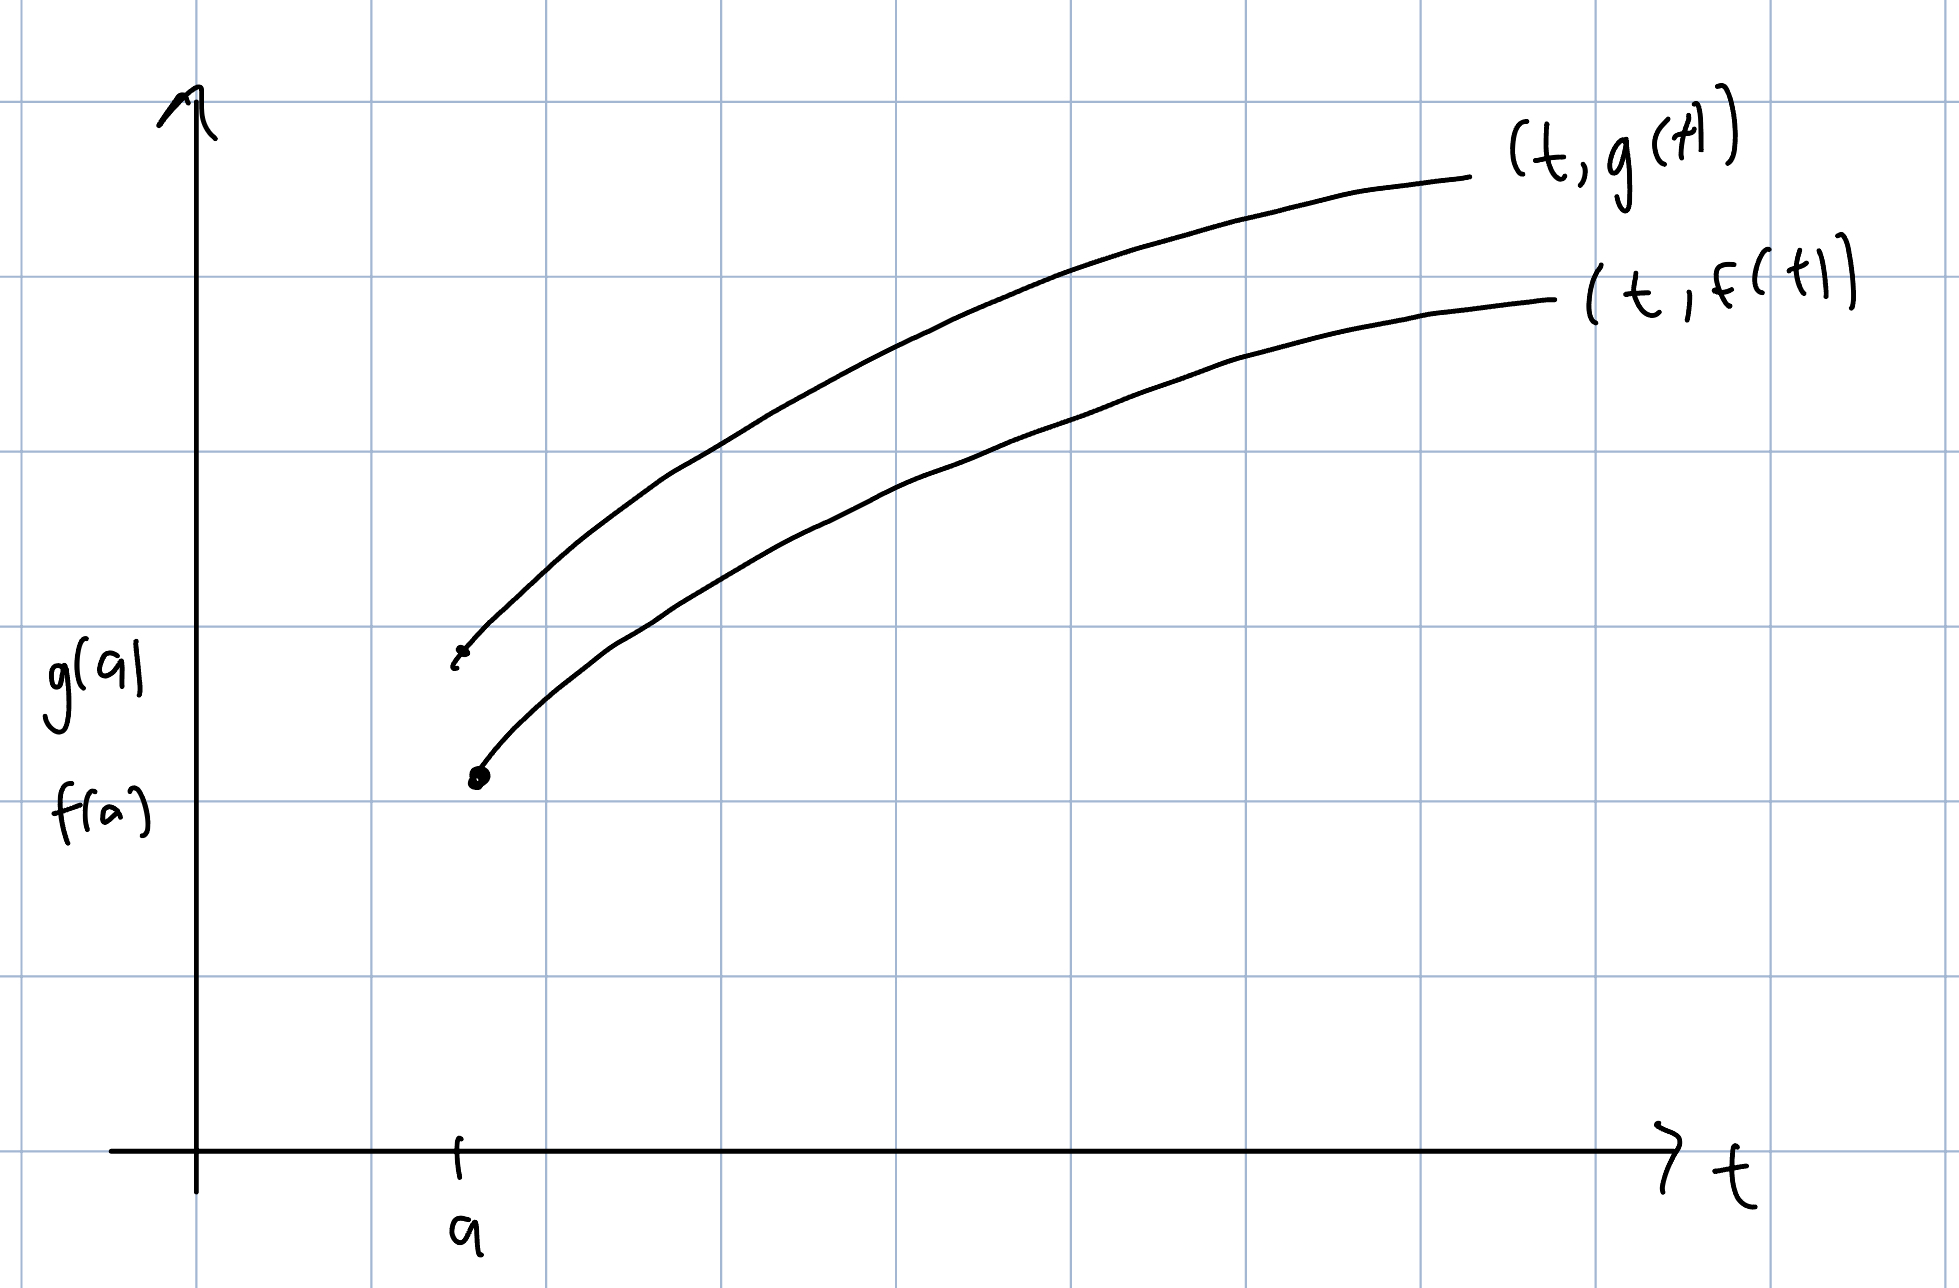
\includegraphics[width=0.6\textwidth]{10-28-1}
		\captionof{figure}{$f$ must be bounded by the known $g$.}
	}
\end{thm}
\begin{proof}
	Suppose for contradiction that there exists $t_1 \in [a,b]$ such that $f(t_1) > g(t_1)$, where $t_1 > a$. 
	Define \[
		\Omega = \{t : f(t) \le g(t)\}
	.\] Note that $\Omega \ne \O$ because $a \in \Omega$. Let \[
	t_0 = \sup \{t \in [a,t_1] \cap  \Omega\}
	.\] 

	(Step 1) We first record what the choice of $t_0$ implies. By definition of $t_0$ as a supremum, we have:
	\begin{align*}
		&\text{(i) } f(t) \le g(t) \quad \text{for all } t \in [a,t_0], \\
		&\text{(ii) } f(t) > g(t) \quad \text{for all } t \in (t_0,t_1].
	\end{align*}

	Since $t_0 = \sup\big( [a,t_1] \cap \Omega \big)$, there exists a sequence
	$t_n \in [a,t_1] \cap \Omega$ with $t_n \to t_0$. For each $n$,
	$f(t_n) \le g(t_n)$, so by continuity of $f$ and $g$,
	\[
		f(t_0) \le g(t_0).
	\]
	On the other hand, by (ii) we have $f(t) > g(t)$ for $t > t_0$ close to $t_0$,
	so continuity again gives
	\[
		f(t_0) \ge g(t_0).
	\]
	Hence
	\[
		f(t_0) = g(t_0).
	\]
	(Step 2) By the first and second assumptions (\ref{10-28-a31}, \ref{10-28-a32}), we get that
	\begin{align*}
		f'(t) - g'(t) &\le F(t,f(t)) - F(t,g(t)) \\
		\implies f(t) - g(t) &\le f(t_0) -g(t_0) + \int_{t_0}^{t} F(s,f(s)) - F(s,g(s))ds \\
		f(t) - g(t) &\le \underbrace{f(t_0) - g(t_0)}_{=0} + \int_{t_0}^{t} F(s,f(s)) - F(s,g(s))ds \\
					&\le \int_{t_0}^{t} L \left| f(s) - g(s) \right|ds \\
					&\le \int_{t_0}^{t} L (f(s) - g(s))ds 
	\end{align*}
	for every $t \in [t_0,t_1]$, since at these values, $f(t) \ge g(t)$.
	Gronwall's inequality gives us $f(t) - g(t) \le 0$ for every $t \in [t_0,t_1]$, which contradicts $f(t_1) - g(t_1) > 0$.
\end{proof}

\section{Thursday, October 30: Comparison, Extension, and Blowup}
\subsection{Comparison}
Suppose we know that
\begin{equation}
	y'(t) \le F(t,y(t)), t \in [a,b] \label{10-30-1}
\end{equation}
We prove the following theorem last class.
\begin{thm}
	Suppose that $F$ is Lipschitz in $y$ such that 
	\begin{align}
		f'(t) &\le F(t,f(t)) \label{10-30a1} \\
		g'(t) &= F(t,g(t)) \label{10-30a2} \\
		\exists f(a) &\le g(a).
	\end{align}
	then $f(t) \le g(t)$ for all $t \in [a,b]$.
\end{thm}

\begin{ex}
	What happens when we have there is no satisfactory Lipschitz $F$? Suppose
	\begin{align*}
		\frac{d}{dt}y &= y^{\frac{1}{3}} \\
		y(0) &= 0 \\
		g &= 0
	.\end{align*}

	Then $y(t) = ct^{\alpha}$ (?) so \[
		\frac{d}{dt}y = c\alpha t^{\alpha-1} = \frac{c_1}{3} t^{\frac{\alpha}{3}}
	.\] Cente $\alpha = \frac{3}{2}$ and $c^{\frac{2}{3}} = \frac{1}{\alpha}$. 
	We get that $C_{\pm} = \pm (\frac{1}{\alpha})^{\frac{3}{2}}$. Then $\left| t \right|^{\frac{3}{2}}$ is a $C^1$ solution to the ODE, but $f$ is then not always less than $g$.
\end{ex}

\begin{thm}
	Suppose
	\begin{align*}
		\frac{d}{dt}x = f(t,x),\quad \frac{d}{dt}y = g(t,y)
	.\end{align*} and we have solutions $x,y$ in the interval $t \in [a,b]$.
	With the assumptions 
	\begin{enumerate}[(i)]
		\item $f(t,z) \le g(t,z), \ \forall  t \in [a,b], z \in D$ 
		\item $f$ or $g$ is locally Lipschitz in $z$ on the region given by $t \in [a,b],z \in D$
		\item $x(a) \le y(a)$.
	\end{enumerate}
	Then $x(t) \le y(t)$ for all $t \in [a,b]$
\end{thm}

\begin{proof}
	We just prove this for if $g$ is Lipschitz. Then 
	\begin{align*}
		\frac{d}{dt}x(t) &= f(t,x) < g(t,x) \\
		\frac{d}{dt} y = g(t,y)	
	.\end{align*}
	We can use the previous theorem.
\end{proof}

\begin{ex}
	Suppose we have a family of ODEs \[
		\frac{d}{dt}x_\alpha(t) = f\left( t,x_\alpha(t) \right) + \alpha 
	\] with the initial conditions \[
		x_\alpha(t_0) = x_0
	.\] Then the functions are increasing in $\alpha$.
\end{ex}

\begin{ex}
	Suppose $\frac{d}{dt}x(t) = P_n(x,t)$ for a polynomial $P_n$. Since $P_n \le c e^x$ eventually, we can use $\frac{d}{dt}y(t) = c e^{y}$ and $y(0) = x_0$ to see that for wherever we can solve $y$, eventually $x(t) \le y(t)$.
\end{ex}

\subsection{Extensibility of Solutions}

Recall the existence-uniqueness theorem:

\begin{thm}
	Given $\frac{d}{dt} x = f(t,x)$ and $x(t_0) = x_0$, some rectangle defined by $\left| t-t_0 \right|<a$, $\left| x-x_0 \right|<b$ on which $f$ is Lipschitz in $x$, and that $f$ is bounded by $M$ on the rectangle, there exists a unique $C^1$ solution for $t \in [t_0-h, t_0+h]$ for \[
		h < \min(\frac{1}{L}, \frac{b}{M}, a)
	.\] 
\end{thm}

This theorem only guarantees a solution in a small neighborhood of $(t_0,x_0)$. 

\begin{ex}
	(Blowup) Consider $\frac{d}{dt} y = y^2$ and $y(0) = 1$. The solution is given by \[
		y(t) = \frac{1}{1-t}
	\] in a neighborhood. However, \[
		\lim\limits_{t \to 1^-} y(t) = \infty
	,\] so we say this solution exists up to $1^-$.
\end{ex}

How can we characterize $(t^-, t^+)$ where the solution exists?

\begin{lemma}
	(Gluing Lemma) Suppose $f(t,x(t)) \in C(\R \times \R)$ and Lipschitz with respect to a function $L_D$ in $x$ in any bounded region $D$ such that $L_D$ is bounded on $D$. Suppose $\phi_i(t)$ solves \[
		\frac{d}{dt}\phi_i(t) = f(t,\phi(t)), \phi(t_0) = x_0
	\] when $t \in I_i (a_i,b_i)$ for $i \in \{1,2\}$.

	If $t_0 \in I_1 \cap I_2$ and \[
		\phi_1(t_0) = \phi_2(t_0)
	,\] then \[
		\phi_1(t) = \phi_2(t)
	\] for $t \in I_1 \cap  I_2$ and \[
		\phi(t) = \begin{cases}
			\phi_1(t),\quad t \in I_1 \\
			\phi_2(t), \quad t\in I_2
		\end{cases}
	\] is a $C^1$ solution to the ODE on $I_1 \cup I_2$.
\end{lemma}

\begin{proof}
	Apply the existence-uniqueness theorem to \[
		\frac{d}{dt}x(t) = f(t,x(t)), \quad x(t_0) = x_0
	.\] There exists a unique $C^1$ solution $x(t)$ on some interval $[t_0-h,t_0+h]$. By uniqueness, $\phi_1(t) = \phi_2(t)$ for $t \in [t_0-h,t_0+h] =: [a,b]$.

	Define \[
		J^- = \{p : \phi_1(t) = \phi_2(t), t \in [p,t_0+h] \cap (a,b) \}
	.\] Define \[
		A = \inf J^-
	.\]
	We want to show that $A = a$.

	(Method 1) Define $J = \{t \in I_1 \cap I_2 : \phi_1(t) = \phi_2(t)\}$. $J$ is relative closed (by continuity) and relative open (by step 1). It is nonempty, so $J = I_1 \cap  I_2$.

	(Method 2) By definition of infimum, there exists a sequence $\{p_n\} \subset J^-$ that converges to $A$. Suppose for contradiction that $A > a$. By definition of $J^-$, for each $n \in \N$, \[
		\phi_1(p_n) = \phi_2(p_n)
	.\] Sending $n \to \infty$, \[
		\phi_1(A) = \phi_2(A)
	,\] so $A = a$. 
	Using existence-uniqueness, we can replace $(t_0,x_0)$ with $(A, \phi_1(A))$ so $\phi_1(t) = \phi_2(t)$ for $t \in [A-h, A+h]$, contradicting $A$ being the infimum of $J^-$. The two solutions must agree at the end endpoint (and we can reproduce it with $\sup$ to extend to $b$).

	Now we know that $\phi_1$ and $\phi_2$ agree on $[a,b]$. $\phi$ as given below is well-defined: \[
		\phi(t) = \begin{cases}
			\phi_1(t), \quad t \in I_1 \\
			\phi_2(t),\quad t\in I_2
		\end{cases}
	.\] $\phi$ is $C^1 (I_1 \cup I_2)$. It is also a solution to the ODE $\phi' = f(t,\phi)$, as \[
		\begin{cases}
			\phi'(t) = \phi_1'(t) = f(t,\phi_1) = f(t,\phi), \quad t \in I_1 \\
			\phi'(t) = \phi_2'(t) = f(t,\phi_2) = f(t,\phi), \quad t \in I_2
		\end{cases}
	.\] 

\end{proof}

\section{Thursday, November 6: Extension and Blowup}

\subsection{Review}

Consider \[
	\frac{d}{dt}x = f(t,x(t))
,\] where $f \in C(R \times R)$ and $f$ is Lipschitz in its second argument in any bounded domain $D$.\marginnote{Note that this is automatically implied if $\frac{\partial f}{\partial y}$ exists.} These assumptions will hold for the entirety of this lecture.

Recall the gluing lemma:\marginnote{An alternative proof uses Gronwall's inequality with \[
	\left| \phi_1(t) - \phi_2(t) \right| \le \int_{t_0}^{t} L_D \left| \phi_1(s) - \phi_2(s) \right|ds 
\] for $t \in I_1 \cap I_2$ to prove the first, trickier part of the lemma result.}
\begin{lemma}
	Suppose that $\phi_i(t)$ solves the ODE, $I_i = (a_i,b_i)$, and $t_0 \in I_1 \cap I_2 = (a,b) \ne \O$.

	If $\phi_1(t_0) = \phi_2(t_0)$, then \[
		\phi_1(t) = \phi_2(t)
	\] for $t \in I_1 \cap I_2$, so we can define \[
		\phi(t) = \begin{cases}
			\phi_1(t), \quad t \in I_1, \\
			\phi_2(t), \quad t \in I_2
		\end{cases}
	\] for $t \in I_1 \cup I_2$, where $\phi$ is the unique $C^1$ solution to the ODE.
\end{lemma}

Now we wonder what happens if $f$ is not Lipschitz but we have two solutions in overlapping domains. By drawing a picture, the first conclusion is not true, while $\phi$ in the second conclusion is not well-defined. There are multiple choices for how to glue $\phi_1$ and $\phi_2$ together.

\subsection{Blowup}

\begin{thm} \label{thm:blowup}
	(Blowup Criterion for Extension) Suppose that \[
		\frac{d}{dt}\phi(t) = f(t,\phi(t))
	\] for $t \in (t_-, t_+)$, where $f \in C(\R\times \R)$ and $f$ is Lipschitz in its second argument. The solution can extend to $\left( t_-, t_+ + \epsilon \right)$ for some $\epsilon > 0$ if and only if there exists a sequence $\{t_n\}$ such that \[
		t_n \to \left( t_+ \right)^-, \qquad \phi(t_n) \to \phi_0 \in \R
	.\]We can also write this as \[
	(t_n, \phi(t_n)) \to (t_+, \phi_0)
	.\] Alternatively, the solution extends if and only if \[
		\liminf\limits_{t \to \left( t_+ \right)^{-}} \left| \phi(t) \right| < \infty
	.\] 
\end{thm}

We can reformulate the theorem to get 
\begin{thm}
	(Blowup Criterion for Extension, Alternative) $\phi(t)$ cannot extend beyond $t_+$ if and only if \[
		\lim\limits_{t \to \left( t_+ \right)^{-}} \left| \phi(t) \right| = \infty
	.\] 
\end{thm}

\begin{proof}
	(Of Theorem (\ref{thm:blowup})) Since $\phi$ is continuous, extensibility implies that the limit as $t \to t_+$ from the left is exists and is finite (in fact, equal to $\phi(t_+)$, so the forwards direction is immediate.

	For the backwards direction, suppose there exists a sequence $\{t_n\}$ \[
		\left( t_n, \phi(t_n) \right) \to (t_+, \phi_0)
	.\] 

	Then there exists $N \in \N$ such that for $n \ge N$, \[
		\left| \phi(t_n) - \phi_0 \right| \le 1
	.\] We want to use existence-uniqueness to get a $\phi_{new}(t)$ that solves the ODE on some open interval that contains $t_+$.

	(Step 1) First define \[
		D = \left[ t_+ -2, t_+ + 2 \right] \times \left[ \phi_0-2,\phi_0+2 \right] 
	.\] By the two assumptions, \[
		\left| f \right| \le M \text{ in } D, \qquad \left| f(t,x) - f(t,y) \right| \le L \left| x-y \right|
	.\] Importantly, $M$ and $L$ are independent of $n$; they only depend on the accumulation point. 

	(Step 2) We apply existence-uniqueness with the initial condition $(t_n, \phi(t_n))$ to get a solution \[
		\phi_{new}(t_n) = \phi(t_n)
	\] for $t \in (t_n -h, t_n+ h)$, where \[
		h < \frac{1}{2} \min \{1, \frac{1}{M}, \frac{1}{L}\}
	.\] Again, we see that $h$ is independent of $n$ --- in particular, as $n\to \infty$, $h$ remains positively bounded above $0$.

	(Step 3) Hence, we can pick $n$ large enough such that \[
		t_n + h > t_+
	.\] We have two solutions \[
		\begin{cases}
			\phi_{new}(t), \quad &t \in (t_n - h, t_n + h) \\
			\phi(t), \quad &t \in (t_-, t_+)
		\end{cases}
	\] that both solve the ODE and coincide with $\phi(t_n) = \phi_{new}(t_n)$, so we can use the gluing lemma to extend $\phi$ to be defined on \[
	(t_-, t_n+h) \subseteq \left( t_-, t_+ \right) \cup \left( t_n - h, t_n+ h \right)
	,\] where $t_+ + \epsilon$ is contained in the interval.
\end{proof}

A crucial part of the proof was noting that $f$ is bounded and Lipschitz in some large region, then solving the ODE on a smaller subregion so $\phi_{new}$ is within the large region.\marginnote{\texthl{why?}}

A priori, we could not exclude an oscillation near the limiting point, but after completing the proof, we know that the solution $\phi$ is $C^1$.\marginnote{how can $\phi$ wildly oscillate if $\phi' = f$ is bounded by $M$??\texthl{??}}

\subsection{Global Solutions}
What kinds of ODEs have global solutions? Can we think of any that we cannot solve by hand? This question may seem ill-posed, but we can actually answer it using the blowup criterion.

Suppose \[
	\frac{d}{dt}x = f(t,x)
,\] where $\left| f \right| < M$; i.e., $f$ is uniformly bounded. We claim that this ODE has a unique (up to initial condition (?)) global $C^1$ solution.

Supposing not, in that we only have a solution on $(t_-, t_+)$, we get
\begin{align*}
	\left| x(t) - x(t_0) \right| &= \left| \int_{t_0}^{t} f(s, x(s))ds  \right| \\
								 &\le M \left| t-t_0 \right| < \infty
.\end{align*} We get that any sequence $\{t_n\} \to t_+$ has a subsequence such that $\{x(t_n)\}$ converges, so $x$ extends by the blowup criterion.

\subsection{Finite-time Blowup}
Finite-time blowup means that the derivative of the solution goes to infinity near some point; it is the opposite of existence of a global solution.

Suppose we have \[
	\frac{d}{dt} y = y^p, \qquad y(0) = 1
.\] When $p= 1$, $y(t) = e^t$.

Consider when $p>1$. Because $y(0) > 1$, we know that $y^p \ge y$. Using separation of variables,
\begin{align*}
	\frac{\frac{d}{dt}y}{y^p} &=  1 \\
	\implies y^{1-p}(t) &= 1 + (1-p)t \\
	y^{p-1}(t) &= \frac{1}{\underbrace{1-(p-1)t}_{>0}}
,\end{align*}
so $y^{p-1}(t) \to \infty$ as $t \to \frac{1}{p-1}$.
We see that with faster-than-exponential growth, the solution goes to $\infty$ in finite time, so $p=1$ is a borderline case.


Recall from comparison that if \[
	\frac{d}{dt}x = f(t,x), \qquad \frac{d}{dt}y = g(t,y)
,\] where \[
	f \le g, \qquad x(0) < y(0)
,\] we know that \[
	x(t) \le y(t)
\] for $t \in I_x \cap I_y$.

\begin{ex}
	Consider \[
		\frac{d}{dt} y = e^{y}
	.\] By comparison ($e^{y} \ge y^2$), we see that there does not exist a global solution. The same thing applies to the ODE \[
		\frac{d}{dt}y = y^{n} + \ldots+1 + e^t
	\] for $n \ge 2$.
\end{ex}

\begin{ex}
	Consider \[
		\frac{d}{dt}y = y^2, \qquad y(0) = y_0
	.\] If $y_0 = 0$, then $y = 0$. If $y_0 > 0$, then we see blowup as $t \to \infty$. If $y_0 < 0$, we get the solution formula \[
		y(t) = \frac{y_0}{1-t y_0} \sim -\frac{1}{t}
	.\] So, $y$ starts below $0$ then increases to $0^-$ as $t \to \infty$.

	This ODE is interesting; a small perturbation from $y_0$ in the positive direction leads to a large change in the solution (we now have blowup), but a perturbation in the negative direction leads to equivalent behavior in the distant horizon.
\end{ex}

\begin{ex}
	What if we now perturb with \[
		\frac{d}{dt} y = y^2 + \epsilon, \qquad y(0) = y_0
	?\] 
	Since \[
		y(t) \ge y_0 + \epsilon t
	,\] which is eventually positive, we see that $y(t_0) > 0$ for $t_0$ large. Hence \[
		\frac{d}{dt} y \ge y^2
	,\] so we have blowup.
\end{ex}

\begin{ex}
	If we have \[
		\frac{d}{dt}y = y^2 - \epsilon^2, \qquad y_0 \in (-\epsilon, \epsilon)
	,\] we get very different behaviors around $-\epsilon, \epsilon$.
\end{ex}

\section{Blowup Criterion, Redone}

\subsection{Blowup}

\begin{defn}[Maximal solution]
	Let $f \colon \R \times \R \to \R$ be continuous and locally Lipschitz in its second argument.
	A solution $\phi \colon I \to \R$ of
	\[
		\phi'(t) = f(t,\phi(t))
	\]
	on an interval $I \subset \R$ is called \emph{maximal} if there is no strictly larger interval
	$J \supsetneq I$ and solution $\tilde\phi \colon J \to \R$ such that
	$\tilde\phi(t) = \phi(t)$ for all $t \in I$.
\end{defn}

\begin{thm}[Blowup criterion]\label{thm:blowup}
	Consider the IVP
	\[
		\phi'(t) = f(t,\phi(t)), \qquad t \in (t_-,t_+),
	\]
	where $f \in C(\R \times \R)$ and $f$ is locally Lipschitz in its second argument.
	Let $\phi \colon (t_-,t_+) \to \R$ be a solution.

	Then the following are equivalent:
	\begin{enumerate}[(i)]
		\item $\phi$ extends to a solution on a larger interval
		      $(t_-,t_+ + \varepsilon)$ for some $\varepsilon > 0$;
		\item there exists a sequence $t_n \in (t_-,t_+)$ with
		      \[
		      	t_n \to t_+^{-}, \qquad \phi(t_n) \to \phi_0 \in \R,
		      \]
		      i.e.\ the graph $(t_n,\phi(t_n))$ has a finite limit point $(t_+,\phi_0)$;
		\item 
		      \[
		      	\liminf_{t \to t_+^{-}} |\phi(t)| < \infty.
		      \]
	\end{enumerate}
\end{thm}

\begin{rmk}
	Geometrically, we are looking at the curve $t \mapsto (t,\phi(t))$ in the $(t,x)$–plane.
	The theorem says:
	\marginnote{If the solution does not ``run off to infinity'' in finite time,
	then its graph accumulates at some finite point $(t_+,\phi_0)$, and from that
	point we can restart the IVP and continue the solution a bit further in $t$.}
	the solution can be continued a little past $t_+$ if and only if, as
	$t \to t_+^{-}$, the curve stays inside some vertical strip
	$\{(t,x) : t < t_+, |x| \le R\}$.
	The only obstruction to continuation is that $|\phi(t)|$ blows up in finite time.
\end{rmk}

\begin{proof}
	We will prove (i) $\Leftrightarrow$ (ii), and then see that (ii) $\Leftrightarrow$ (iii)
	is just a basic fact about $\liminf$.

	\medskip

	\noindent\emph{(i) $\Rightarrow$ (ii).}
	Suppose $\phi$ extends to a solution on $(t_-,t_+ + \varepsilon)$ for some $\varepsilon > 0$.
	Denote this extension by $\tilde\phi \colon (t_-,t_+ + \varepsilon) \to \R$, so
	$\tilde\phi(t) = \phi(t)$ for $t \in (t_-,t_+)$ and $\tilde\phi$ satisfies
	\[
		\tilde\phi'(t) = f(t,\tilde\phi(t))
	\]
	for all $t \in (t_-,t_+ + \varepsilon)$.
	Since $\tilde\phi$ is continuous, the one–sided limit
	\[
		\tilde\phi(t_+) = \lim_{t \to t_+} \tilde\phi(t)
	\]
	exists and is finite.

	Now fix any sequence $t_n \in (t_-,t_+)$ with $t_n \to t_+^{-}$. Then
	\[
		\phi(t_n) = \tilde\phi(t_n) \to \tilde\phi(t_+) = \phi_0,
	\]
	which is exactly condition (ii).

	\medskip

	\noindent\emph{(ii) $\Rightarrow$ (iii).}
	If we have $t_n \to t_+^{-}$ and $\phi(t_n) \to \phi_0 \in \R$, then the sequence
	$\{ \phi(t_n) \}$ is bounded.
	By definition of the liminf,
	\[
		\liminf_{t \to t_+^{-}} |\phi(t)|
		\;\le\; \lim_{n \to \infty} |\phi(t_n)|
		= |\phi_0| < \infty,
	\]
	so (iii) holds.

	\medskip

	\noindent\emph{(iii) $\Rightarrow$ (ii).}
	This is a purely real–analysis statement: for any real–valued function $g$,
	\[
		\liminf_{t \to t_+^{-}} |g(t)| < \infty
		\quad \Longleftrightarrow \quad
		\exists \, t_n \to t_+^{-} \text{ with } |g(t_n)| \text{ bounded.}
	\]
	Applying the Bolzano–Weierstrass theorem to the bounded sequence $\{g(t_n)\}$,
	we can pass to a subsequence (which we still call $t_n$) such that $g(t_n)$ converges.
	Applied to $g = \phi$, this gives exactly (ii).

	\medskip

	\noindent\emph{(ii) $\Rightarrow$ (i).}
	This is the nontrivial direction: we show that if the solution has a finite
	limit point at $t_+$, then it can be extended beyond $t_+$.

	Assume there exists a sequence $t_n \to t_+^{-}$ such that
	\[
		\phi(t_n) \to \phi_0 \in \R.
	\]
	Consider the point $(t_+,\phi_0)$ in the $(t,x)$–plane. Since $f$ is continuous and
	locally Lipschitz in $x$, there is a closed rectangle
	\[
		Q: [t_+ - a,\, t_+ + a] \times [\phi_0 - b,\, \phi_0 + b]
	\]
	with $a,b>0$ such that:
	\begin{enumerate}[(1)]
		\item $f$ is bounded on $Q$, say $|f(t,x)| \le M$ for all $(t,x) \in Q$;
		\item $f$ is Lipschitz in $x$ on $Q$ with some constant $L$.
	\end{enumerate}
	\marginnote{We are using here the quantitative version of the
	existence–uniqueness theorem: on any compact rectangle where $f$ and its Lipschitz
	constant are bounded, we get a uniform existence time $h>0$ for all initial values
	in a slightly smaller rectangle.}

	By the usual proof of the Picard–Lindelöf theorem, there exists $h>0$ (depending
	only on $a,b,M$) such that for every $(s,x) \in Q$ there is a unique solution
	$y(\,\cdot\,;s,x)$ of
	\[
		y'(t) = f(t,y(t)), \qquad y(s) = x,
	\]
	defined at least on the interval $[s-h,s+h] \subset (t_+ - a, t_+ + a)$.

	In particular:
	\begin{itemize}
		\item there is a unique solution $\psi$ with
		      \[
		      	\psi'(t) = f(t,\psi(t)), \qquad \psi(t_+) = \phi_0,
		      \]
		      defined on $(t_+ - h,t_+ + h)$;
		\item for all $n$ large enough, $(t_n,\phi(t_n)) \in Q$,
		      so there is a unique solution $\psi_n$ with
		      \[
		      	\psi_n'(t) = f(t,\psi_n(t)), \qquad \psi_n(t_n) = \phi(t_n),
		      \]
		      defined on $(t_n - h,t_n + h)$.
	\end{itemize}

	Now note:
	\begin{itemize}
		\item Since $\phi$ is already a solution with $\phi(t_n) = \psi_n(t_n)$,
		      uniqueness gives
		      \[
		      	\psi_n(t) = \phi(t)
		      	\qquad\text{for all } t \in (t_-,t_+) \cap (t_n - h,t_n + h).
		      \]
		      In particular, for $n$ large enough we have
		      \[
		      	\psi_n(t) = \phi(t)
		      	\qquad\text{for all } t \in (t_+ - h/2, t_+).
		      \]
		\item The continuous dependence of solutions on initial data
		      (proved earlier via Gronwall) says that if
		      $(t_n,\phi(t_n)) \to (t_+,\phi_0)$, then
		      \[
		      	\psi_n \to \psi
		      	\quad\text{uniformly on any compact subinterval of } (t_+ - h,t_+ + h).
		      \]
	\end{itemize}

	Fix a compact interval $[t_0,t_+] \subset (t_+ - h,t_+)$.
	For $n$ large enough, we have $\psi_n(t) = \phi(t)$ on $[t_0,t_+]$, and
	$\psi_n \to \psi$ uniformly on $[t_0,t_+]$. Hence
	\[
		\psi(t) = \lim_{n\to\infty} \psi_n(t)
		= \lim_{n\to\infty} \phi(t)
		= \phi(t)
		\qquad\text{for all } t \in [t_0,t_+).
	\]
	Since $t_0$ was arbitrary in $(t_+ - h,t_+)$, this shows
	\[
		\psi(t) = \phi(t)
		\qquad\text{for all } t \in (t_+ - h,t_+).
	\]

	Thus $\psi$ is an honest extension of $\phi$ beyond $t_+$:
	define
	\[
		\widetilde\phi(t) =
		\begin{cases}
			\phi(t), & t \in (t_-,t_+), \\
			\psi(t), & t \in [t_+, t_+ + h).
		\end{cases}
	\]
	Then $\widetilde\phi$ is $C^1$ on $(t_-,t_+ + h)$, satisfies
	$\widetilde\phi'(t) = f(t,\widetilde\phi(t))$ for all
	$t \in (t_-,t_+ + h)$, and extends $\phi$ to the larger interval
	$(t_-,t_+ + h)$.
	This is exactly (i).

	\medskip

	We have now shown (i) $\Leftrightarrow$ (ii) and (ii) $\Leftrightarrow$ (iii),
	so all three statements are equivalent.
\end{proof}

\begin{thm}[Blowup criterion, alternative form]\label{thm:blowup-alt}
	Let $\phi \colon (t_-,t_+) \to \R$ be a maximal solution of
	\[
		\phi'(t) = f(t,\phi(t)),
	\]
	with $f$ as above, and suppose $t_+ < \infty$.
	Then $\phi$ \emph{cannot} be extended beyond $t_+$ if and only if
	\[
		\lim_{t \to t_+^{-}} |\phi(t)| = \infty.
	\]
	In other words, finite–time breakdown of a maximal solution can only occur
	by blowup of the solution itself.
\end{thm}

\begin{proof}
	Since $\phi$ is maximal and $t_+ < \infty$, by definition it cannot be extended
	past $t_+$. By Theorem~\ref{thm:blowup}, this means that
	\[
		\liminf_{t \to t_+^{-}} |\phi(t)| = \infty.
	\]
	But $\liminf_{t\to t_+^{-}} |\phi(t)| = \infty$ is equivalent to
	\[
		\forall M > 0 \;\exists \delta > 0 \;\text{such that}\;
		t_+ - \delta < t < t_+ \implies |\phi(t)| > M,
	\]
	which is exactly the statement that $|\phi(t)| \to \infty$ as $t \to t_+^{-}$,
	i.e.\ $\lim_{t\to t_+^{-}} |\phi(t)| = \infty$.

	Conversely, if $|\phi(t)| \to \infty$ as $t \to t_+^{-}$ but $\phi$ could
	be extended to a larger interval $(t_-,t_+ + \varepsilon)$, the extension would
	be continuous on a compact interval $[t_+ - \varepsilon/2,t_+]$ and hence bounded
	there, contradicting $|\phi(t)| \to \infty$.
\end{proof}

\begin{rmk}
	There is a completely analogous statement at the left endpoint $t_-$: if the
	maximal solution has $t_- > -\infty$, then $\phi$ cannot be extended to the left
	if and only if $|\phi(t)| \to \infty$ as $t \to t_-^{+}$.
\end{rmk}

\section{Autonomous ODEs, Stability}
\subsection{Preliminaries}
\begin{defn}[Autonomous ODE]
	An autonomous ODE is one we can write in the form \[
		\frac{d}{dt} \vec x = F(\vec x)
	.\] In other words, $\frac{d}{dt} \vec x$ does not depend on $t$.
\end{defn}

With an autonomous ODE, if we find a point $x^*$ at which $F(x^*) = 0$, we get that the unique solution to the ODE is a constant. We refer to $x^*$ as a critical point.

\begin{defn}[Trajectory]
	The trajectory of an ODE is the curve defined by $(t,X(t))$.
\end{defn}

When $X(t) \in R^2$, we can think of $x_2$ as a function of $x_1$\footnote{As long as $X' = \left( x_1',x_2' \right) \ne 0$} by the implicit function theorem.
Varying $t$, we can plot $x_2$ against $x_1$ to get a graph in the \emph{phase plane}: the $x_1$$x_2$ - plane.

\begin{defn}[Phase portrait]
	The representative set of a trajectory is called the phase portrait. By representative set, we mean the set of all trajectories attained by varying $x_{1,0}$ and $x_{2,0}$.
\end{defn}

\begin{ex}
	Consider the autonomous ODE $\frac{d}{dt}x = x^2- x$. We want to set $f = x^2 - x = 0$, so our critical points are \[
		x = 0, \qquad x = 1
	.\] Then we have two special solutions $x_1(t) = 0$ and $x_2(t)=1$.
\end{ex}

\begin{ex}
	Now consider the autonomous ODE system \[
		\begin{cases}
			\frac{d}{dt}x = x^2 - 2y \\
			\frac{d}{dt}y = x + y
		\end{cases}
	.\] Setting them equal to 0, we get the system \[
		x^2 = 2y, \qquad x = -y
	.\] Hence our two critical points are \[
	(x,y) = (0,0), \quad (-2, 2)
	.\] 
\end{ex}

\subsection{Linear $2\times 2$ System}

In this section, consider $\frac{d}{dt} X = AX$, where $A \in \R^{2\times 2}$.

Note that we have an equilibrium for $X$ being the eigenvector associated with an eigenvalue of $0$; i.e., the kernel of $A$.

In general, if $Av_i = \lambda_i v_i$, we have the solution \[
	x(t) = c_1e^{\lambda_1 t}v_1 + c_2 e^{\lambda_2 t}v_2
.\] Recall the three cases we have:
\begin{enumerate}[(I)]
	\item $\lambda_1 < \lambda_2$ and are both real,
	\item $\lambda_1 = \overline{\lambda_2}$, and
	\item $\lambda_1=\lambda_2$ is real.
\end{enumerate}

\newthought{In case (I)} , we can write the general solution as 
\marginnote{
	\begin{center}
		
\includegraphics[width=0.5\textwidth]{11-11-1}
		\captionof{figure}{Case (I)}
	\end{center}
}
\[
	x(t) = e^{\lambda_2 t} \left( e^{(\lambda_1 - \lambda_2) t}c_1v_1 + c_2v_2 \right)
.\] When $\lambda_1 < \lambda_2 < 0$, we see that if either $c_1=0$ or $c_2=0$, then $x$ goes to $0$ as time goes to $\infty$: \[
x_1(t) = c_1 e^{\lambda_1 t} v_1 \xrightarrow{t \to \infty} 0
.\] Similarly, \[
	x_2(t) = c_2e^{\lambda_2 t} v_2 \xrightarrow{t\to \infty} 0
\] by putting $c_1 = 0$. If $c_1,c_2 \ne 0$, then we look at the general solution and see that since $\lambda_1 < \lambda_2$, the first term inside the parentheses goes to $0$. Hence the asymptotic behavior is like $e^{\lambda_2 t} \left( c_2v_2 \right)$, which goes to $0$.

When $\lambda_1 < 0 < \lambda_2$, we see that $x_1 \to 0$ but $x_2$ goes to either $\infty$ or $-\infty$, depending on the sign of $c_2$. The asymptotic behavior of $x$ has not changed: $x(t) \approx e^{\lambda_2 t} c_2 v_2$. Hence, $x(t) \to 0$ iff $c_2 = 0$.


When $0 < \lambda_1 < \lambda_2$, both $x_1$ and $x_2$ go to $\infty$ or $-\infty$. Again, the asymptotic behavior is the same, so $x(t) \to 0$ iff $c_1 = 0$.

\newthought{In case (II)}, write
\begin{align*}
	\lambda_{\pm} &= \alpha \pm i \beta \\
	v_{\pm} &= \alpha \pm i b
.\end{align*}
\marginnote{
	\begin{center}
		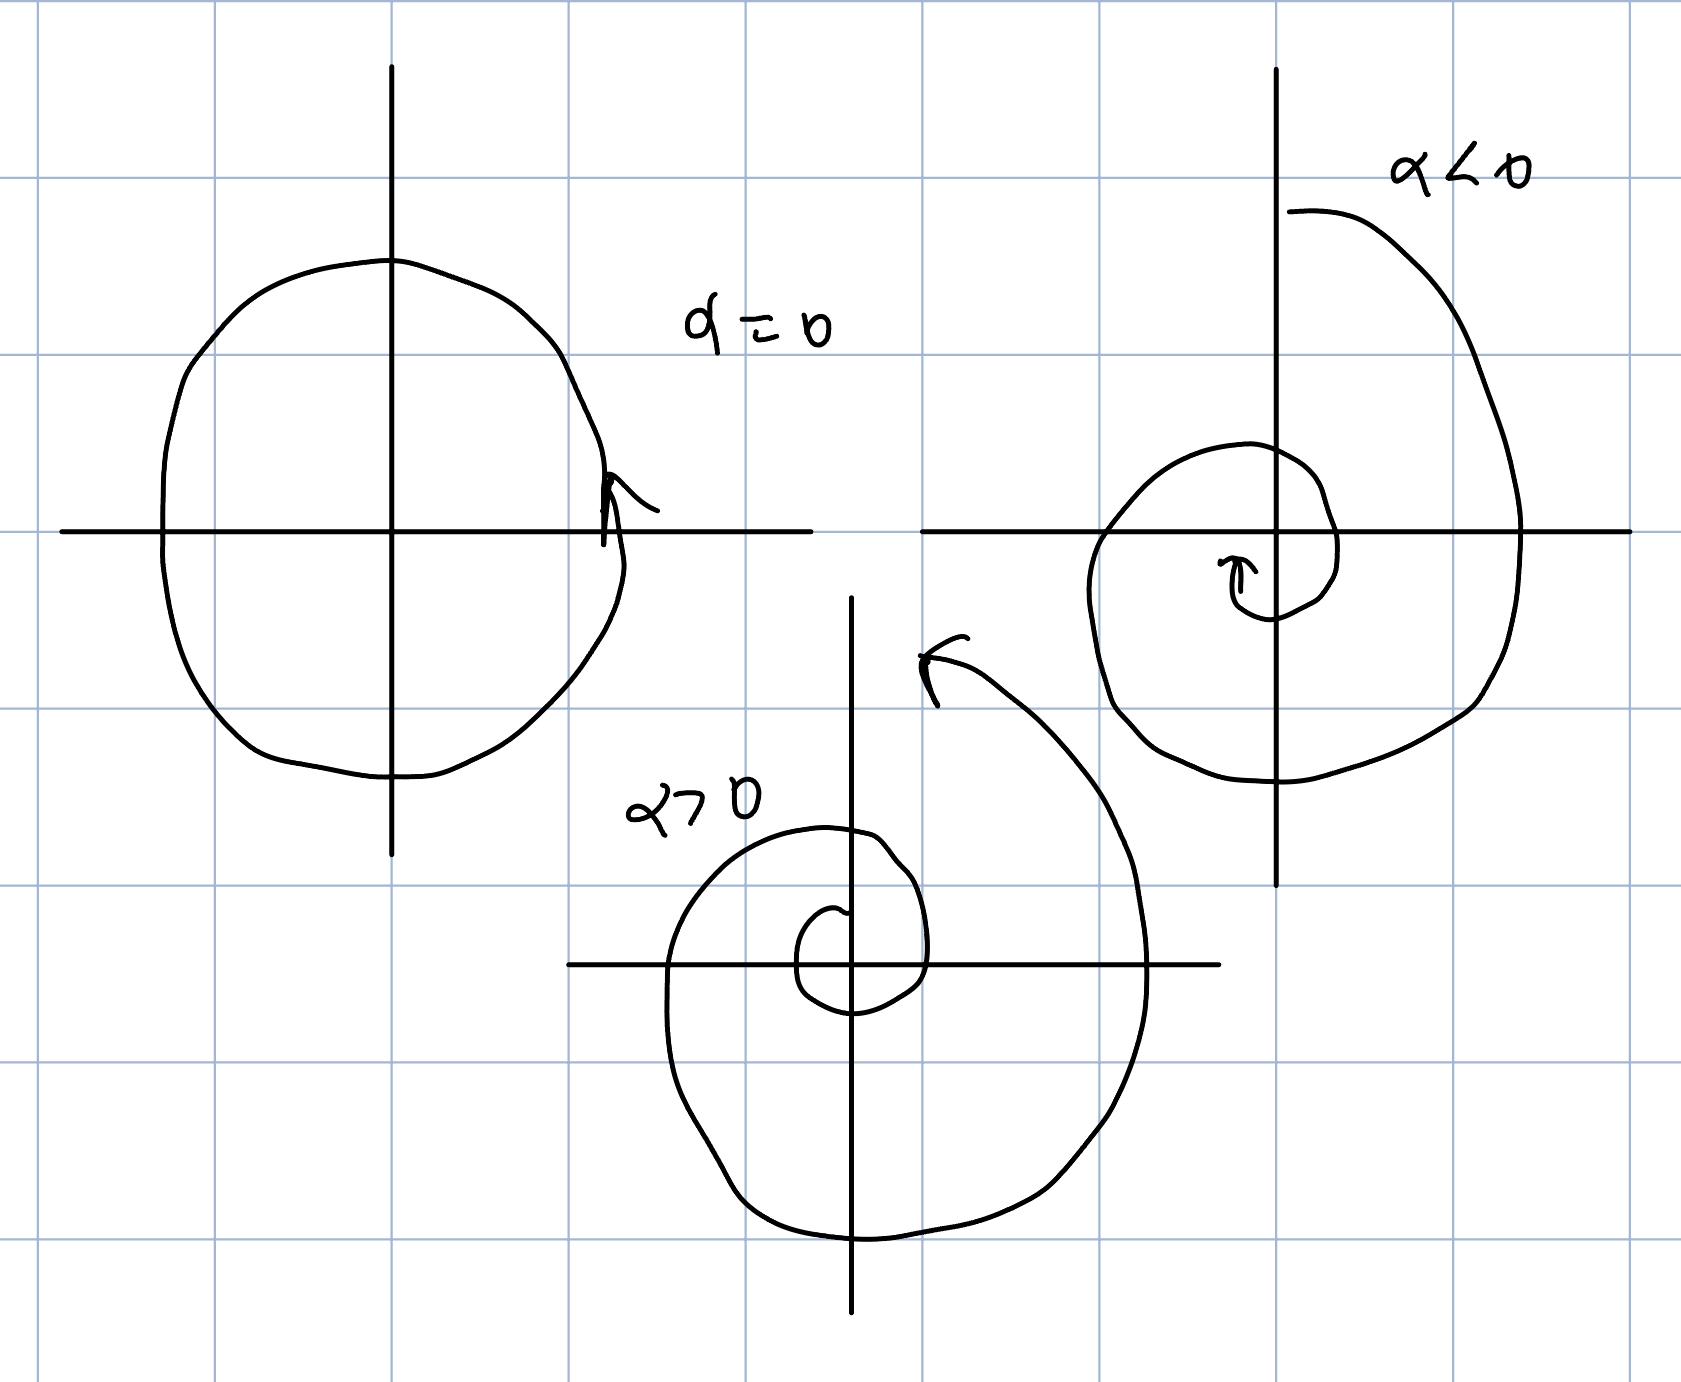
\includegraphics[width=0.5\textwidth]{11-11-2}
		\captionof{figure}{Case (II)}
	\end{center}
}
Then 
\begin{align*}
	x(t) &= c_1 \text{Re} \left( e^{\lambda_+ t}v_+ \right) + c_2 \text{Im} \left( e^{\lambda_+}v_+ \right) \\
		 &= e^{\alpha t} \left[ c_1 (\cos{\left(\beta t\right)} a - \sin{\left(\beta t\right)}b \right] + c_2 \left( \sin{\left(\beta t\right)} a + \cos{\left(\beta t\right)}b \right) \\
		 &= e^{\alpha t} v(t)	
.\end{align*}
We see that $\left| x \right|$ has the behavior \[
	\begin{cases}
		\left| x(t) \right| \to \infty, \quad \alpha > 0 \\
		\left| x(t) \right|= 1,\qquad\alpha = 0 \\
		\left| x(t) \right| \to 0, \qquad \alpha<0
	\end{cases}
.\] 

\newthought{In case (III)}, we have $\lambda_1 = \lambda_2 = \lambda$. When we have two distinct eigenvectors $v_1,v_2$, we can write \[
	x(t) = e^{\lambda t} \underbrace{\left( c_1v_1 + c_2v_2) \right)}_{\text{constant}}
.\] Hence, the trajectory is affine and depending on if $\lambda < 0$, $\lambda = 0$, or $\lambda > 0$, we see that we either $(0,0)$ is a source, sink, or the trajectory is just constant at the initial point.

When we have one eigenvector and one generalized eigenvector, we have to write \[
	x(t) = e^{\lambda t} (c_1v_1 + c_2 t v_2)
,\]  and the term in the parentheses is no longer constant. But as we send $t \to \infty$, eventually the direction becomes that of $v_2$: \[
	x(t) = e^{\lambda t} t \left( \frac{1}{t}c_1v_1 + c_2v_2 \right)
.\] Then the trajectory depends on $\lambda$ and differs from when he had two distinct eigenvectors for the $\lambda = 0$ case: \[
	\begin{cases}
		\left| x(t) \right| \to \infty \text{ exponentially}, \quad \lambda > 0 \\
		\left| x(t)  \right| \to \infty \text{ linearly}, \quad \lambda = 0 \\
		\left| x(t) \right| \to 0 \text{ exponentially}, \quad \lambda < 0
	\end{cases}
.\] 

\begin{aside}
	If we write $x_2 = x_2\left( x_1 \right)$, how smooth is $x_2 \in C^k$, where $x_2 \not\in C^{k + \epsilon}$?
\end{aside}

\subsection{Nonlinear Systems}
Drawing phase portraits for nonlinear systems is hard. Consider $f_1,\ f_2$ polynomials and
\begin{align*}
	\frac{d}{dt}x_1 &= f_1(x_1,x_2; b) \\
	\frac{d}{dt}x_2 &= f_2(x_1,x_2; b)
.\end{align*}

We have a critical point $(0,0)$ and other critical points $X_c$ that are functions of the parameters.

Can we find a trajectory and parameter $b$ that connects $(0,0)$ to $X_c$ in a $C^{\infty}$ way? That's a hard problem. It relates to having \[
	\frac{dx_2}{dx_1} = \frac{f_1}{f_2}
,\] trying to solve with a degenerate point, then running into trouble because the function is not Lipschitz.

\subsection{Linear Stability}
\begin{defn}[Stable solution]
	We say that the ODE is stable at $x^*$ if for every $\epsilon > 0$, there exists $\delta > 0$ such that for any $x_0$, \[
		\left| x_0 - x^* \right| < \delta \implies \left| x(t) - x^* \right| < \epsilon
	\] for every $t \ge t_0$. In other words, if we start close to the point at which the ODE is stable, it stay within an $\epsilon$-ball forever.
	$x^*$ is unstable if it is not stable.
\end{defn}

\begin{defn}[Asymptotically stable solution]
	We say that $x^*$ is an asymptotically stable solution to the ODE if for every $\epsilon > 0$, there exists $\delta > 0$ such that \[
		\left| x_0 - x^* \right| < \delta \implies \lim\limits_{t \to \infty} x(t) = x^*
	\] for every $t \ge t_0$.
\end{defn}

Asymptotic stability implies stability. Stability allows for very small oscillations in the limit, while asymptotic stability requires convergence.

Consider our linear $2\times 2$ system again: \[
	\frac{d}{dt}X = AX
.\] Is it stable at $(0,0)$?
We see that
\begin{itemize}
	\item If $\text{Re}( \lambda_i )< 0$ for $i=1,2$, then the ODE is stable and asymptotically stable (at $(0,0)$)
	\item If there exists $i \in \{1,2\}$ such that $\text{Re} \left( \lambda_i \right) > 0$, then since $\left| e^{\lambda_i t} \right| \to \infty$, the ODE is unstable (consider the system starting near $x^*$ but not on the saddle path).
	\item If $\text{Re} (\lambda_i) \le 0$ for every $i$ and there exists a particular $i$ where $\text{Re} (\lambda_i) = 0$, the system is not asymptotically stable. If $\lambda_1 = \lambda_2$, then the system is unstable. However, if $\lambda_1 \ne \lambda_2$, the system is stable. If we have the generalized eigenvector case, then the ODE is not stable at $(0,0)$.
\end{itemize}

We generalize this to an arbitrary $n\times n$ matrix.

\begin{thm}
	(Linear Stability) Let $x^* = 0$ and consider \[
		\frac{d}{dt}x = Ax
	.\] Let $\lambda_1,\ldots,\lambda_n$ be the eigenvalues of $A$.

	\begin{enumerate}[(i)]
		\item If $\text{Re} (\lambda_i) < 0$ for every $i$, then $x^*$ is asymptotically stable and stable.
		\item If there exists an $i$ such that $\text{Re} (\lambda_i) > 0$, then $x^*$ is unstable.
		\item If there exists $i$ such that $\text{Re} (\lambda_i) \ge 0$, then $x^*$ is not asymptotically stable.
		\item If $\text{Re} (\lambda_i) \le 0$ for every $i$  and the Jordan block $J_i$ associated with $\lambda_j$ for $\text{Re} (\lambda_j) = 0$ has size $1\times 1$, then $x^*$ is stable. If it has size $n\times n$ for $n \ge 2$, then $x^*$ is unstable.
	\end{enumerate}

	Furthermore, if there exists $\Lambda > 0$ such that \[
		\operatorname{Re}\left(\lambda_i\right) \le -\Lambda < 0
	\] for every $i$, then we have for the solution $x(t) = e^{At} x_0$ that for any $\alpha \in (0,\Lambda)$ \[
		\max_i \left| x_i(t) \right| \le C e^{-\alpha t} \max_i \left| x_{0,i} \right|
	.\] 

\end{thm}

\begin{notation}
	For a vector $x$ and matrix $M$, define the norms \[
		\|x\| = \max_{1 \le i \le n} \left| x_i \right|, \qquad \|M\| = \max_{i,j} \left| M_{ij} \right|
	.\] For a complex number $a + ib$, define the norm \[
		\left| a+ib \right| = \sqrt{a^2 + b^2} 
	.\] 
\end{notation}

\newthought{Why do we only care about the real part of the eigenvalues in our theorem statement?} Consider the $n=1$ case. We can write the solution to the ODE \[
	x(t) = e^{(\alpha + i\beta)t}x_0
,\] which yields \[
	\left| x(t) \right| = e^{\alpha t} \left| e^{i\beta t}  \right|\left| x_0 \right| = e^{\alpha t} \left| x_0 \right|
.\] We see immediately that \[
	\begin{cases}
		\alpha > 0 \implies \left| x(t) \right| \to \infty \implies \text{unstable} \\
		\alpha = 0 \implies \left| x(t) \right| = \left| x_0 \right| \implies \text{stable} \\
		\alpha < 0 \implies \left| x(t) \right| \to 0 \implies \text{asymptotically stable}
	\end{cases}
.\] 

Now consider the $n\times n$ case, where we can write $A = UJU^{-1}$ for $J$ being a matrix of Jordan blocks. Then \[
	e^{At} = Ue^{Jt}U^{-1}, \qquad e^{Jt} = \begin{pmatrix}
		e^{J_1 t} & & \\
				  & \ddots & \\
				  & & e^{J_m t}
	\end{pmatrix} 
.\] 
\begin{proof}
	(i) Suppose there is some $\lambda > 0$ such that $\text{Re} (\lambda_i) \le -\lambda < 0$ for every $i$. $A$ may not be diagonalizable, so we consider its Jordan normal form. We know that for each block $J_i$, \[
		e^{J_i t} = e^{\lambda_i t} \begin{pmatrix}
			1 & t & \ldots & \frac{t ^{n_i -1}}{(n_i - 1)!} \\
			  & 1 & t & \ldots \\
			  & & &\\
			  &&&
		\end{pmatrix} 
	.\] Since exponential growth outpaces polynomial growth\marginnote{For any $m \in \Z$ and $\epsilon > 0$, there exists $C_{m, \epsilon}$ where $t^m \le C_{m,\epsilon}e^{\epsilon t}$. We take the max of these from $m=0,\ldots,n_i - 1$ as ``the'' $C_A$.}, \[
		\left| e^{\lambda_i t} t^m \right| \le \left| e^{\text{Re} (\lambda_i) t}t^m \right| \le C_{A} e^{-\frac{2}{3} \lambda t}
	\] for $m \le n_i \le n$.\marginnote{Here, we took $\epsilon = \frac{1}{3}\lambda$ in $\left| t^m \right|\le e^{\epsilon t} C_{m,\epsilon}$}

	\marginnote{Throughout this proof, the $C_A$s are changing because we are lazy.} Since $J$ is block diagonal, each Jordan block $J_i$ satisfies
	\[
		\|e^{J_i t}\| \le C_i e^{-\frac{2}{3}\lambda t}.
	\]
	Hence there is a constant $C_J>0$ such that
	\[
		\|e^{Jt}\| \le C_J e^{-\frac{2}{3}\lambda t}.
	\]

	Since $A=UJU^{-1}$, we have
	\[
		e^{At} = U e^{Jt} U^{-1},
	\]
	and therefore
	\[
		\|e^{At}\|
		\le \|U\|\,\|e^{Jt}\|\,\|U^{-1}\|
		\le \|U\|\,\|U^{-1}\|\, C_J e^{-\frac{2}{3}\lambda t}
		=: C_A e^{-\frac{2}{3}\lambda t}.
	\]
	 Finally, we see \[
		\left| x(t) \right| = \left| e^{At} x_0 \right| \le C_A e^{-\frac{2}{3}\lambda t} \left| x_0 \right|
	.\] This implies that for any $x_0$, $x(t) \to 0$.
	
	(ii) Suppose there exists $i$ such that $\text{Re} (\lambda_i) > 0$. Then \[
		Av_{i} = \lambda_i v_i
	\] tells us\marginnote{Here, we start the system at $C v_i$, so it moves in the same direction.} \[
		x(t) = C e^{\lambda_i t }v_i
	.\] We know that $\text{Re} x(t)$ and $\text{Im} x(t)$ solve the ODE. We saw earlier that \[
		\left| x(t) \right| = \left|C v_i \right| e^{\text{Re}(\lambda_i)t} \to \infty
	\] by assumption. Hence, the real and/or imaginary part of $x(t)$ must go to infinity. Since we can take a small perturbation in the real direction of $v_i$ by starting at $\delta \operatorname{Re}\left(v_i\right)$, $x^*$ must be unstable.

	(iii) Suppose there exists $i$ such that $\text{Re} (\lambda_i) \ge 0$. Using the same ansatz, \[
		\left| x(t) \right| = \left| C v_i \right| e^{\text{Re} (\lambda_i) t} \ge \left| c v_i \right| > 0
	.\] Hence $x^*$ cannot be asymptotically stable.

	(iv)\marginnote{As an application, consider \[
		\frac{d}{dt}x = \begin{pmatrix}
		1 & 0 \\
		0 & -1
		\end{pmatrix} x
		\] or \[
		\frac{d}{dt}x = \begin{pmatrix}
		0 & 1 \\
		-1 & 0
		\end{pmatrix} x
	.\] Then $\lambda = \pm 1$, so the system just rotates. }.
	Write $A = UJU^{-1}$ with $J$ in Jordan form. Fix a Jordan block
	$J_i$ associated with an eigenvalue $\lambda$ such that $\Re(\lambda)=0$.

	\newthought{Step 1 (explicit form).}
	Let the size of $J_i$ be $m\times m$ and write
	\[
	J_i = \lambda I + N,
	\]
	where $N$ is nilpotent with $N^m=0$ and $N^{m-1}\neq 0$. Then
	\[
	e^{J_i t} = e^{\lambda t}\sum_{k=0}^{m-1}\frac{t^k}{k!}N^k.
	\]

	\newthought{Step 2 (polynomial growth when $m\ge 2$).}
	Let $e_m$ be the last standard basis vector in the coordinates of this block.
	Since $N^{m-1}e_m = e_1$,
	\[
	\left(e^{J_i t}e_m\right)_1
	= e^{\lambda t}\frac{t^{m-1}}{(m-1)!}.
	\]
	Hence, in the max norm,
	\[
	\|e^{J_i t}e_m\| \ge \frac{t^{m-1}}{(m-1)!}.
	\]
	Let $y_0$ be the vector in $\R^n$ that equals $e_m$ in the $i$th block and
	$0$ elsewhere. Then $\|y_0\|=1$ and
	\[
	\|e^{J t}y_0\| \ge \frac{t^{m-1}}{(m-1)!}.
	\]
	Set $x_0 = \eta U y_0$. Then
	\[
	\|x_0\| \le \eta \|U\|,
	\qquad
	\|x(t)\|
	= \|Ue^{Jt}(\eta y_0)\|
	\ge \frac{\eta}{\|U^{-1}\|}\|e^{Jt}y_0\|
	\ge \frac{\eta}{(m-1)!\,\|U^{-1}\|}t^{m-1}.
	\]
	Given any $\delta>0$, choose $\eta<\delta/\|U\|$. Then $\|x_0\|<\delta$, but
	choosing $t$ large makes $\|x(t)\|$ arbitrarily large. Thus $x^*=0$ is
	unstable when $m\ge 2$.

	\newthought{Step 3 (boundedness when $m=1$).}
	If every Jordan block with $\Re(\lambda)=0$ has size $1\times 1$, then
	$e^{J_i t}=e^{\lambda t}$ on those blocks, so $\|e^{J_i t}\|=1$, while blocks
	with $\Re(\lambda)<0$ satisfy $\|e^{J_i t}\|\to 0$. Hence $\sup_{t\ge 0}\|e^{Jt}\|<\infty$,
	so $\sup_{t\ge 0}\|e^{At}\|<\infty$, which implies stability of $0$.

\end{proof}

\subsection{Nonlinear Stability}

Consider $F \in C^2$ such that $F(x^*) = 0$ and we have \[
	\frac{d}{dt}x = F(x)
.\] We can Taylor expand: \[
	\frac{d}{dt}x = F(x) = F(x^*) + \nabla F(x^*) (x-x^*) + G(x-x^*)
.\] If $\left| x-x^* \right| < 1$, then \[
	G(x-x^*) \le M \left| x-x^* \right|^2
.\] To simplify notation, write \[
	z(t) = x(t) - x^*
\] and \[
	A = \nabla F(x^*)
.\] Since, $F(x^*) = 0$, we get\marginnote{By the bound on $G$, we conjecture that close to $0$, $\frac{d}{dt}z$ behaves like $Az$.} \[
	\frac{d}{dt} z(t) = \frac{d}{dt}x(t) = Az + G(z),\qquad \left| G(z) \right|\le M \left| z \right|^2, \quad \left| z  \right|\le 1
.\] Because $x^*$ was an equilibrium for the ODE in $x$, we know that $0$ is an equilibrium of the ODE in $z$. 

\begin{thm}
	(Nonlinear stability) Suppose we have \[
		\frac{d}{dt} \vec x = F(x)
	\] where $F \in C^1$\marginnote{He wrote $F \in C^2$ on the board, but I think only $C^1$ is necessary (Braun and his handwritten notes confirm this).} and let $\lambda_1,\ldots,\lambda_n$ be the eigenvalues of $A = \nabla F(x^*)$.\footnote{Really, this should be $A = J_F(x^*)$.} 
	\begin{enumerate}[(i)]
		\item If $\text{Re} (\lambda_i) < 0$ for every $i$, then $x^*$ is asymptotically stable and stable.
		\item If there exists $i$ such that $\text{Re} (\lambda_i) > 0$, then $x^*$ is unstable.
	\end{enumerate}
	Otherwise (when $\text{Re} (\lambda_i) = 0$), the behavior is not clear and we need to know more about $G$.\footnote{To see why $\text{Re} (\lambda_i) = 0$ complicates things, consider \[
		\frac{d}{dt}x = 0 + x^2
	.\] $x^* = 0$ is an equilibrium. If we perturb with $x(0) = \epsilon$ for $\epsilon>0$, then we get finite-time blowup. But if $x(0) = -\epsilon$, we have stability.}
\end{thm}
\begin{proof}
	(i) Assume that for every $i$, $\text{Re} (\lambda_i) \le -\lambda < 0$. To generalize for equilibria not at the origin, we write $z = x-x^*$. As hinted above, we conjecture that for $z$ close to $0$, \[
		\frac{d}{dt} z \approx Az
	,\] which would imply \[
		\left| z(t) \right| \approx \left| e^{At}z_0 \right| \le C_A e^{-\frac{2}{3} \lambda t} \left| \underbrace{z_0}_{\delta} \right|
	.\] This is because by our assumption that the real parts of all eigenvalues of $A$ are less than $-\lambda$, for any $\alpha \in (0,\lambda)$, we have that \[
		\|e^{At}\| \le C_A e^{-\alpha t}
	\] for some constant $C_A$. We just pick $\alpha = \frac{2}{3}\lambda$ for convenience.

	Correspondingly, with this approximation,
	\begin{align*}
		\left| G(z(t)) \right|&\le M \left| z(t) \right|^{2} \\
							  &\dot{\le} M C_A^2 \delta^2 e^{-\frac{4}{3}\lambda t}
	.\end{align*}

	We  want to show that if $\left| z_0 \right| = \delta \ll 1$, then\marginnote{We can move the factor on $\left| z(t) \right|$ to the right hand side to get the approximate inequality we expect, which will show asymptotic stability.} \[
		d(t) := e^{\frac{2}{3} \lambda t} \left| z(t) \right| \le \tilde{C_A} \delta
	.\] 


	\newthought{Step 1 (local existence).}
	Since $F$ is locally Lipschitz, the solution with $z(0)=z_0$ exists on some
	$[0,T)$.

	\newthought{Step 2 (decomposition).}
	Write $z(t) = x(t) - x^*$ then define
	\[
	A := \nabla F(x^*), \qquad G(z) := F(x^*+z) - Az.
	\]
	Then $G(0)=0$ and
	\[
	z'(t) = x'(t) = Az(t) + G(z(t)).
	\]
	Assume (e.g.\ if $F\in C^2$, which makes things simpler) that there exist $M,\delta>0$ such that
	\[
	\|G(z)\| \le M\|z\|^2 \quad \text{whenever } \|z\|<\delta.
	\]

	\newthought{Step 3 (Duhamel bound).}
	Since $\Re(\lambda_i)\le -\lambda$, there exists $C_A\ge 1$ such that
	\[
	\|e^{At}v\| \le C_A e^{-\frac{2}{3}\lambda t}\|v\| \quad \forall t\ge 0.
	\]
	By variation of constants,
	\[
	z(t)=e^{At}z_0 + \int_0^t e^{A(t-s)}G(z(s))\,ds.
	\]
	Hence
	\begin{align*}
	\|z(t)\|
	&\le C_A e^{-\frac{2}{3}\lambda t}\|z_0\|
	 + C_A \int_0^t e^{-\frac{2}{3}\lambda (t-s)} \|G(z(s))\|\,ds \\
	&\le C_A e^{-\frac{2}{3}\lambda t}\delta
	 + \tilde C_A \int_0^t e^{-\frac{2}{3}\lambda (t-s)} \|z(s)\|^2\,ds,
	\end{align*}
	where $\delta:=\|z_0\|$.

	Let
	\[
	d(t):= e^{\frac{2}{3}\lambda t}\|z(t)\|.
	\]
	Then
	\[
	d(t) \le C_A\delta + \tilde C_A \int_0^t e^{-\frac{2}{3}\lambda s} d(s)^2\,ds.
	\]

	\newthought{Step 4 (bootstrap).}
	Assume $d(s)\le 2C_A\delta$ on $[0,t)$, which is feasible since $d(t) = 0$. Plugging this into the right hand side of the previous inequality,
	\[
	d(t) \le C_A\delta + \tilde C_A (2C_A)^2 \delta^2
	\int_0^t e^{-\frac{2}{3}\lambda s}\,ds
	\le C_A\delta + C_{A,2}\delta^2.
	\]
	For $\delta$ small enough, $d(t)\le 2C_A\delta$. Substituting this into the definition of $d(t)$ yields
	\[
	\|z(t)\|\le 2C_A \delta e^{-\frac{2}{3}\lambda t}\to 0,
	\]
	so $x^*$ is asymptotically stable.
	\begin{comment}
	(Step 1) The solution exists for a short time.
	
	(Step 2) Rewrite with \[
		\frac{d}{dt} z(t) = \frac{d}{dt}x(t) = Az + G(z)
	.\] 

	(Step 3) Use the Duhamel formula to get\marginnote{Note that the ``extra'' term in the Duhamel formula is not just a function of $t$; the formula is valid for dependency on $z$ itself.} \[
		z(t) = \underbrace{e^{At}z_0}_{\text{I}}+ \underbrace{\int_{0}^{t} e^{A(t-s)}G(z(s))ds}_{\text{II}}
	.\] 
	Examining (I), we get that \[
		\left| \text{I} \right| \le C_A e^{-\frac{2}{3} \lambda t} \left| z_0 \right| = C_A e^{-\frac{2}{3}\lambda t} \delta
	.\] For (II), we apply the same bound on the norm of a matrix exponential times a vector\footnote{\[
		\left| e^{At}x_0 \right| \le C_A e^{-\frac{2}{3}\lambda t} \left| x_0 \right|
	\] for any $t \ge 0$ and $x_0$.} to get that for a fixed $s$, \begin{align*}
	\left| \text{II} \right| &\le \int_{0}^{t}   C_A e^{-\frac{2}{3} \lambda (t-s)} \left| G(z(s)) \right| ds \\
		&\le  \tilde{C_A} \int_{0}^{t} e^{-\frac{2}{3}\lambda (t-s)} \left| z(s) \right|^2 ds 
	.\end{align*}
	Note that \[
		\left| z(s) \right|  = d(s) e^{-\frac{2}{3} \lambda s }
	,\] so \[
		\left| \text{II} \right| \le \tilde{C_A} e^{-\frac{2}{3}\lambda t} \int_{0}^{t} e^{\frac{2}{3}\lambda s} e^{-\frac{4}{3}\lambda s} d^2(s) ds 
	.\] This implies that 
	\begin{align*}
		d(t) &= e^{\frac{2}{3} \lambda t} \left| z(t) \right| \\
			 &\le e^{\frac{2}{3} \lambda t} \left[ \text{I} + \text{II} \right] \\
			 &\le C_A \delta + \tilde{C_A} \int_{0}^{t} e^{-\frac{2}{3} \lambda s} \underbrace{d^2(s)}_{\approx \delta^2}ds 
	.\end{align*}

	(Step 4) We claim that there is a new $C_A > 1$ such that \[
		d(t) < 2 C_A \delta
	\] for any $t \ge 0$ if $\left| z_0 \right| = \delta \ll 1$. To show this, we want to induct on time, which by itself is a sensible statement. In the base case when $t= 0$, we see by definition of $d$ that \[
		d(t) = e^{\frac{2}{3} \lambda \cdot 0} \left| z(0) \right| = \left| z_0 \right| < 2C_A \delta
	.\] Now assume that this is true for the interval $[0,t)$\marginnote{Since we have a strict inequality and continuity of $d$, we have a small interval $[0,\epsilon)$ on which the statement is true. After the inductive step, we get it is true on $[0,\epsilon]$ and can repeat by starting at $\epsilon$ again.}. We want to show that it is true at $t$ as well.\marginnote{This is often called a bootstrap argument.} Then
		\begin{align*}
		d(t) &\le C_A \delta + \tilde{C_A } \int_{0}^{t} e^{-\frac{2}{3}\lambda s }d^2(s) ds  \\
			 &\le C_A \delta + \tilde{C_A} (2C_A)^2 \int_{0}^{t} e^{-\frac{2}{3}\lambda s} \delta^2 ds \\
			 &\le C_A \delta + C_{A_2} \delta^2 \\
			 &\le 2 C_A \delta
	,\end{align*}
	where the last inequality follows from picking $C_A$ such that \[
		\delta \le \frac{C_A}{2 C_{A_2}}
	.\] 

	Then \[
		\left| z(t) \right| < 2 C_A \delta e^{-\frac{2}{3} \lambda t}
	,\] which goes to $0$ as $t \to \infty$.
\end{comment}

	(ii) Homework.
\end{proof}

\subsection{Lyapunov Stability}
Consider \[
	\frac{d}{dt}x = F(x), \qquad x,F(x) \in \R^{n\times 1}
.\] 
We showed last time that
\begin{enumerate}[(i)]
	\item If $\frac{d}{dt}x = Ax$ has equilibrium $x^*$, we can put $z(t) = x(t) - x^*$ to get \[
		\frac{d}{dt}z(t) = Az(t) + G(z)
	.\] In this case, stability relates to the eigenvalues of $A = \nabla F(x^*)$.
\end{enumerate}

\begin{ex}
	(Pendulum system) We have \[
		m \frac{d^2 \theta}{dt^2} + \frac{mg}{L} \sin{\left(\theta\right)} = 0 
	.\] Putting $x=\theta, y=\theta'$, \[
		\frac{d}{dt} \begin{pmatrix}
		x \\
		y
		\end{pmatrix} = \begin{pmatrix}
		y \\
		-\frac{g}{L} \sin{\left(x\right)}
		\end{pmatrix} 
	.\] We see the equilibia are in the form $\begin{pmatrix}
	x \\
	y
	\end{pmatrix} = \begin{pmatrix}
	k\pi \\
	0
	\end{pmatrix}$.

	Denote ``even'' $\theta$ as $\theta_e = (2k\pi, 0)$ and ``odd'' as $\theta_o = (2k\pi + \pi, 0)$. We have that \[
		F = \begin{pmatrix}
		y \\
		-\frac{g}{L} \sin{\left(x\right)}
		\end{pmatrix} 
	,\] so
	\begin{align*}
		\left. J_F\right|_{x^*} &= \left.\begin{pmatrix}
		\partial_x F_1 & \partial_y f_1 \\
		\partial_x F_2 & \partial_y F_2
		\end{pmatrix} \right|_{x^*} \\
										&= \begin{pmatrix}
										0 & 1 \\
										-\frac{g}{L}\cos{\left(x\right)} & 0
										\end{pmatrix} 
	.\end{align*}

	For 
	\begin{align*}
		A_o = \left. J_F\right|_{\theta_o} = \begin{pmatrix}
		0 & 1 \\
		\frac{g}{L} & 0
		\end{pmatrix} 
	,\end{align*} we get that \[
		\lambda^2 = \frac{g}{L} \implies \lambda_{\pm} = \pm \sqrt{\frac{g}{L}} 
	,\] so $\lambda_- < 0 < \lambda_+$. Then the odd solutions are unstable.

	For 
	\begin{align*}
		A_e =  \left. J_F\right|_{\theta_e} = \begin{pmatrix}
		0 & 1 \\
		-\frac{g}{L} & 0
		\end{pmatrix} 
	,\end{align*} we get that \[
	\lambda^2 = \pm i \sqrt{\frac{g}{L}} \implies \operatorname{Re}(\lambda)= 0
	.\] Thus the system might be\marginnote{We can't say that the system is definitely stable given what we know because the system is not linear.} stable.
\end{ex}

In the linearized method for nonlinear systems, we only had results for small perturbations $\left| x_0 - x^* \right| \ll 1$, since we used a Taylor expansion. With the Lyapunov method\footnote{Also called global method}, 
we can have a large range of initial perturbation.
We don't get this advantage for free, though; while the linearized method can apply to any autonomous and $C^1$ $F$, while the Lyapunov method only applies to a small set of systems, namely, those where we can actually find a Lyapunov function.

\begin{comment}
\begin{defn}[$\dot{L}$]
	Suppose $F$ is autonomous and Lipschitz such that \[
		\frac{d}{dt}x(t) = F(x)
	.\]  Let $O$ be a ball in $\R^n$ and asumme $L: O \subseteq\R^n \to \R$ be $C^1$ and Lipschitz.\marginnote{Think of $L$ as a generalization of distance. For instance, we can have \[
		L(x) = \|x-x^*\|
	.\] }

	Note \[
		\frac{d}{dt} L(x(t)) = \frac{d}{dt}x(t) \cdot \nabla L = \left. F \cdot \nabla L\right|_{x(t)}
		.\] Define $\dot{L}(x) = F \cdot \left.\nabla L\right|_{x}$.
\end{defn}

\begin{thm}
	(Lyapunov Stability) Let $x^*$ be an equilibrium of $\frac{d}{dt}x(t) = F(x)$. \texthl{Let $L \in C^1$.} Assume $L(x^*) = 0$ and $L(x) > 0$ for every $x \ne x^*$. If
	\begin{enumerate}[(i)]
		\item $\dot{L}(x) \le 0$ for every $x \in O \setminus \{x^*\}$, then the system is stable at $x^*$.
		\item $\dot{L}(x) < 0$ for every $x \in O \setminus \{x^*\}$, then the system is asymptotically stable at $x^*$.
	\end{enumerate}
\end{thm}

We rewrite the definition and theorem statement for clarity:

[defn]


\begin{proof}
	(Step 1) We have \[
		\frac{d}{dt}L(x(t)) = \frac{d}{dt}x(t) \cdot  \nabla L = F \cdot \nabla \left. L\right|_{x(t)}
	.\] 

	(Step 2) WLOG, we can assume that $B(x^*, \delta) \subseteq O$. 
	Take \[
		\alpha = \min \{L(y) : \left| y - x^* \right| = \delta\} > 0
	,\] which is well-defined since $L(x) > 0$ for every $x \ne x^*$, $L$ is continuous, and $\{y : \left| y - x^* \right| = \delta\}$ is compact. 
	We want to find $\epsilon$ such that $\left| x_0 - x^* \right| < \epsilon \implies \left| x(t) - x^* \right| < \delta$.

	(Step 3.1) Note that for small enough $\epsilon$, \[
		L(x_0) = L(x_0) - L(x^*) < \alpha
	\] for any $x_0$ where $\left| x_0 - x^* \right| < \epsilon$. If needed, we can also shrink to $\epsilon < \delta$.
	By the assumption on $L(x)$ for $x \ne x^*$ and with assumption (i), \[
		\frac{d}{dt}L(x(t)) \le 0 \implies L(x(t)) \le L(x_0) < \alpha
	\] for every $x$ where $\left| x - x^* \right| < \epsilon$. We claim that $x(t) \in B(x^*,\epsilon) \subseteq B(x^*, \delta)$. Otherwise, $\left| x(t') - x^* \right| = \delta$ for some $t'$, which then implies $L(x(t')) \ge \alpha$, a contradiction.
	We found a neighborhood for perturbations that leads to $x$ staying within an $\epsilon$-ball of $x^*$, so assumption (i) gives us stability.

	(Step 3.2) Now assume that instead of assumption (i), we have assumption (2), which is stronger.
	Choose $\epsilon > 0$ such that $\left| x_0 - x^* \right| < \epsilon \implies x(t) \in B(x^*,\delta)$. We argue by contradiction, so suppose there is a sequence $\{t_n\}$ where \[
		x(t_n) \to z^* \ne x^*
	.\] We know such a sequence exists because we are contained within a compact set.
	
	For any $t\ge 0$, we know that\marginnote{\texthl{where does this come from?}} \begin{equation}
		L(x(t) \ge L(x(t_m)) \ge L(z^*) >0 \label{11-18-1}
	\end{equation} for any $t < t_m$ for any $m \ge N_t$. Note that since $x(t_n) \to z^*$ and $L$ is continuous, $L(x(t_m)) \to L(z^*)$. We want to show that $L(z^*)$ cannot actually be the lower bound on the sequence of values of $L$, since $L < 0$ close to $z^*$ (in particular, not at $x^*$).

	Put \[
		\frac{d}{dt} z(t) = F(z(t)), \qquad z(0) = z^*
	.\] Then by the assumption on $\dot{L}(x)$ for $x\ne x^*$ and assumption (ii), \[
		L(z^*) - L(z(1)) = \Delta > 0
	.\] Comparing to \[
		\frac{d}{dt}y = F(y(t)), \qquad y(0) = x(t_n)
	,\] which yields \[
		y(1) = x(t_n + 1)
	,\] so we can compute
	\begin{align*}
		&L(x(t_n + 1)) - L(z^*) \\
		&= L(x(t_n + 1)) - L(z(1)) + \underbrace{L(z(1)) - L(z^*)}_{= -\Delta < 0} \\
		&= L(y(1)) - L(z_1) - \Delta \\
		&\le C \left| y\left(1 \right) - z(1) \right| - \Delta \text{ since $L$ is Lipschitz} \\
		&<0
	\end{align*}
	for large enough $n$. This is a contradiction to (\ref{11-18-1}).
	
\end{proof}
\end{comment}

\begin{defn}[$\dot L$ along trajectories]
	Let $O \subseteq \R^n$ be open and let $F:O \to \R^n$ be locally Lipschitz. Consider the autonomous ODE
	\[
		\frac{d}{dt}x (t) = F(x(t)), \qquad x(t) \in O.
	\]
	Let $L:O \to \R$ be of class $C^1$.\marginnote{Think of $L$ as a generalized distance to some point $x^*$, e.g.\ $L(x) = \|x - x^*\|$.}

	For any solution $x(\cdot)$ with values in $O$, the derivative of $L$ along the trajectory is given by the chain rule:
	\[
		\frac{d}{dt} L(x(t)) 
			= \nabla L(x(t)) \cdot \dot x(t)
			= \nabla L(x(t)) \cdot F(x(t)).
	\]
	The function
	\[
		\dot L(x) = F(x) \cdot \nabla L(x), \qquad x \in O,
	\]
	is called the derivative of $L$ along the vector field $F$.

	$\frac{d}{dt}L(x(t))$ is the derivative of the distance function along the particular solution $x(t)$, while $\dot{L}(x)$ is defined on the state space $O$ before a solution $x(\cdot )$ is picked. On the solution, $\frac{d}{dt}L(x(t))$ and $\dot{L}(x)$ coincide.
\end{defn}

\begin{thm}[Lyapunov Stability]
	Let $O \subseteq \R^n$ be open and let $F:O \to \R^n$ be locally Lipschitz. Consider the autonomous system
	\[
		\dot x(t) = F(x(t)).
	\]
	Let $x^* \in O$ be an equilibrium, i.e.\ $F(x^*) = 0$. 

	Suppose there exists $x^*$\marginnote{$L$ is called a Lyapunov candidate when we first propose it and is called a Lyapunov function once we show that it satisfies the positive definiteness and sign condition on its derivative.} a function $L$ such that
	\begin{enumerate}[(i)]
		\item \emph{Positive definiteness:} $L(x^*) = 0$ and $L(x) > 0$ for every $x \in O \setminus \{x^*\}$.
		\item \emph{Sign of the orbital derivative:} $\dot L(x) \le 0$ for every $x \in O \setminus \{x^*\}$.
	\end{enumerate}
	Then $x^*$ is (Lyapunov) stable.

	Furthermore, if in (ii) we have the strict inequality
	\[
		\dot L(x) < 0 \quad \text{for every } x \in O \setminus \{x^*\},
	\]
	then $x^*$ is asymptotically stable.
\end{thm}

\begin{proof}
	Let $x(t;x_0)$ denote the solution with initial condition $x(0;x_0)=x_0$.
	Since $F$ is locally Lipschitz, solutions exist and are unique at least
	locally in time.

	\newthought{(Step 1)} \marginnote{In standard notation, we take $x \in \R^n$ to be a column vector, so $\dot{x}$ and $\nabla L(x(t))$ are also column vectors.} Derivative of $L$ along trajectories.
	For any solution $x(t)=x(t;x_0)$ with values in $O$, the chain rule gives
	\[
	  \frac{d}{dt}L(x(t))
	  = \nabla L(x(t))\cdot \dot x(t)
	  = \nabla L(x(t))\cdot F(x(t))
	  = \dot L(x(t))
	\] with the dot product.
	Thus $\frac{d}{dt}L(x(t))\le 0$ (or $<0$) whenever $x(t)\neq x^*$.

	\newthought{(Step 2)}  Stability.
	Let $\delta>0$ be arbitrary with $\overline{B(x^*,\delta)}\subset O$.
	Consider the sphere
	\[
	  S_\delta := \{y\in\R^n : |y-x^*|=\delta\}.
	\]
	By positive definiteness of $L$, $L>0$ on $S_\delta$, and
	$S_\delta$ is compact. Hence by continuity of $L$,
	\[
	  \alpha := \min_{y\in S_\delta} L(y) > 0.
	\]

	By continuity of $L$ at $x^*$ and $L(x^*)=0$, there exists
	$\varepsilon\in(0,\delta)$ such that
	\[
	  |x-x^*|<\varepsilon \;\Rightarrow\; L(x)<\alpha.
	\]

	Now take any initial condition $x_0$ with $|x_0-x^*|<\varepsilon$, and let
	$x(t)=x(t;x_0)$ be the corresponding solution (defined on its maximal
	interval $[0,T_{\max})$).  As long as $x(t)\in B(x^*,\delta)$, we have
	$\frac{d}{dt}L(x(t))\le 0$, hence
	\[
	  L(x(t)) \le L(x_0) < \alpha.
	\]

	We claim that $x(t)$ never reaches the sphere $S_\delta$.  Indeed, if there
	were $t_1>0$ with $|x(t_1)-x^*|=\delta$, then $x(t_1)\in S_\delta$, so
	$L(x(t_1))\ge\alpha$, contradicting $L(x(t_1))\le L(x_0)<\alpha$.
	Therefore
	\[
	  |x(t)-x^*|<\delta \quad\text{for all } t\in[0,T_{\max}).
	\]

	This shows: for the given $\delta>0$ there exists $\varepsilon>0$ such that
	$|x_0-x^*|<\varepsilon$ implies $|x(t;x_0)-x^*|<\delta$ for all times for
	which the solution exists. Since the solution never leaves the compact set
	$\overline{B(x^*,\delta)}$, standard continuation results for ODEs imply
	$T_{\max}=+\infty$. Hence the definition of Lyapunov stability is satisfied.

	\newthought{(Step 3)} 
	Now assume the strengthened condition $\dot L(x)<0$ for all $x\neq x^*$.  
	We already know from Step 2 that $x(t)$ remains in a compact ball
	$K=\overline{B(x^*,\delta)}\subset O$ for all $t\ge 0$, so the solution
	exists for all $t\ge 0$ and $L(x(t))$ is monotone nonincreasing and bounded
	below by $0$. Thus the limit
	\[
	  \ell := \lim_{t\to\infty} L(x(t))
	\]
	exists.

	Suppose for contradiction that $x(t)$ does not converge to $x^*$.
	Then there exists a point $z^*\in K$ with $z^*\neq x^*$ and a sequence
	$t_n\to\infty$ such that
	\[
	  x(t_n)\to z^*.
	\]
	By continuity of $L$,
	\[
	  L(x(t_n)) \to L(z^*),
	\]
	and since the limit exists, we have
	\[
	  \ell = \lim_{t\to\infty} L(x(t))
		   = \lim_{n\to\infty} L(x(t_n))
		   = L(z^*) > 0.
	\]
	
	For any $t\ge 0$, since $\dot L(x(t))\le 0$ along the trajectory, $L$ is
	nonincreasing in $t$. Hence whenever $t_m>t$ we have
	\[
	  L\bigl(x(t_m)\bigr) \le L\bigl(x(t)\bigr).
	\]
	Because $x(t_n)\to z^*$ and $L$ is continuous, we also have
	$L(x(t_n))\to L(z^*)$. Thus, for fixed $t\ge 0$ and any $\epsilon>0$ we can
	choose $m$ large enough such that $t_m>t$ and
	\[
	  L\bigl(x(t_m)\bigr) > L(z^*) - \epsilon.
	\]
	Combining, we obtain
	\[
	  L\bigl(x(t)\bigr) \;\ge\; L\bigl(x(t_m)\bigr) \;>\; L(z^*) - \epsilon.
	\]
	Since $\epsilon>0$ is arbitrary, it follows that
	\begin{equation}
	  L\bigl(x(t)\bigr) \;\ge\; L(z^*) > 0
	  \quad\text{for all } t\ge 0.
	  \label{11-18-1}
	\end{equation}
	Thus $L(z^*)$ is a lower bound for all values of $L$ along the trajectory
	starting at $x_0$.

	Now define
	\[
	  \dot z(t) = F(z(t)), \qquad z(0)=z^*.
	\]
By assumption (ii), $\dot L(x)<0$ for $x\ne x^*$, so in particular
	$\dot L(z(t))<0$ for $t>0$.\marginnote{We know that for all $t>0$, $z(t)\ne x^*$:
	if $z(t_0)=x^*$ for some $t_0>0$, then both the constant solution $x(t)\equiv x^*$
	and $z(t)$ solve $\dot x = F(x)$ with $x(t_0)=x^*$, contradicting uniqueness
	unless $z\equiv x^*$, which is impossible since $z(0)=z^*\ne x^*$.}
	Hence $L(z(t))$ is strictly decreasing and
	\[
	  \Delta := L(z^*) - L(z(1)) = L(z(0)) - L(z(1)) > 0.
	\]

	Next, for each $n$, let $y_n(t)$ solve
	\[
	  \dot y_n(t) = F(y_n(t)), \qquad y_n(0)=x(t_n),
	\]
	so that by uniqueness $y_n(1)=x(t_n+1)$. Since $x(t_n)\to z^*$ and solutions
	depend continuously on initial data, we have $y_n(1)\to z(1)$ as $n\to\infty$.
	\marginnote{Continuous dependence tells us that if the initial points $x(t_n)$
	converge to $z^*$, then for each fixed $t$ the solutions $x(t;x(t_n))$ converge
	to $x(t;z^*)$; in particular $y_n(1)=x(1;x(t_n))\to x(1;z^*)=z(1)$. This is because for the same time $t$, we have \[
		\left| y_n(t) - z(t) \right| \le e^{Lt} \left| y_0 - z_0 \right| = e^{Lt} \left| x(t_n) - z^* \right|
	.\] }
	On the compact ball that contains the trajectory, $L$ is Lipschitz, so there
	exists $C>0$ such that
	\[
	  |L(y_n(1)) - L(z(1))|
	  \le C\,|y_n(1)-z(1)| \;\longrightarrow\; 0,
	\]
	so $L(y_n(1)) \to L(z(1))$.

	We now compute
	\begin{align*}
	  L\bigl(x(t_n + 1)\bigr) - L(z^*)
		&= L\bigl(y_n(1)\bigr) - L(z^*) \\
		&= \bigl(L(y_n(1)) - L(z(1))\bigr)
		   + \bigl(L(z(1)) - L(z^*)\bigr) \\
		&= \bigl(L(y_n(1)) - L(z(1))\bigr) - \Delta.
	\end{align*}
	Since $L(y_n(1)) \to L(z(1))$, we can choose $n$ large enough that
	$|L(y_n(1)) - L(z(1))| < \Delta/2$, and hence
	\[
	  L\bigl(x(t_n + 1)\bigr) - L(z^*)
	  \le \frac{\Delta}{2} - \Delta = -\frac{\Delta}{2} < 0,
	\]
	so $L(x(t_n+1)) < L(z^*)$.

	However, applying \eqref{11-18-1} with $t=t_n+1$ gives
	$L(x(t_n+1)) \ge L(z^*)$, a contradiction. Thus our assumption that
	$x(t)\not\to x^*$ was false, and therefore $x(t)\to x^*$ as $t\to\infty$.
\end{proof}

\begin{ex}
	Considering the pendulum from before with $L$ as the length of the pendulum, the total energy of the system is \[
		L(x,y) = \frac{1}{2}mL^2y^2  + mgL (1-\cos{\left(x\right)})
	.\] We claim that $L$ is a Lyapunov function for $\theta_e$. Note that $L(0,0) = 0$.

	Furthermore, $L(x,y) > 0$ when $(x,y) \ne (0,0)$. Specify $O = (-\pi,\pi) \times R$, so the assumption on $x \ne x^*$ is satisfied.

	Computing
	\begin{align*}
		\dot{L} &= \nabla L \cdot F \\
		\nabla L &= \begin{pmatrix}
			mgL \sin{\left(x\right)} &
			mL^2y
		\end{pmatrix} , \quad F = \begin{pmatrix}
		y \\
		-\frac{g}{L} \sin{\left(x\right)}
		\end{pmatrix}  \\
			\dot{L} &= mgL \sin{\left(x\right)} y - mL^2 y \frac{g}{L} \sin{\left(x\right)} = 0
	,\end{align*}
	we see that the total energy is always constant (since $\dot{L} = 0$).
	Thus, the system is stable only if $L(x,y) = 0$, i.e. if $(x,y) = (0,0)$.
	If $L(x(t)) = L(x_0) \ne 0$, then $L$ does not go to $0$ and just stays at $L(x_0)$ forever.
\end{ex}

\begin{ex}
	Let 
	\begin{align*}
		x' &= -x^3 \\
		y' &= -y(x^2+z^2+1) \\
		z' &= -\sin{\left(z\right)}
	.\end{align*}
	We have one equilibrium in $(x,y,z) = (0,0,0)$.

	Define $v = \begin{pmatrix}
	x  \\
	y \\ z
	\end{pmatrix}$ and $L(v) = x^2+ y^2+z^2$, which is continuous and in particular, Lipschitz.

	Then \[
		\nabla L \cdot F = 2 \begin{pmatrix}
		x \\
		y \\ z
		\end{pmatrix} \cdot  F = -2x^{4} - 2y^2 (x^2 + z^2 + 1) - 2z \sin{\left(z\right)}
	.\] 
	We want to find some domain $O\setminus \{0\}$ where this quantity is nonpositive (to show stability).
	Since $-2x^{4} - 2y^2(x^2+ z^2 + 1) < 0$ for all $v$, we just need to worry about $2z \sin{\left(z\right)}$, which is strictly negative when $z \in (-\pi,\pi)$. Then \[
		\nabla L \cdot F < 0
	\] for all $v \ne (0,0,0)$, which is assumption (ii). Hence the system is asymptotically stable for any $x \in O \setminus x^*$. \marginnote{Refer to BDM 9.6 for an example and Smale 9.2 for a proof.}
\end{ex}

\begin{rmk}
	When we have to construct a Lyapunov candidate, try ones with physical connections to energy equations or the square of Euclidean distance.\footnote{If the candidate uses distance, it should be distance to the \emph{equilibrium} --- not necessarily the origin!} Another useful candidate if $F: \R^2 \to \R^2$ is \[
		L(x,y) = ax^2 + bxy + cy^2
	\] for constants $a,b,c$. With this candidate, it is important to know that $L$ is positive definite iff \[
		a > 0, \qquad 4ac - b^2 > 0
	,\] and negative definite iff \[
		a < 0, \qquad 4ac - b^2 > 0
	.\]
\end{rmk}


\subsection{Signing the Lyapunov Equation}

\begin{ex}
	Suppose \[
		\frac{d}{dt} \begin{pmatrix}
		x \\
		y \\ z
		\end{pmatrix} = \begin{pmatrix}
		\left( \epsilon x \right)(z+1) \\
		(-x+\epsilon y)(z+ 1) \\
		-z^2
		\end{pmatrix} = F\left( v \right)
	.\] 

	The only equilibrium is $x^* = (0,0,0)$. 

	Using the method of Taylor expansion,
	\begin{align*}
		\frac{d}{dt} v &= A v + o \left( \left| v \right|^2 \right) \\
		A &= \nabla F \left. \right|_{x^*} = \begin{pmatrix}
				\epsilon &  2 % 0 \\
				-1 & \epsilon & 0\\
				0 & 0 &0
		\end{pmatrix}  \\
		\lambda\left( \left( \lambda - \epsilon \right)^2 + 2 \right) &=  0 \\
		\lambda = 0, \epsilon \pm \sqrt{2} i
	,\end{align*}
	and the system is unstable for $\epsilon > 0$. What about when $\epsilon \le 0$?

	Try \[
		L = ax^2 + by^2 + cz^2
	\] for $a,b,c > 0$. \marginnote{If $\left( x^*, y^*, z^* \right) \ne 0$, we could define this as \[
		L = a(x-x^*)^2 + b(y-y^*)^2 + c(z-z^*)^2
		.\] }
	We see $L(v^*) = 0$ and $L(v) > 0$ for all $v \ne v^*$.

	For the first assumption, note
	\begin{align*}
		\nabla L \cdot  F &= \begin{pmatrix}
		2ax \\
		2by \\ 2cz
		\end{pmatrix} \cdot \begin{pmatrix}
		\left( \epsilon x +2y\right) (z+1) \\
		(-x + \epsilon y))z+1) \\
		-z^3
		\end{pmatrix}  \\
						  &= \left( z+1 \right) \left[ 2ax\left( \epsilon x + 2y \right) + 2by (-x + \epsilon y \right] - 2cz^{4} \\
						  &= (z+1) \left[ \underbrace{2a \epsilon x^2}_{\le 0} + \underbrace{2b\epsilon y^2}_{\le 0} + \left( 4a - 2b \right)xy \right]
	.\end{align*}
	Use one of our degrees of freedom to require $4a - 2b = 0$ with $a= 1, b=2, c= 1$. Since $z+1 > 0$ for $z \in [-1,\infty)$, we put $O = \R\times \R\times (-1,\infty)$ to get that
	\begin{align*}
		\epsilon = 0:& \quad \dot{L} \le 0 \text{ on } O \implies \text{stable} \\
		\epsilon < 0:& \quad \dot{L} < 0 \text{ on } O \setminus \{x_0\} \implies \text{asymptotically stable}
	.\end{align*}

	Note that $B(0,1) \subseteq O$. Then with our function $L = x^2+ 2y^2 + z^2$, \[
		\alpha = \min_{\partial B(0,1)} L(x) = 1
	.\] If $x \in B(0,\frac{1}{\sqrt{2} })$, then $L(x) \le 2(x^2+y^2+z^2) < 2 \cdot \frac{1}{2} = 1$. 

	Hence, $x_0 \in B(0,\frac{1}{\sqrt{2} })$ implies that $x(t) \in B(0,1)$ for every $t > 0$.\marginnote{\texthl{what are we doing}}
\end{ex}

\begin{ex}
	Consider \[
	ax^2 + bxy + cy^2.\] This is positive for any $(x,y) \ne (0,0)$ when $a,c > 0$ and $4ac > b^2$.\marginnote{This is obtained by putting $t = \frac{x}{y}$ and finding the minimum of $at^2 + bt + c$ and requiring it to be positive.}
\end{ex}

\begin{ex}
	Consider
	\begin{align*}
		x' &= -x-xy^2  \\
		y' &= -y -x^2y + Mx
	.\end{align*} The equilibrium if $(0,0)$.
	Linearizing, we get \[
		\frac{d}{dt}x = \begin{pmatrix}
		-1 & 0 \\
		M & -1
		\end{pmatrix} \begin{pmatrix}
		x  \\
		y
		\end{pmatrix}  + o\left( \left| x \right|^2 \right)
	.\] $\lambda = -1$, so the system is asymptotically stable.

	With the Lyapunov method, we put \[
		L = x^2 + cy^2
	\] so
	\begin{align*}
		\dot{L} = \nabla L \cdot F = \begin{pmatrix}
		2x \\
		2cy
		\end{pmatrix} \begin{pmatrix}
		-x-xy^2 \\
		-y - x^2y + Mx
		\end{pmatrix} 
	.\end{align*}
	The conditions for nonpositivity are \[
		x^2 + cy^2 - cMxy > 0
	\] for any $(x,y) \ne (0,0)$, or that \[
		\frac{4}{M^2} > c > 0
	\] gives a valid Lyapunov function in $\R \setminus \{x^*\}$.
\end{ex}

\begin{rmk}
	Signing $\dot{L} = \nabla L \cdot F$ is difficult for most $F$. This is why the linearization method is much more general.
\end{rmk}

\section{Dynamical Systems}

\subsection{Introduction to Dynamical Systems}

\begin{comment}
Consider \[
	\frac{d}{dt} x = F(x)
.\] If $x(t_0+T) = x(t_0)$ for some $t_0$ and $T> 0$, then \[
	x(s+T) = x(s)
\] for any $s \in \R$ by existence-uniqueness.

\begin{thm}
	(Poincare-Bendixson) Suppose the set of all $\omega$-limit points of $x$, $\Omega(x) \ne \O$, and is closed and bounded. For $n=2$, with $\Omega= \omega(x)$, if $\omega(x)$ does not contain an equilibrium, then $\Omega$ is a closed orbit.\marginnote{Refer to Smale Section 10.}
\end{thm}

\begin{notation}
	Consider \[
		\frac{d}{dt}x = F(x)
	\] with 
	\begin{align*}
		\gamma_+(x) &= \{\phi_t(x) : t\ge 0, \phi_0(x) = x\}\\
		\gamma_-(x) &= \{\phi_t(x) : t\le 0, \phi_0(x) = x\}
	,\end{align*}
	where $\phi_t(x)$ denotes the solution to the ODE with the initial condition $\phi_0(x) = x$.

	The set of all $\omega$-limit points of $x$ is \[
		\omega(x) = \{Y : \lim\limits_{t_n \to \infty} \phi_{t_n}(x) = Y\}
	.\] We introduce an $\alpha$-limit set as \[
		\alpha(x) = \{Y: \lim\limits_{t_n \to -\infty} \phi_{t_n}(x) = Y\}
	.\] 

	We say a set $D$ is positive invariant if for every $t \ge 0$, \[
		x \in D \implies \phi_t(x) \in D
	.\] $D$ is negative invariant if for every $t < 0$, \[
		x\in D \implies \phi_t(x) \in D
	.\] 

	Note that by autonomy, \[
		\phi_{t+s}(x) = \phi_t\left( \phi_s(x) \right), \qquad x = \phi_{t + (-t)}(x) = \phi_t\left( \phi_{-t}(x) \right)
	.\] 
\end{notation}
\end{comment}

Consider the autonomous system
\[
	\frac{d}{dt} x = F(x), \qquad x \in \R^n.
\]
Let $\phi_t(x)$ denote the solution at time $t$ with initial condition $\phi_0(x) = x$. It is the value of the ODE $t$ units of time after it passes $x$.

If for some $t_0 \in \R$ and $T > 0$ we have
\[
	x(t_0 + T) = x(t_0),
\]
then by existence and uniqueness,
\[
	x(s + T) = x(s) \quad \text{for all } s \in \R,
\]
so the trajectory through $x(t_0)$ is periodic with (minimal) period $T$.

\begin{notation}
	For the system
	\[
		\frac{d}{dt} x = F(x),
	\]
	we define the \emph{forward} and \emph{backward} orbits (trajectories) of a point $x$ by
	\begin{align*}
		\gamma_+(x) &= \{\phi_t(x) : t \ge 0, \ \phi_0(x) = x\},\\
		\gamma_-(x) &= \{\phi_t(x) : t \le 0, \ \phi_0(x) = x\},
	\end{align*}
	where $\phi_t(x)$ is the value at time $t$ of the solution for the ODE with the initial condition $\phi_0(x) = x$.

	The \emph{$\omega$-limit set} of $x$ is
	\[
		\omega(x) = \bigl\{ Y : \exists\, t_n \to +\infty \text{ with } \phi_{t_n}(x) \to Y \bigr\},
	\]
	and the \emph{$\alpha$-limit set} of $x$ is
	\[
		\alpha(x) = \bigl\{ Y : \exists\, t_n \to -\infty \text{ with } \phi_{t_n}(x) \to Y \bigr\}.
	\]

	A set $D$ is \emph{positively invariant} if for every $t \ge 0$,
	\[
		x \in D \implies \phi_t(x) \in D,
	\]
	and \emph{negatively invariant} if for every $t \le 0$,
	\[
		x \in D \implies \phi_t(x) \in D.
	\]

	By autonomy of the system, the flow satisfies the semigroup property
	\[
		\phi_{t+s}(x) = \phi_t\bigl( \phi_s(x) \bigr) \quad \text{for all } s,t \in \R,
	\]
	and in particular
	\[
		x = \phi_{t + (-t)}(x) = \phi_t\bigl( \phi_{-t}(x) \bigr).
	\]
	We say that the $\omega$-limit set of $x_0$ is a closed orbit if there exists a periodic
	solution $x(t)$ with period $T > 0$ such that
	\[
	  \omega(x_0) = \{ x(t) : 0 \le t < T \}.
	\]
\end{notation}

\begin{ex}
	(Positive invariant set) Consider \[
		\frac{d}{dt}X = \begin{pmatrix}
		-1 &  \\
		   & -2
		\end{pmatrix} X
	,\] so \[
		X(t) = \begin{pmatrix}
		e^{-t }X_{0,1} \\
		e^{-2t}X_{0,2}
		\end{pmatrix} 
	.\] Then $B_R(0)$ is positive invariant.
\end{ex}

\begin{ex}
	(Positive invariant set, homework) If $F(X) \cdot X\left.\right|_{\partial B_R} > 0$\marginnote{The flow points outwards on the boundary of the ball.}, then $B_R^{c}$ is positive invariant.
\end{ex}



\begin{thm}[Poincar\'e--Bendixson]
	Let $\dot x = F(x)$ be an autonomous system on $\R^2$, and let $x(t) = \phi_t(x_0)$ be a solution whose forward orbit is contained in a bounded region. Suppose the $\omega$-limit set $\omega(x_0)$ is nonempty, closed, and bounded, and that $\omega(x_0)$ contains no equilibrium points of the system. Then $\omega(x_0)$ is a periodic orbit; that is, it is a closed orbit of the ODE solution.\marginnote{See Smale, Section~10.}
\end{thm}

\begin{prop}
	If $x,z$ lie on the same trajectory, then $\omega(x) = \omega(z)$ and $\alpha(x) = \alpha(z)$.
\end{prop}
\begin{proof}
	Suppose $Y \in \omega(x)$. Since $x$ and $z$ are on the same trajectory, we can write \[
		x = \phi_{s_1}(x_0), \quad z = \phi_{s_2}(x_0)
	.\] 
	We can find $\{t_n\}$ such that $\phi_{t_n}(x) \to Y$, and we can also write \[
		z = \phi_{s_2-s_1}(x), \qquad x = \phi_{s_1-s_2}(z)
	.\] Making the substitutions, \[
		\phi_{t_n}\left( \phi_{s_1-s_2}(z) \right) = \phi_{t_n + s_1-s_2}(z)  = \phi_{t_n + s_1 - s_2}\left( \phi_{s_2-s_1}(x)	 \right) = \phi_{t_n} (x) \to Y
	,\]  so $Y \in \omega(z)$. Since $Y$ was arbitrary, $\omega(x) \subseteq \omega(z)$. By symmetry, $\omega(x) = \omega(z)$.

	Similarly, we can show $\alpha(x) = \alpha(z)$.
\end{proof}

\begin{prop}
	If $D$ is positive invariant and closed, and $z \in D$, then $\omega(z) \subseteq D$. In particular, if we define
\[
  \omega(D) := \bigcup_{z \in D} \omega(z),
\]
then $\omega(D) \subseteq D$.\end{prop}
\begin{proof}
	We can find $\{t_n\}$ such that \[
		\phi_{t_n}(z) \to Y \in \omega(z)
	.\] 
	$D$ being closed implies that $Y \in D$. Hence, $\omega(z) \subseteq D$.

	Fix $z \in D$ and let $Y \in \omega(z)$. By definition of the $\omega$-limit set, there exists
	$\{t_n\}$ with $t_n \ge 0$ such that $\phi_{t_n}(z) \to Y$.

	Since $z \in D$ and $D$ is positively invariant, we have
	\[
	  \phi_t(z) \in D \quad \text{for all } t \ge 0.
	\]
	In particular,
	\[
	  \phi_{t_n}(z) \in D \quad \text{for all } n.
	\]

	Thus $\{\phi_{t_n}(z)\}$ is a sequence in $D$ converging to $Y$. Because
	$D$ is closed, any limit of a convergent sequence in $D$ lies in $D$, so
	$Y \in D$.

	Since $Y \in \omega(z)$ was arbitrary, we conclude $\omega(z) \subseteq D$. $z$ was arbitrary, so $\bigcup\limits_{z \in D}^{} \omega(z) = \omega(D) \subseteq D$.
\end{proof}

\subsection{Proof of the Poincar\'e--Bendixson Theorem}

Consider $\frac{d}{dt}X = F(X)$ where $X,F \in \R^{2\times 1}$ and $F$ is Lipschitz in any bounded domain $D$, where $\left| \nabla F \right| \le L$ on $D$.

Recall that we have the semigroup property for $\phi_t(x)$, i.e. \[
	\phi_t(\phi_X(s)) = \phi_{t+s}(X)
.\] We also have continuous dependence: for $\phi_s(X), \phi_s(Y) \in D$, we get from Cornwall's inequality that \[
	\left| \phi_t(X) - \phi_t(Y) \right| \le e^{Lt} \left| X-Y \right|
.\] 

The Implicit Function Theorem says that for $F \in C^1$, $F(x_0, y_0) = 0$ such that $\partial_y F(x_0,y_0)\ne 0$, we can implicitly define a $C^1$ function $y := y(x)$ such that $F(x,y(x))= 0 $ for any $x \in B_\epsilon(x_0)$. 

\begin{thm}
	(Poincar\'e--Bendixson) Suppose $\frac{d}{dt}X = F(X)$ is an autonomous ODE in $\R^2$ and that for some $X_0$, $\omega(X_0)$ is bounded. Then $\omega(X_0)$ is either an equilibrium or contains a closed orbit (periodic solution).
\end{thm}

We are examining some point $X_0$ where $F(X_0) \ne 0$.\marginnote{If $F(X_0) = 0$, then the behavior is trivial.} We want to reduce the 2D dynamics to 1D, as a bounded solution in 1D implies the existence of an equilibrium or a periodic solution since $F$ is autonomous. After moving to 1D, we will prove that $S \cap \gamma_t(x)$ is monotone for some line $S$.

\begin{rmk}
	Fix $X_0$ with $F(X_0)\ne 0$. Choose a unit vector $v_0$ such that $v_0 \perp F(X_0)$.
	The idea is to take a short line segment through $X_0$ that is transverse to the flow:
	at $X_0$ the vector field points across this line rather than along it.

	Define the line through $X_0$ in the direction $v_0$ by
	\[
		L(X_0) = \{ X_0 + t v_0 : t\in \R \}
	.\]
	Equivalently, we parametrize this line by
	\[
		h:\R \to L(X_0),
		\qquad
		h(u)=X_0+u v_0,
	\]
	so $h(0)=X_0$.

	Because $F$ is continuous and $F(X_0)\ne 0$, the direction of the vector field cannot
	flip abruptly near $X_0$. Hence there exists $\epsilon>0$ such that
	\[
		F(X)\cdot F(X_0)>0
		\quad \text{whenever } |X-X_0|<\epsilon
	.\]
	Intuitively, this means that near $X_0$ the flow still points to the same side
	determined by $F(X_0)$.

	Define the local section
	\[
		S = \{ h(u) \in L(X_0) : |u|\le \epsilon \}
	.\]
	Thus $S$ is a small segment of the line orthogonal to $F(X_0)$ through $X_0$.
	\marginnote{Geometrically, starting from $Y_0\in S$, the forward orbit $\phi_t(Y_0)$
	crosses $S$ in the direction consistent with $F(X_0)$.}

	Now define the flow-box map
	\[
		\Psi: N_\sigma \to \Psi(N_\sigma)=:V_\sigma
		\quad \text{by} \quad
		\Psi(s,u)=\phi_s(h(u)),
	\]
	where
	\[
		N_\sigma=\{(s,u): |s|<\sigma,\ |u|<\sigma\}.
	\]
	The point of $\Psi$ is that we first choose a starting point on the section $S$
	(using $u$), and then flow it forward or backward by time $s$.
	So $\Psi$ builds a small ``rectangle'' of nearby trajectories around $X_0$.

	Note that $X_0\in V_\sigma$. Moreover, for $\sigma$ sufficiently small,
	$\Psi$ is one-to-one since $J_{\Psi}(0,0)\ne 0$.
	Intuitively, this says that near $(0,0)$ the coordinates $(s,u)$ provide
	a valid local description of points in the plane: each point in the flow box
	lies on exactly one nearby trajectory and meets the section at exactly one nearby point.

	\marginnote{\texthl{relate to picture}}
	To make this explicit, take any $X\in V_\sigma$.
	Since $V_\sigma=\Psi(N_\sigma)$, we can write
	\[
		X=\Psi(s_1,u_1)=\phi_{s_1}(h(u_1))
	\]
	for some $(s_1,u_1)\in N_\sigma$.
	Then flowing backward by $s_1$ returns $X$ to the section line:
	\[
		\phi_{-s_1}(X)
		= \phi_{-s_1}\!\left(\phi_{s_1}(h(u_1))\right)
		= h(u_1)\in L(X_0)
	.\]
	In words: every point in the flow box can be traced uniquely back to a point
	on the local section.
\end{rmk}

\begin{prop}
	Suppose $\phi_{t_0}(Z_0)=X_0$ in the same context as above, except that
	$t_0$ is not required to be small.
	Then there exists an open set $U$ with $Z_0\in U$ and a function
	$\tau \in C^0(U)$ such that
	\marginnote{$\tau(Z)$ is the time that the solution hits $L(X_0)$ starting at $Z$.}
	\[
		\phi_{\tau(Z)}(Z)\in S,
		\quad \forall\, Z\in U,
	\]
	and $\tau(Z_0)=t_0$.
\end{prop}

\begin{proof}
	Recall that $L(X_0)$ is the line through $X_0$ perpendicular to $F(X_0)$, so we can write
	\[
		L(X_0)=\{X_0+u v_0 : u\in \R\}.
	\]
	Equivalently, using $v_0 \perp F(X_0)$,
	\[
		Y \in L(X_0)
		\iff (Y-X_0)\cdot F(X_0)=0.
	\]
	The idea is to encode the condition “the orbit hits $L(X_0)$” as a scalar equation,
	and then apply the Implicit Function Theorem to solve for the hitting time as a function of
	the initial condition.

	Define
	\[
		H(z,t)=\big(\phi_t(z)-X_0\big)\cdot F(X_0).
	\]
	Then
	\[
		H(z,t)=0 \iff \phi_t(z)\in L(X_0).
	\]
	By assumption $\phi_{t_0}(Z_0)=X_0$, hence
	\[
		H(Z_0,t_0)=\big(\phi_{t_0}(Z_0)-X_0\big)\cdot F(X_0)=0.
	\]

	We check the nondegeneracy condition in the $t$-direction:
	\begin{align*}
		\partial_t H(Z_0,t_0)
		&= \frac{d}{dt}\Big(\phi_t(Z_0)\cdot F(X_0)\Big)\Big|_{t=t_0} \\
		&= F\big(\phi_{t_0}(Z_0)\big)\cdot F(X_0) \\
		&= F(X_0)\cdot F(X_0) \\
		&= |F(X_0)|^2 \ne 0.
	\end{align*}
	Intuitively, this says the flow crosses the section transversely at $X_0$,
	so the hitting condition changes with time.

	Therefore, by the Implicit Function Theorem, there exists an open set $U$ with $Z_0\in U$
	and a continuous function $\tau:U\to \R$ such that $\tau(Z_0)=t_0$ and
	\[
		H(Z,\tau(Z))=0,\qquad \forall\, Z\in U.
	\]
	In other words, for every initial condition $Z$ sufficiently close to $Z_0$,
	the trajectory intersects $L(X_0)$ (indeed in the local segment $S$) at time $\tau(Z)$.
\end{proof}

\begin{defn}[Poincar\'e map]
	Define the map $P: S_{X_0} \to S_{X_0}$ \marginnote{$S_{X_0}$ is the local section of $X_0$.} given by $P(X)$ as the first return point to $S_{X_0}$ starting at $X$.

	If the solution is periodic, then the map is well-defined and $P(X) = X$. It can be showed with the implicit function theorem again that the solution is defined in a neighborhood of $X_0$.

	If $X_0 \in \omega(X_0)$, then $P$ is well-defined.
\end{defn}

\begin{defn}[Monotone along the solution, along a line segment]
	Let $X_0, X_1,\ldots \in \R^2$ be a finite or infinite sequence of distinct points on the solution curve through $X_0$. We say that the sequence is monotone along the solution if $\phi_{t_n}(X_0) = X_n$ with $0 \le t_1 < t_2 < \ldots$.

	Let $Y_0,Y_1,\ldots$ be a finite or infinite sequence of distinct points on a line segment $I \subset \R^2$. The sequence is monotone along $I$ if $Y_n$ is between $Y_{n-1}$ and $Y_{n+1}$ in the natural order along $I$ for all $n \ge 1$.
\end{defn}

\marginnote{
	\begin{center}
		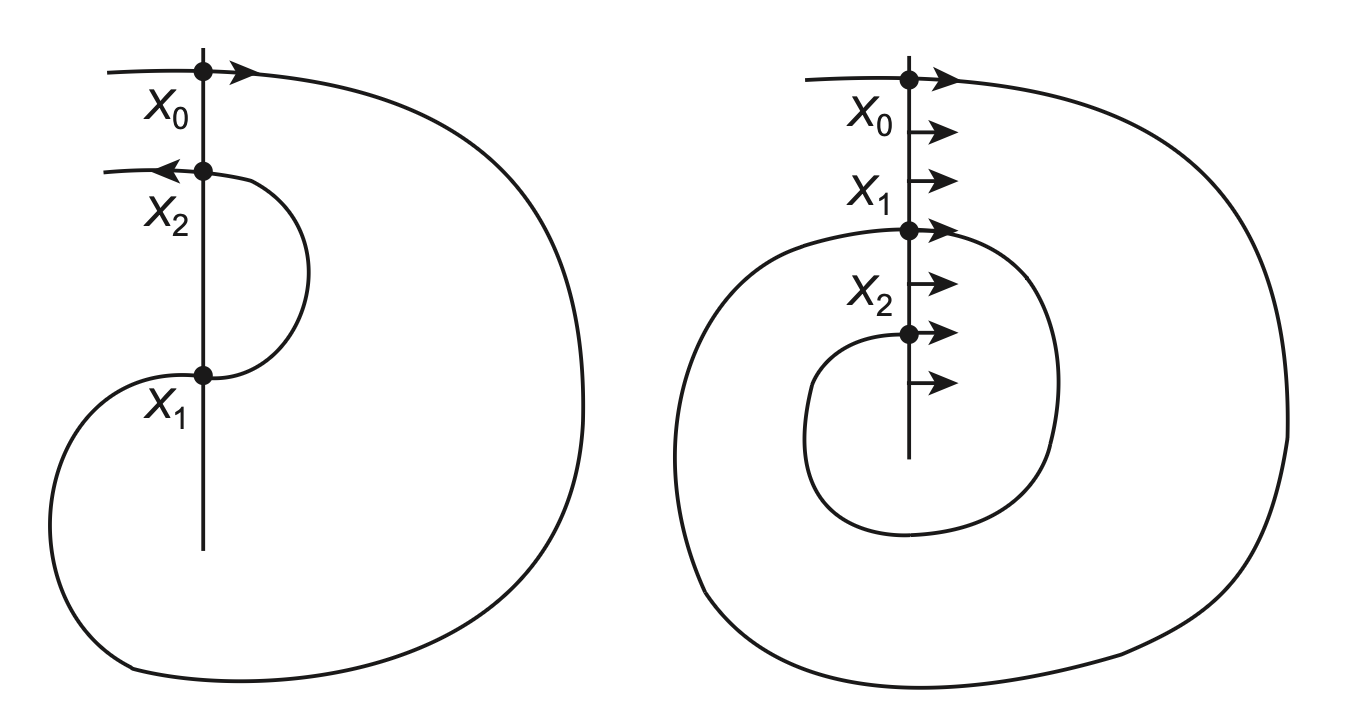
\includegraphics[width=0.4\textwidth]{12-4-1.png}
		\captionof{figure}{Two solutions crossing a straight line. On the left, $X_0,X_1,X_2$ is monotone along the solution but not along the line. We expect the vector field of  $F$ to yield the picture on the right when taking the line as a local section.}
	\end{center}
}If a sequence of points is on the intersection of a solution curve and a segment $I$, they may be monotone along the solution curve but not monotone along the segment, or vise versa. However, if $I$ is a local section in the plane, then this is not possible.


\begin{prop}
	Consider the local section $S_{X_0}$ and suppose $Y_i = \phi_{t_i}(X) \in S_{X_0}$ for $t_1 < t_2 < \ldots$.
	Then $Y_1,Y_2,\ldots$ are monotone along $S_{X_0}$, i.e. $Y_n$ is between $Y_{n-1}$ and $Y_{n+1}$.
\end{prop}

\begin{proof}
	It suffices to prove that any three points $Y_0,Y_1,Y_2$ are monotone.\marginnote{This is because once we have that $Y_0,Y_1,Y_2$ are monotone, we know that $Y_2,Y_3,Y_4$ must be monotone and so on.}
	\marginnote{
		\begin{center}
			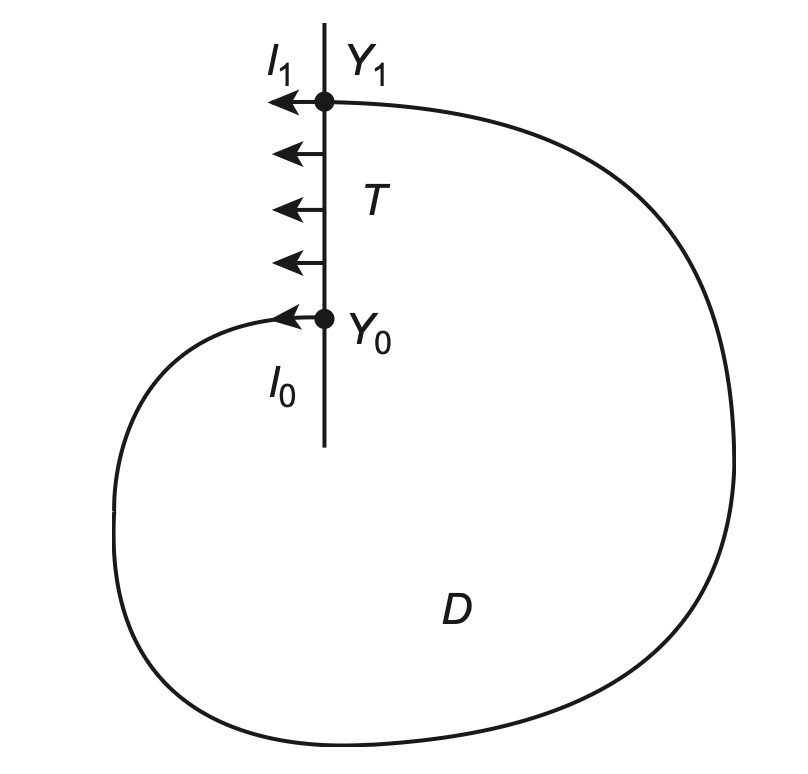
\includegraphics[width=0.4\textwidth]{12-4-2}
			\captionof{figure}{Solutions exit $D$ through $T$.}
		\end{center}
	}

	Define $\Sigma$ as the trajectory between $Y_0$ and $Y_1$, i.e. \[
		\Sigma = \{\phi_t(X) : t \in [t_0,t_1]\}
	.\] 
	Now define $T$ be the segment of $S_{X_0}$ between $Y_0$ and $Y_1$. We can set a region $D$ as a domain with boundary $\Sigma \cup T$. It has an interior and exterior.

	Assume that $\phi_t(x)$ leaves the closure of $D$ at $Y_1$.\footnote{We can also have $F(Y_1)$ entering $D$. This leads to $D$ being positive invariant.} Then $D^{c}$ is positive invariant, because any trajectory starting from $D^{c}$ cannot enter $D$ unless it crosses $\Sigma$, which violates uniqueness of the solution. Furthermore, trajectories cannot enter through $T$ due to the direction of the flow there. More specifically, \[
		\forall\ z \in D^{c}, \qquad \phi_t(z) \not\in \Sigma, \phi_t(z) \not\in T
	.\] 

	By our assumption of $\phi_t(x)$ leaving the closure of $D$ at $Y_1$, we have that for any $\epsilon > 0$, $\phi_{\epsilon}(Y_1) \in D^{c}$. Furthermore, since we cannot reenter $D$, we have that \[
		Y_2 = \phi_{t_2-t_1}(Y_1) \in D^{c}
	.\] 

	We can decompose $S = T \cup I_0 \cup I_1$ as in the diagram, where $I_0$ and $I_1$ each have one of their endpoints at $Y_0$ and $Y_1$. Formally, we define $T$ to be the line segment of $S$ with endpoints $Y_0$ and $Y_1$
	define
	\[
	  I_0, I_1
	\]
	to be the two connected components of $S_{X_0}\setminus T$, labelled so that
	\[
	  Y_0 \in \overline{I_0}, \qquad
	  Y_1 \in \overline{I_1},
	\]
	where the closures are taken inside $S$.
	into three disjoint segments.
	
	We know $Y_2 \in S$ and $Y_2 \not\in T$. We want to show that $Y_2 \in I_1$, but first have to show that $I_1 \subseteq D^{c}$ and $I_0 \subseteq D$. This is not trivial. If we can show this, then since $Y_2 \in I_0$ or $I_1$ and $Y_2 \in I_1 \subseteq D^{c}$, we know
	\begin{align*}
		Y_2 &\in D^{c} \cap \left( I_1 \cup I_0 \right)  = D^{c} \cap I_1\\
		\implies Y_2 &\in I_1 \implies \text{ monotone}
	.\end{align*}

	Suppose for contradiction that $I_1$ contains a point of $D$, so there exists $p \in I_1 \cap D$.
	By shrinking the neighborhood of $Y_1$ along $S$ if necessary, we may assume
	that $p$ is arbitrarily close to $Y_1$.
	Then \[
		[\phi_\epsilon(Y_1), p] \cap \Sigma = \phi_{-\beta}(Y_1)
	\] for some $\beta > 0$.\marginnote{We know that the point where the segment crosses $\Sigma$ will be backwards in time from $Y_1$ because $\Sigma$ is defined as the trajectory between $Y_0$ and $Y_1$.} This is because one end of the line segment is in $D^{c}$, while the other end is in $D$. Because $D$ is open, the segment must cross the boundary; we guarantee it crossing $\Sigma$ by requiring $p$ to be close to $Y_1$. 

	We can write
	\begin{align*}
		\phi_{-\beta}(Y_1) &= \lambda_\beta \phi_\epsilon(Y_1) + (1-\lambda \beta) p \\
		\left[ \phi_{-\beta}(Y_1) - Y_1 \right] &= \lambda_\beta \left[ \phi_\epsilon(Y_1) - Y_1 \right] + (1-\lambda_\beta)(p - Y_1)
	.\end{align*}
	Taking the dot product of each term with $F(Y_1)$, we see that we have the left hand side is negative, the first on the right hand side is positive and the second is zero, an impossiblity.

	Hence $I_1 \in D^{c}$ and $I_2 \in I_1$.
\end{proof}

\marginnote{
	\begin{center}
		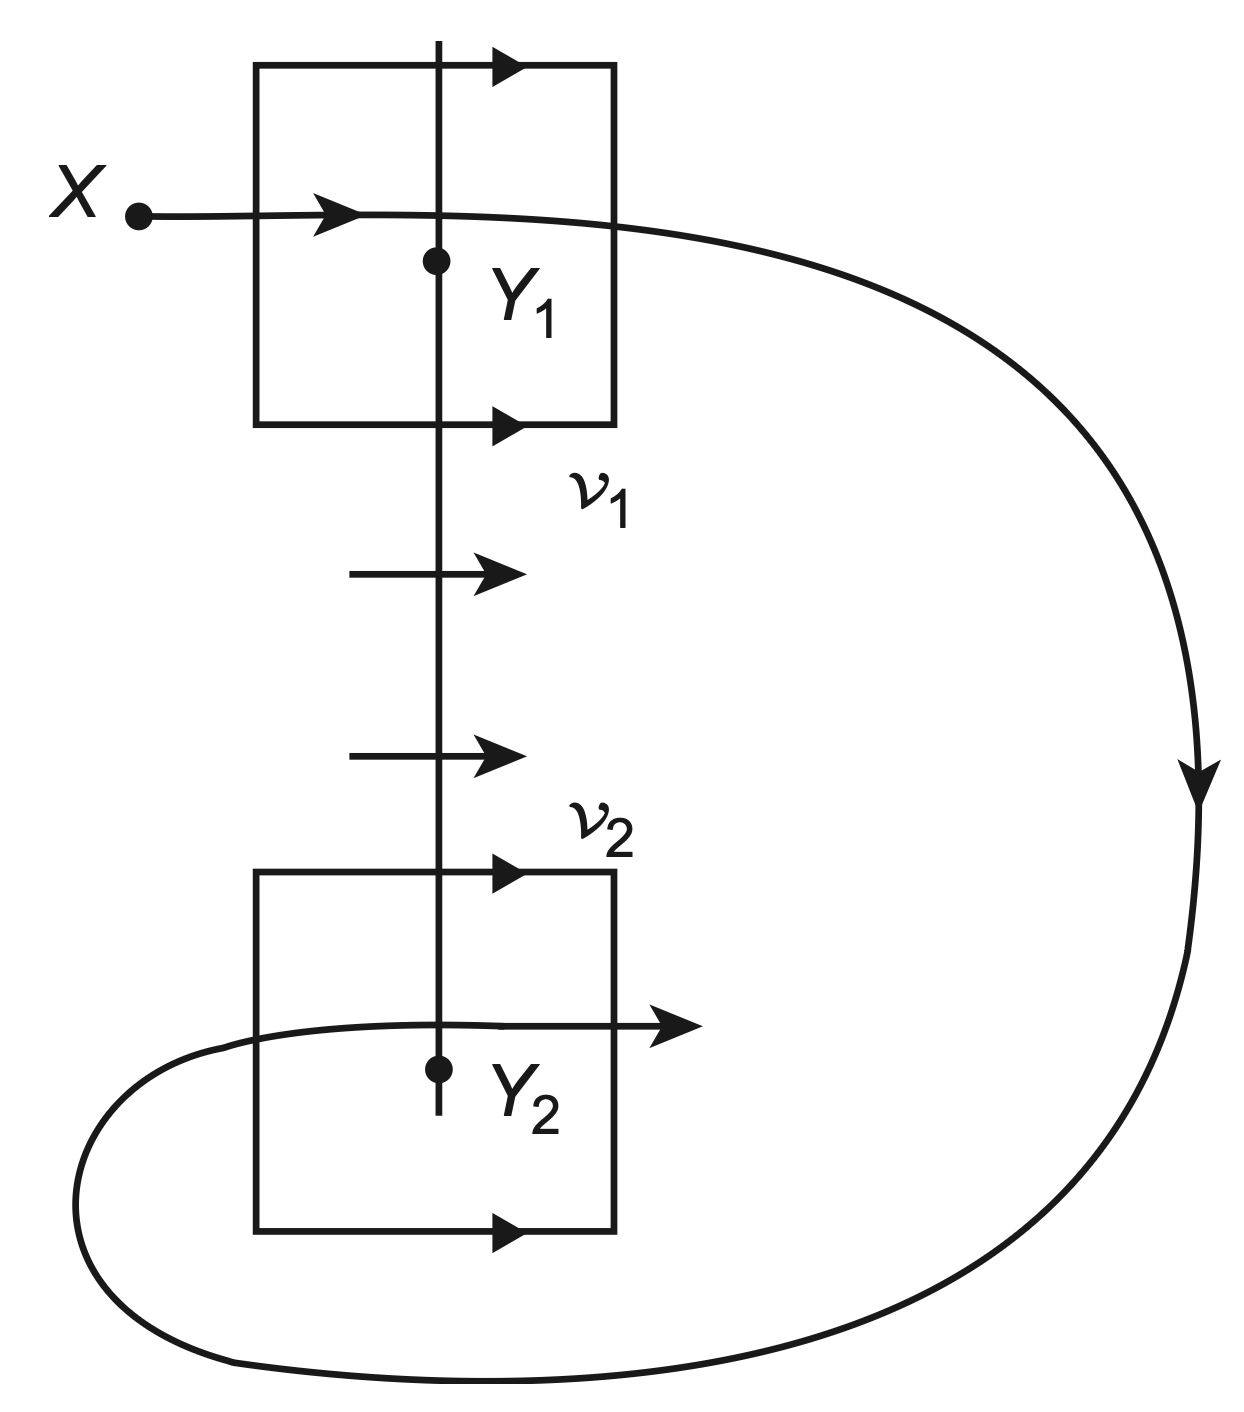
\includegraphics[width=0.4\textwidth]{12-4-3}
	\end{center}
}
\begin{cor}
	Suppose $Y \in \omega(X)$. Let $Z$ be any point with $F(Z)\ne 0$ and let $S$ be a local section at $Z$. Then the solution through $Y$ crosses any local section $S$ at most $1$ point.Equivalently, if $\phi_{t_1}(Y)\in S$ and $\phi_{t_2}(Y)\in S$,
then $\phi_{t_1}(Y)=\phi_{t_2}(Y)$.
\end{cor}

\begin{proof}
	Fix $Y \in \omega(X)$ and a local section $S$. Suppose for contradiction that there exist $Y_1,Y_2 \in S$ such that \[
		Y_i = \phi_{t_i}(Y)
	.\] We can draw flow boxes of size $\sigma$ around $Y_1$ and $Y_2$ that do not intersect, i.e. there exist $\nu_{1,\sigma} \cap \nu_{2,\sigma} = \O$. The flows point in the same direction because both boxes contain part of the local section.

	We know that the limiting set $\omega(X)$ is an invariant set. Hence, $Y_1, Y_2 \in \omega(X)$. Therefore we have sequences \[
		\phi_{t_n}(x) \to Y_1, \quad \phi_{s_n}(x) \to Y_2
	,\] where $\phi_{t_n}(x) \in \nu_{1,\sigma}$ and $\phi_{2, \sigma}$.

	We can adjust the times slightly to land on the local section: \[
		\phi_{t_n + o(\sigma)}(x) \in S, \quad \phi_{s_n + o(\sigma)}(x) \in S
	.\] 
	Then \[
		t_{1+o(\sigma)} < s_{k + o(\sigma)} < t_{n + o(\sigma)}
	\] by definition of $Y_1$ and $Y_2$. Label the corresponding points of $\phi_t(X)$ as $A,B,$ and $C$, so by the previous proposition, we know that $A,B,C$ are monotone along the local section. $A$ and $C$ are in the first box, while $B$ is in the second box, which is disjoint from the first. This is a contradiction.
\end{proof}

\begin{thm}
	(Poincar\'e-Bendixson) 
	Suppose $\omega(X) \ne \O$ and is topologically closed and bounded. If $\omega(X)$ does not contain an equilibrium, then $\omega(X)$ is a closed orbit.
\end{thm}
\marginnote{If we have $\{\phi_t(x)\} \subseteq D$ for all $t \ge 0$, then $\omega(X) \ne \O$.}

\begin{proof}
	We know that $\omega(X)$ is an invariant set. Fix $Y \in \omega(X)$, so $\phi_t(Y) \in \omega(X)$ for every $t \ge 0$, i.e. $\omega(Y) \subseteq \omega(X)$. Since $\omega(X)$ is bounded, any subsequence $\phi_{t_n}(Y)$ will have a convergent subsequence, so $\omega(Y)$ is nonempty.

	Fix $Z \in \omega(Y) \subseteq \omega(X)$. Since $\omega(X)$ does not contain an equilibrium, $F(Z) \ne 0$.

	We then have a local section $S_Z$ of $Z$. Putting a flow box $\nu_\sigma$ around $Z$ and $Z \in \omega(Y)$ implies that we have some sequence $\{t_n\}$ where $\phi_{t_n} (Y) \to Z$, we know that for some $N \in \N$, $n \ge N$ implies \[
		\phi_{t_n} (Y) \in \nu_\sigma
	.\] We can adjust the time a bit to get \[
		\phi_{t_n + o(\sigma)}(Y) \in S_Z
	\] for all $n \ge N$. By the previous corollary, this implies that these times must all correspond to the same point: \[
		\phi_{t_N + o(\sigma)}(Y) = \phi_{t_{N+1} + o(\sigma)} = \ldots
	.\] Putting $\tau = \min \left\{ t_N + o(\sigma), t_{N+1} + o(\sigma), \ldots \right\}$\marginnote{should be $\inf$ but then is it still periodic?)}, we see \[
		\phi_\tau(Y) = Y
	,\] meaning $\phi$ started from $Y$ is periodic. Let $\gamma$ be the closed orbit through $Y$, so because $Y \in \omega(X)$, $\gamma \subseteq \omega(X)$.

	We claim that $\gamma = \omega(X)$ and \[
		\lim\limits_{t \to \infty} \operatorname{dist}\left( \gamma, \phi_t(x) \right) = 0
	.\] Fix $Y \in \omega(X)$, so $F(Y) \ne 0$. We get that there is some sequence $\tau_1 < \tau_2< \ldots$ such that \[
		\phi_{t_n}(X) \to Y, \quad \phi_{t_n}(X) \in S_Y
	,\] and for any $t \in (t_n, t_{n+1})$, \[
		\phi_t(X) \not\in S_Y
	.\] Pick $0 < \epsilon < \tau$. By continuous dependence, \[
		\left| \phi_s(Y) - \phi_{s + t_n} \right| \le c_\tau \left| Y - \phi_{t_n}(X) \right|
	\] for any $0 \le s \le 2t$ and $n \ge 1$.

	Taking $n$ large, since $\phi_\tau(Y) = Y$, we pick $s = \tau$ to get \[
		\left| \phi_{\tau + t_n}(X) - Y \right| < \epsilon
	.\] Furthermore, \[
		\left| t_{n+1} - \tau - t_n \right| < \epsilon > \tau
		.\] Note that $\phi_s(Y) \in \gamma$, so by the continuous dependence result and taking $0 \le s \le t_{n+1} - t_n  <2\tau$
, \[
		\operatorname{dist}\left( \gamma, \phi_{\left[ t_n, t_{n+1} \right]} \right) \le C_\tau \left| Y - \phi_{t_n}(X) \right|
	.\] Sending $n \to \infty$ yields \[
		\operatorname{dist}\left( \gamma, Y \right) = 0
	.\] 
\end{proof}

\begin{cor}
	Suppose that $K$ is a closed, bounded, and positive (negative) invariant set. Then $K$ contains an equilibrium or a closed orbit.	
\end{cor}

\begin{proof}
	Pick $X \in K$.
	Since $K$ is positive invariant and closed, we have \[
		\omega(X) \subseteq K, \qquad \phi_t(X) \in K, \forall\ t \ge 0
	.\] 
	$K$ is bounded, so any sequence $t_n$ has a subsequence $t_{n_k}$ where $\phi_{t_{n_k}}$ is convergence. Because $K$ is closed, the limit is in $K$, so $\omega(X) \ne \O$.

	If $\omega(X)$ has an equilibrium, we are done. If it does not, we use the Poincar\'e-Bendixon theorem to see that $\omega(X)$ contains a closed orbit $\gamma$.
\end{proof}
	
\begin{ex}
	Consider \[
		\frac{d}{dt}X = F(X)
	,\] where \[
		X \cdot F(X) \left.\right|_{\partial B_R}
	\] for a positive invariant $B_R$. If \[
		n \cdot F(X) \left.\right|_{\partial D} < 0
	,\] then $D$ is positive invariant. \texthl{???}\marginnote{The first example is from the book and the second example is supposed to say that if $X\cdot F(X) > 0$ on the boundary of some region, then that region is positive invariant.}
\end{ex}



\section{Textbook Notes}

\subsection{Teschl -- 2.4: Dependence on the Initial Condition}
\begin{thm}
	(Gronwall's inequality) Suppose $\psi(t)$ satisfies \[
		\psi(t) \le \alpha(t) + \int_{0}^{t} \beta(s)\psi(s)ds ,\quad t \in [0,T]
	\] for $\beta \ge 0$. Then \[
	\psi(t) \le \alpha(t) + \int_{0}^{t} \alpha (s) \beta(s) \operatorname{exp}\left(\int_{s}^{t} \beta(r)dr \right)ds , \quad t \in[0,T]
	.\] We can IBP to find also that
	\begin{align*}
		\psi(t) &\le \alpha(0) \operatorname{exp}\left(\int_{0}^{t} \beta(r)dr \right) + \int_{0}^{t} \alpha'(s) \operatorname{exp}\left(\int_{s}^{t} \beta(r)dr \right)ds  
	.\end{align*}
\end{thm}

\begin{proof}
	Write $B(t) = \operatorname{exp}\left(-\int_{0}^{t} \beta(s)ds \right)$. Then
	\begin{align*}
		\frac{d}{dt}B(t) \int_{0}^{t} \beta(s)\psi(s)ds &= B(t)\cdot \left( -\beta(t) \right) \int_{0}^{t} \beta(s)\psi(s)ds + B(t) \beta(t)\psi(t) \\
													 &= \left(B(t) \beta(t) \right) \left( \psi(t) - \int_{0}^{t} \beta(s)\psi(s)ds  \right) \\
													 &\le B(t)\beta(t) \alpha(t)
	,\end{align*}
	where the last line follows from the theorem assumption. Integrating (an operation that preserves the inequality, unlike differentiation), we get 
	\begin{align*}
		B(t) \int_{0}^{t} \beta(s)\psi(s)ds - B(0) \int_{0}^{0} \beta(s)\psi(s)  &\le \int_{0}^{t} B(s) \beta(s)\alpha(s) ds \\  
		\int_{0}^{t} \beta(s) \psi(s)ds &\le \int_{0}^{t} \frac{B(s)}{B(t)} \beta(s) \alpha(s)ds \\
		\psi(t) \le \alpha(t) + \int_{0}^{t} \beta(s) \psi(s)ds &\le \alpha(t) + \int_{0}^{t} \alpha(s)\beta(s) \frac{B(s)}{B(t)}ds \\
																&= \alpha(t) + \int_{0}^{t} \alpha(s)\beta(s) \operatorname{exp}\left( -\int_{0}^{s} \beta(r)dr + \int_{0}^{t} \beta(r)dr  \right) \\
																&= \alpha(t) + \int_{0}^{t} \alpha(s)\beta(s) \operatorname{exp}\left(\int_{s}^{t} \beta(r)dr \right) 
	.\end{align*}
\end{proof}

\begin{thm}
	(Continuous dependence on initial conditions and parameters) Suppose $f$ is Lipschitz in its second argument with constant $L$\marginnote{$f$ just needs to be Lipschitz on a set $V$ in $\R^{1 + n}$ that contains the graphs of $x(t)$ and $y(t)$} and continuous in its first. For a given function $g$, if $x(t)$ and $y(t)$ are respective solutions of
	\begin{align*}
		\frac{d}{dt} x &= f(t,x), \quad x(t_0) = x_0 \\
		\frac{d}{dt}y &= g(t,y), \quad y(t_0) = y_0
	,\end{align*}
	then \[
		\left| x(t) - y(t) \right| \le \left| x_0-y_0 \right|e^{L \left| t-t_0 \right|} + \frac{M}{L} \left( e^{L \left| t-t_0\right|} - 1 \right)
	,\] where \[
		M := \sup_{(t,x) \in V} \left| f(t,x) - g(t,x) \right|
	.\]  
\end{thm}

\begin{proof}
	We have that
	\begin{equation}
		 \label{eq:contdep}
		\left| x(t) - y(t) \right| \le \left| x_0-y_0 \right|  + \int_{t_0}^{t} \left| f(s,x(s)) - g(s,y(s))  \right|ds 
	.\end{equation}
	
	We get that
	\begin{align*}
		\left| f(s,x(s)) - g(s,y(s)) \right| &\le \left| f(s,x(s)) - f(s,y(s)) \right| + \left| f(s,y(s) - g(s,y(s)) \right| \\
											 &\le L \left| x(s) - y(s) \right| + M
	.\end{align*}
	Plugging this back into (\ref{eq:contdep}), we get
	\begin{align*}
		\left| x(t) - y(t) \right| &\le \left| x_0-y_0 \right| + \int_{t_0}^{t} L \left| x(s) - y(s) \right| + M ds \\
		&= \left| x_0-y_0 \right| + Mt + \int_{t_0}^{t} L \left| x(s) - y(s) \right| ds
	.\end{align*}
	We can use Gronwall's inequality (IBP form) with \[
		\alpha(t) = \left| x_0-y_0 \right| + Mt, \quad \beta(t) = L
	\] to get that \[
		\left| x(t) - y(t) \right| \le \left| x_0-y_0 \right| \operatorname{exp}\left(\int_{t_0}^{t} L dr \right) + \int_{t_0}^{t} M \operatorname{exp}\left(\int_{s}^{t} Ldr \right)ds
	,\] so
	\begin{align*}
		\left| x(t) - y(t) \right|&\le \left| x_0-y_0 \right|e^{Lt} + M \int_{t_0}^{t} e^{L(t-s)}ds \\ 
								  &= \left| x_0-y_0 \right|e^{Lt} + \frac{M}{L} \left(e^{L(t - t_0)}-1\right)
	.\end{align*}
\end{proof}

\subsection{Comparison}

\begin{thm}
	(Comparison) Suppose $F$ is Lipschitz in its second argument and $f,g$ are differentiable. If
	\begin{align}
		f' &\le F(t,f(t)), \forall\ t \in [a,b] \label{comp1}\\
		g \text{ solves } g' &= F(t,g(t)) \label{comp2} \\
		f(a) &\le g(a), \label{comp3}
	\end{align}
	then \[
		f(t) \le g(t), \quad \forall\ t \in [a,b]
	.\]
\end{thm}

\begin{proof}
	Suppose for contradiction that there exists $t_1 \in [a,b]$ such that $f(t_1) > g(t_1)$. We assume WLOG (just shrink $b$) that for $t > t_1$, $f(t) > g(t)$ still. Define \[
		\Omega = \{t: f(t) \le g(t)\}
	.\] $\Omega$ is nonempty because it includes $a$, so we can put \[
		t_0 := \sup \{t \in \Omega \cap [a,t_1]\}
	.\] By definition, we have that for all $t \in [a,t_0)$, $f(t) \le g(t)$, and for $t \in (t_0, t_1]$, $f(t) > g(t)$. By continuity from the left and right sides, $f(t_0) = g(t_0)$. 

	By assumption, $F$ is Lipschitz in its second argument on $[a,b]$ by constant $L$. Note that by (\ref{comp1}) and (\ref{comp2}), we have that for every $t$,
	\begin{align*}
		\left| f'(t) - g'(t) \right| &\le F(t,f(t)) - F(t,g(t)) \\
		f(t) - g(t) &\le \left| f(t_0) - g(t_0) \right| + \int_{t_0}^{t} F(s,f(s)) - F(s,g(s)) ds  \\
					&\le 0 + \int_{t_0}^{t} L \left| f(s)-g(s) \right|ds
	.\end{align*}
	In particular, for $t \in [t_0, t_1]$, the interval on which $f \ge g$, we have \[
		f(t) -g(t) \le \int_{t_0}^{t} L \left( f(s) - g(s) \right)ds 
	.\] We apply Gronwall's inequality (IBP form) to this with $\alpha = 0$ and $\beta = L$ to see \[
		f(t) -g(t) \le 0
	\] for $t \in [t_0,t_1]$, a contradiction.

\end{proof}

\subsection{Teschl -- 2.6: Extensibility of Solutions}
\begin{lemma}
	(Gluing lemma) Suppose $f(t,x(t))$ is continuous and Lipschitz in any bounded region. Suppose $\phi_i(t)$ solves \[
		\frac{d}{dt}\phi_i(t) = f(t,\phi_i(t))
	\] for $t \in I_i=(a_i,b_i)$. If $t_0 \in I_1 \cap I_2$ and $\phi_1(t_0) = \phi_2(t_0)$, then the solutions agree on $I_1 \cap I_2$ and can be glued together on $I_1 \cup I_2$: \[
		\phi_1(t) = \phi_2(t), \quad t \in I_1\cap I_2
	,\] \[
		\phi(t) = \begin{cases}
			\phi_1(t), \quad t \in I_1 \\
			\phi_2(t), \quad t \in I_2
		\end{cases}
	\] is a $C^1$ solution to \[
		\frac{d}{dt} x(t) = f(t,x(t))
	\] on $I_1 \cup I_2$.

\end{lemma}

\begin{proof}
	\newthought{(Proof 1)} 
	Let $I = I_1 \cap I_2 = (T_-, T_+)$ and let $(t_-,t_+)$ be defined \[
		t_- = \inf \{t \in I : \phi_1(t) = \phi_2(t)\}, \quad t_+ = \sup \{t \in I : \phi_1(t) = \phi_2(t)\}
	.\]  We claim that $t_+ = T_+$. Suppose towards a contradiction that $t_+ < T_+$ (this is sufficient, since $t_+ > T_+$ is not possible by definition of the maximal interval).

	For every $t \in (t_-, t_+)$, $\phi_1(t) = \phi_2(t)$. $\phi_1$ and $\phi_2$ are defined at $t_+$ because $t_+ < T_+$, so $t_+ \in I$. By continuity, we see that $\phi_1(t_+) = \phi_2(t_+)$. Since $F$ was assumed to be continuous and Lipschitz in its second argument on a bounded region\footnote{Say, a rectangle containing the graph of $\phi_1$ and $\phi_2$ on $[t_+ - \delta, t_+ + \delta]$}, it satisfies the conditions for the existence-uniqueness theorem. The initial conditions and differential equations for $\phi_1$ and $\phi_2$ coincide, so they must coincide in a neighborhood of $t_+$ by local existence and uniqueness, contradicting maximality of $t_+$. So, $t_+ = T_+$. Similarly, $t_- = T_-$.

	This implies that the function \[
		\phi(t) = \begin{cases}
			\phi_1(t), \quad t \in I_1 \\
			\phi_2(t), \quad t \in I_2
		\end{cases}
	\] is well-defined. Since it is $C^1$ on $I_1$ by looking at $\phi_1$ and $C^1$ on $I_2$ by looking at $\phi_2$, it is $C_1$ on $I_1 \cup I_2$. It is a solution to the ODE on $I_1 \cup I_2$.

	\newthought{(Proof 2)} 
	Define $I = I_1 \cap I_2$ and fix $\left[ \alpha,\beta \right] \in I$ as a compact interval that contains $t_0$. By $F$ being locally Lipschitz, there exists $L \ge 0$ such that 
	\begin{align*}
		\phi_1(t) - \phi_2(t) &= \int_{t_0}^{t} F(s,\phi_1(s)) - F(s, \phi_2(s)) ds \\
							  &\le L \int_{t_0}^{t} \left| \phi_1(s) - \phi_2(s) \right|ds \\
							  &\le L \int_{\alpha}^{\beta} \left| \phi_1(s) - \phi_2(s) \right|ds 
	.\end{align*}
	Applying post-IBP Gronwall (so $\alpha(0) = 0, \alpha' = 0$), \[
		\phi_1(t) - \phi_2(t) \le 0
	\] for all $t \in [\alpha,\beta]$. Since $\alpha, \beta$ were arbitrary, $\phi_1(t) = \phi_2(t)$ for all $t \in I$. We can glue and get that $\phi$ is $C^1$ from it being $C^1$ on $I_1$ and $I_2$.

	\newthought{(Proof 3)} 
	Define $I = I_1 \cap I_2$. Define \[
		S = \{t \in I : \phi_1(t) = \phi_2(t)\}
	.\] Because $\phi_1 - \phi_2$ is continuous, for any convergence sequence $\{t_n\} \to t^*$ in $S$, \[
		\left( \phi_1-\phi_2 \right)(t) = (\phi_1-\phi_2) (\lim\limits_{n \to \infty} t_n) = \lim\limits_{n \to \infty} 0 = 0
	,\] so $S$ is closed in $I$.

	Fixing $t \in S$, by existence-uniqueness, since $\phi_1(t) = \phi_2(t)$, they must be defined and agree on a neighborhood of $t$, so $S$ is open in $I$.

	$I$ is a connected interval and is nonempty (it contains $t_0$), so $S=I$.
\end{proof}

\begin{thm}
	(Blowup Criterion) Let $\phi(t)$ be a solution to $\frac{d}{dt}x = f(t,x)$ on the interval $(t_-, t_+)$ given some specific initial condition. Then there exists an extension to the interval $(t_-, t_+ + \epsilon)$ for some $\epsilon > 0$ iff there exists a sequence $\{t_n\} \in (t_-, t_+)$ such that \[
		\lim\limits_{n \to \infty} \left( t_n, \phi(t_n) \right) = (t_+, y)
	\] for some $y \in \R$. In other words, the solution can be extended iff the graph $(t_n, \phi(t_n))$ has a finite limit point.
\end{thm}

\begin{proof}
	($\implies$) Pick any sequence $t_n \uparrow t_+$. By continuity of $\phi$, we see that there must be a limit point, which is just $(t_+, \phi(t_+)$.

	($\impliedby$) Suppose we have a sequence with a finite limit point, so we have a sequence $\{t_n\} \in (t_-, t_+)$ such that $\lim\limits_{n \to \infty} (t_n, \phi(t_n)) = (t_+, y)$.

	There exists some $N$ such that for all $n \ge N$, $\left| \phi(t_n) - y \right| \le 1$ and $\left| t_n - t_+ \right| \le 1$. On this square \[
		S:= \left[ t_+ - 1, t_+ +1 \right]\times \left[ y-1,y+1 \right]
	,\] we have that $f$ is continuous and Lipschitz with uniform bound $L$. These give the bounds \[
		\begin{cases}
			\phi'(t_n) = \left| f(t_n, \phi(t_n)) \right| < M \\
			\left| f(t, x) - f(t, z) \right|\le L \left| x-z \right|
		\end{cases}
	.\] Recall that in the existence-uniqueness proof, we required \[
		h < \min \{\frac{1}{L}, \frac{b}{M} = \frac{1}{M}, a = 1\}
	.\] In particular, this is not dependent on which particular $t_n$ we want to solve the ODE in a neighborhood on, so we can fix $h > 0$ for which the solution to the ODE exists on every $B_h(t_n)$ for all $n \ge N$.

	Since $t_n \uparrow t_+$, there exists $t_M$ such that $\left| t_+ - t_M \right| < h$, so $t_M + h > t_+$. Then by the existence-uniqueness theorem, we can solve the ODE on an interval including $t_+$. By the gluing lemma, we have a $C^1$ solution defined on $(t_-, t_+ + \epsilon)$ for some $\epsilon > 0 $.

\end{proof}

\begin{cor}
	We see that the solution cannot be extended iff \[
		\lim_{t_n \to \infty} f(t,\phi(t_n)) = \infty
	\] for every sequence $t_n \uparrow t_{+}$.

	By definition of $\liminf$, the solution can be extended iff \[
		\left|  \liminf_{t \to t_+} f(t,\phi(t))\right| < \infty
	.\] 
\end{cor}

\subsection{Boyce, DiPrima, Meade -- 9.2 Autonomous Systems and Stability}

Consider \[
	\frac{d}{dt}x = f(x,y),\ x(t_0) = x_0, \quad \frac{d}{dt}y = g(x,y),\ y(t_0) = y_0
,\] whihc we write as \[
	\frac{d}{dt}x = F(x), \quad x(t_0) = x_0
\] for $x: \R \to \R^2$ and $F: \R^2 \to \R^2$.

This system is called autonomous because $f$ and $g$ do not depend on the independent variable $t$ but instead only on the dependent variables $x$ and $y$.

Autonomous systems are interesting because they have an associated vector field that is independent of time. Consequently, there is only one trajectory passing through each point in the phase plane. All solutions that satisfy a given initial condition must lie on the same trajectory, regardless of the time at which they pass through the initial condition's point.

The following definitions are in the context of the autonomous system \[
	\frac{d}{dt}x = F(x), \quad x(t_0) = x_0
.\] 

\begin{defn}[Critical point]
	A point $x$ is called a critical point of the autonomous system if $f(x) = 0$. These are also called constant or equilibrium solutions of the system of differential equations.
\end{defn}

\begin{defn}[Stable, unstable]
	A\marginnote{Under the assumption that $F$ is locally Lipschitz, the solution cannot blow up, so we are guaranteed existence for all $t \ge t_0$.} critical point $x^*$ is stable if for any $\epsilon > 0$, there exists $\delta> 0$ such that every solution $x=x(t)$ that satisfies \[
		\|x(t_0) - x^*\| < \delta
	\] satisfies \[
		\|x(t) - x^*\| < \epsilon
	\] for all $t \ge t_0$.

	A critical point is unstable if it is not stable.
\end{defn}

\begin{defn}[Asymptotically stable]
	A critical point is asymptotically stable if 
	\marginnote{The precondition of stability is needed to exclude families of trajectories that have members who start arbitrarily close to $x^*$ then depart an arbitrarily large distance before eventually tending to $x^*$.}
	\begin{enumerate}[(i)]
		\item it is stable, and 
		\item there exists $\delta > 0$ such that if $\|x(t_0) - x^*\| \le \delta$, then \[
			\lim\limits_{t \to \infty} x(t) = x^*
		.\] 
	\end{enumerate}
\end{defn}

\subsection{Boyce, DiPrima, Meade -- Locally Linear Systems}

Consider \[
	\frac{d}{dt}x = Ax
\] for a constant matrix $A \in \R^n\times \R^n$.
\begin{thm}
	(Linear stability of steady state) A critical point $x^*$ of the system is
	\begin{enumerate}[(i)]
		\item asymptotically stable if all eigenvalues of $A$ have negative real part;
		\item stable and not asymptotically stable if all eigenvalues are purely imaginary; and 
		\item unstable if at least one eigenvalue of $A$ has positive real part.
	\end{enumerate}
\end{thm}




\subsection{Braun -- 4.3: Stability of Equilibrium Solutions}

Consider the equation \[
	\frac{d}{dt}X = AX + g(X), \quad X \in \R^n
.\] Assume $g$ is satisfies $\lim\limits_{x \to 0} \frac{\|g(x)\|}{\|x\|} = 0$ and the quotient is continuous, i.e. $\frac{d}{dt}X$ is $C^1$. We see that since $g(0) = 0$, $X(t) = 0$ is an equilibrium solution of the ODE. We want to determine the stability of this equilibrium at the origin.

\begin{aside}
	We recall some real analysis facts. Suppose $\frac{d}{dt}X = F(X)$ and $F$ is differentiable. We can Taylor approximate around some point $X_0$ with \[
		\frac{d}{dt}X = F(X_0) + \nabla F(X_0) + (X- X_0) + G(X-X_0)
	\] for some function $G$ such that \[
		\lim\limits_{X \to X_0} \frac{\left\| G(X - X_0) \right\|}{\left\| X-X_0 \right\|} = 0
	.\] Similarly, if $F \in C^2$, then $G$ satisfies \[
		\lim\limits_{X  \to X_0} \frac{\left\| G(X-X_0) \right\|}{\|X-X_0\|^2} = 0
	.\] We say that $G(X-X_0) = o\left( \left( X-X_0 \right) \right)$ and $G(X-X_0) = o\left( \left( X-X_0 \right)^2 \right)$ respectively. 

	$g$ is big-O of $\|X-X_0\|^{k}$ at $X_0$ if there exist $C \in R$ and $\delta > 0$ such that \[
		g(X-X_0) \le C \|X-X_0\|^{k}
	\] for all $\|X-X_0\| < \delta$. We see that by taking $\epsilon = 1$ in the limit definition so eventually $\frac{\|G(h)\|}{\|h\|^{k}} < 1$, we can multiply by $\|h\|^{k}$ to show \[
		g(h) = o(h^{k}) \implies g(h) = O(h^{k})
	.\] However, the converse is not true; consider $g(h) = \left| h \right|$.
\end{aside}

\begin{thm}
	Suppose \[
		\frac{d}{dt}x = Ax + g(x), x \in \R^n
	,\] where $g \in C^2$ and $A$ has eigenvalues $\lambda_1,\ldots,\lambda_n$. Let $x^*$ be an equilibrium, so $Ax^* + g(x^*)$
	\begin{enumerate}[(i)]
		\item The equilibrium solution $x(t) = 0$ is asymptotically stable if $\lambda_1,\ldots,\lambda_n$ all have negative real parts.
		\item The equilibrium solution $x(t) = 0$ is unstable if $\operatorname{Re}\left(\lambda_i\right) > 0$ for at least one $i$.
		\item The stability of $x(t) = 0$ cannot be determined if all eigenvalues have nonpositive real part but at least one eigenvalue has zero real part.
	\end{enumerate}
\end{thm}

\begin{proof}
	\newthought{(Asymptotic stability.)} Suppose that $\operatorname{Re}\left(\lambda_1\right),\ldots,\operatorname{Re}\left(\lambda_n\right) < 0$. By the Duhamel formula for nonlinear first order systems, we can write a solution $x(t)$ of the nonlinear ODE as \[
		x(t) = e^{At}x(0) + \int_{0}^{t} e^{A(t-s)}g(x(s))ds 
	.\] To show asymptotic stability at the origin, we want to show that $\|x(t)\|\to 0$ as $t\to \infty$ for some $x(0)$ close to the origin.

	Because $A$ has eigenvalues all with negative real part, we can find $K, \alpha > 0$\marginnote{\texthl{See exercise 4.2.17 in Braun}} such that \[
		\|e^{At} x(0)\| \le Ke^{-\alpha t} \left| x(0) \right|, \quad \|e^{A(t-s)g(x(s))}\| \le Ke^{-\alpha(t-s)} \|g(x(s))\|
	.\] Because $\frac{g(x)}{\|x\|}$ vanishes at the origin and is continuous (and hence bounded on closed disks), there exists $\sigma > 0$ such that for any $\left| x \right| \le \sigma$, \[
		\|g(x)\| \le \frac{\alpha}{2K} \|x\|
	.\] Plugging these bounds into the Duhamel formula, we get that
	\begin{align*}
		\|x(t)\| &\le \|e^{At} x(0)\| + \int_{0}^{t} \|e^{A(t-s)}g(x(s))\|ds \\ 
				 &\le Ke^{-\alpha t}\|x(0)\| + \frac{\alpha}{2} \int_{0}^{t} e^{-\alpha(t-s)}\|x(s)\|ds \\
		\implies e^{\alpha t} \|x(t)\| &\le K \|x(0)\| + \frac{\alpha}{2} \int_{0}^{t} e^{\alpha s}\|x(s)\| ds
	\end{align*}
	when $\|x(s)\| \le \sigma$. To simplify, we write $d(t) = e^{\alpha t} \|x(t)\|$ to get \[
		d(t) \le K \|x(0)\| + \frac{\alpha}{2 } \int_{0}^{t} d(s)ds 
		.\] We can apply Gronwall's inequality (IBP form) with $\alpha(t) = K \|x(0)\|$ and $\beta(t) = \frac{\alpha}{2} > 0$ to get \begin{align*}
		d(t) &\le \alpha(0) \operatorname{\exp}\left(\int_{0}^{t} \beta(s)ds\right) + \int_{0}^{t} \alpha'(s) \operatorname{exp}\left(\int_{s}^{t} \beta(r)dr\right) ds  \\
			 &= K \|x\left(0 \right)\|\operatorname{exp}\left(\int_{0}^{t} \frac{\alpha}{2} ds\right) + \int_{0}^{t} 0 \cdot \int_{s}^{t} \operatorname{exp}\left(\frac{\alpha}{2}dr \right)ds  \\
			 &= K\|x(0)\|e^{\frac{\alpha}{2}t} 
	,\end{align*}
	which we can substitute $d(t)$ back out to get \[
		e^{\alpha t} \|x(t)\| \le K \|x(0)\|e^{\frac{\alpha}{2}t}
	,\] which implies \[
		\|x(t)\| \le K \|x(0)\|e^{-\frac{\alpha}{2}t}
	,\] as long as $\|x(s)\| \le \sigma$ for all $0 \le s \le t$. If we require $\|x(0)\| \le \frac{\sigma}{K}$, then this is satisfied, so then we have \[
		\|x(t)\| \le K \|x(0)\|e^{-\frac{\alpha}{2}t} \le K \|x(0)\|
	.\] The second inequality gives us stability (we can contain $x(t)$ in a ball by choosing $x(0)$ to be in a small enough ball), and the first inequality shows the other condition for asymptotic stability ($x(t)$ goes to the origin in the infinite horizon).


\end{proof}

\subsection{Hirsch, Smale, Devaney -- 9: Global Nonlinear Techniques}

Consider \[
	\frac{d}{dt}X = F(X), \quad X = (x_1,\ldots,x_n)
.\]
\begin{defn}[Nullcline]
	The $x_j$-nullcline is the set of points where $x_j' = f_j(x_1,\ldots,x_n) = 0$.
\end{defn}

The nullclines decompose $\R^n$ into a collection of open sets, in each of which the vector field points in a certain direction in relation to the standard basis vectors. These regions are called basic regions. The intersection of all nullclines yield the equilibrium points. 

\begin{defn}[Hyperbolic]
	We say that a matrix $A$ is hyperbolic if none of its eigenvalues has real part $0$.

	Let $F : \R^n \to \R^n$ be $C^1$ and consider the autonomous system
  \[
    Y' = F(Y).
	\]
	An equilibrium point $Y^*$ is called hyperbolic if the Jacobian matrix $J_F(Y^*)$
	is hyperbolic. In this case we also say that the system is hyperbolic at $Y^*$.

	The linearization of $Y' = F(Y)$ at the equilibrium $Y^*$ is the linear system
	\[
	  Z' = A Z, \qquad A := D F(Y^*) = J_F(Y^*),
	\]
	and $Y^*$ is hyperbolic iff this linear system is hyperbolic.

\end{defn}

It's easy to determine the stability of an equilibrium point when it is hyperbolic; we can use the theorem on nonlinear stability, in which case the analysis just depends on the magnitude of the real components of the eigenvalues of the Jacobian/total derivative.

When the equilibrium point is not hyperbolic, we must use Lyapunov's method.

\begin{defn}[Basin of attraction]
	The basin of attraction of an asymptotically stable equilibrium point is the set of all initial conditions with solutions that tend to the equilibrium point.
\end{defn}

\begin{defn}[Lyapunov function]
	Let $O \subseteq \R^n$ be open and $L: O \to R$ be differentiable. Suppose $X^* \in O$, where $X^*$ is an equilibrium of the system \[
		\frac{d}{dt}X = F(X)
	.\]
	A scalar function $L: O \to R$, which we call a Lyapunov candidate, has derivative along the vector field given by \[
		\dot{L}(X) := \nabla L(X) \cdot F(X)
	.\] Note that this orbital derivative is defined as a function of the state $X$. However, if $z(t)$ is a particular solution to the system, we conviently have \[
		\dot{L}(z(t)) := \nabla L(z(t)) \cdot F(x(t)) = \nabla L(z(t)) \cdot \frac{d}{dt} z(t) = \frac{d}{dt} L(z(t))
	\] by the chain rule; this is the reason for defining $\dot{L}$ in this way.

	If $L$ satisfies (i) and (ii) in the following theorem, then it is a Lyapunov function. If it also satisfies (iii), then it is a strict Lyapunov function.
\end{defn}

\begin{thm}
	(Lyapunov stability) Let $X^*$ be an equilibrium point for $\frac{d}{dt}X = F(X)$. Let $L:O \to \R$ be a differentiable function defined on an open set $O$ that contains $X^*$. If 
	\begin{enumerate}[(i)]
		\item $L(X^*) = 0$ and $L(X) > 0$ for $X \ne X^*$ and
		\item $\dot{L} \le 0$ in $O \setminus \{X^*\}$,
	\end{enumerate}
	then $X^* $ is stable. Furthermore, if 
	\begin{enumerate}[(i)]
		\setcounter{enumi}{2}
		\item $\dot{L} < 0$ in $O \setminus \{X^*\}$,
	\end{enumerate}
	then $X^*$ is asymptotically stable.
\end{thm}

\subsection{Hirsch, Smale, Devaney -- 10.5: The Poincar\'e--Bendixson Theorem}
\begin{thm}
	(Poincar\'e--Bindixson) Suppose that $\omega(X)$ is a nonempty, topologically closed, and bounded limit set of a planar system of differential equations that contains no equilibrium point. Then $\Omega$ is a closed orbit.
\end{thm}

\begin{proof}
	Let $Y \in \omega(X)$. Our first goal is to show $Y$ is on a closed orbit. The second goal is to then show that this closed orbit is actually $\omega(X)$.

	Since $Y \in \omega(X)$, we know $\omega(Y) \subseteq \omega(X)$. $\omega(Y)$ is nonempty because $\omega(X)$ is bounded. In particular, any sequence of the orbit starting from $Y$ is contained in $\omega(X)$ and also has a convergent subsequence with limit point in $\omega(X)$ since $\omega(X)$ is compact. By definition, this limit point is in $\omega(Y)$, since we started the orbit at $Y$.

	Fix $Z \in \omega(Y)$ and let $S$ be a local section at $Z$. Let $\nu$ be a flow box associated with $S$. By definition of $Z \in \omega(Y)$, there exists a sequence $t_n \to \infty$ such that $\phi_{t_n} \left( Y \right) \to Z$. Hence, there are infinitely many $\phi_{t_n}(Y) \in \nu$. Picking just two of these and adding terms on the scale of $o(\sigma)$, we can find $r,s$ such that $R > s$ and $\phi_r(Y), \phi_s(Y) \in S$.

	Because we have $Y \in \omega(X)$, the trajectory through $Y$ can only cross a local section at no more than one point. This implies that $\phi_r(Y) = \phi_s(Y)$, so $\phi_{r-s}(Y) = Y$ with $r - s > 0$. Because $\omega(X)$ contains no equilibria, $Y$ must be on a closed (periodic) orbit.
\end{proof}











\end{document}
